% Options for packages loaded elsewhere
\PassOptionsToPackage{unicode}{hyperref}
\PassOptionsToPackage{hyphens}{url}
%
\documentclass[
]{book}
\usepackage{lmodern}
\usepackage{amsmath}
\usepackage{ifxetex,ifluatex}
\ifnum 0\ifxetex 1\fi\ifluatex 1\fi=0 % if pdftex
  \usepackage[T1]{fontenc}
  \usepackage[utf8]{inputenc}
  \usepackage{textcomp} % provide euro and other symbols
  \usepackage{amssymb}
\else % if luatex or xetex
  \usepackage{unicode-math}
  \defaultfontfeatures{Scale=MatchLowercase}
  \defaultfontfeatures[\rmfamily]{Ligatures=TeX,Scale=1}
\fi
% Use upquote if available, for straight quotes in verbatim environments
\IfFileExists{upquote.sty}{\usepackage{upquote}}{}
\IfFileExists{microtype.sty}{% use microtype if available
  \usepackage[]{microtype}
  \UseMicrotypeSet[protrusion]{basicmath} % disable protrusion for tt fonts
}{}
\makeatletter
\@ifundefined{KOMAClassName}{% if non-KOMA class
  \IfFileExists{parskip.sty}{%
    \usepackage{parskip}
  }{% else
    \setlength{\parindent}{0pt}
    \setlength{\parskip}{6pt plus 2pt minus 1pt}}
}{% if KOMA class
  \KOMAoptions{parskip=half}}
\makeatother
\usepackage{xcolor}
\IfFileExists{xurl.sty}{\usepackage{xurl}}{} % add URL line breaks if available
\IfFileExists{bookmark.sty}{\usepackage{bookmark}}{\usepackage{hyperref}}
\hypersetup{
  pdftitle={Advancing Assessment and Evaluation Conference (AAEC) January 27 \& 28, 2022},
  pdfauthor={Katrina Carbone, Liane Patsula, Saad Chahine},
  hidelinks,
  pdfcreator={LaTeX via pandoc}}
\urlstyle{same} % disable monospaced font for URLs
\usepackage{longtable,booktabs}
\usepackage{calc} % for calculating minipage widths
% Correct order of tables after \paragraph or \subparagraph
\usepackage{etoolbox}
\makeatletter
\patchcmd\longtable{\par}{\if@noskipsec\mbox{}\fi\par}{}{}
\makeatother
% Allow footnotes in longtable head/foot
\IfFileExists{footnotehyper.sty}{\usepackage{footnotehyper}}{\usepackage{footnote}}
\makesavenoteenv{longtable}
\usepackage{graphicx}
\makeatletter
\def\maxwidth{\ifdim\Gin@nat@width>\linewidth\linewidth\else\Gin@nat@width\fi}
\def\maxheight{\ifdim\Gin@nat@height>\textheight\textheight\else\Gin@nat@height\fi}
\makeatother
% Scale images if necessary, so that they will not overflow the page
% margins by default, and it is still possible to overwrite the defaults
% using explicit options in \includegraphics[width, height, ...]{}
\setkeys{Gin}{width=\maxwidth,height=\maxheight,keepaspectratio}
% Set default figure placement to htbp
\makeatletter
\def\fps@figure{htbp}
\makeatother
\setlength{\emergencystretch}{3em} % prevent overfull lines
\providecommand{\tightlist}{%
  \setlength{\itemsep}{0pt}\setlength{\parskip}{0pt}}
\setcounter{secnumdepth}{5}
\usepackage{booktabs}
\usepackage{blindtext}
\usepackage[letterpaper, margin=1in]{geometry}
\usepackage{fontspec}
\setmainfont{Arial}
\usepackage[fit]{truncate}
\usepackage{fancyhdr}

\ifluatex
  \usepackage{selnolig}  % disable illegal ligatures
\fi
\usepackage[]{natbib}
\bibliographystyle{plainnat}

\title{Advancing Assessment and Evaluation Conference (AAEC) January 27 \& 28, 2022}
\author{Katrina Carbone, Liane Patsula, Saad Chahine}
\date{Proceedings Compiled on 15 April, 2022}

\begin{document}
\maketitle

{
\setcounter{tocdepth}{1}
\tableofcontents
}
\pagestyle{fancy}
\renewcommand{\chaptermark}[1]{\markboth{\MakeUppercase{#1}}{}}
\renewcommand{\sectionmark}[1]{\markright{\MakeUppercase{#1}}{}}
\fancyhead[LE,RO]{\nouppercase{\truncate{0.5\headwidth}{\rightmark}}}
\fancyhead[LO,RE]{\nouppercase{\truncate{0.5\headwidth}{\leftmark}}}
\renewcommand{\headrulewidth}{0pt}

\hypertarget{conference-description}{%
\chapter*{Conference Description}\label{conference-description}}
\addcontentsline{toc}{chapter}{Conference Description}

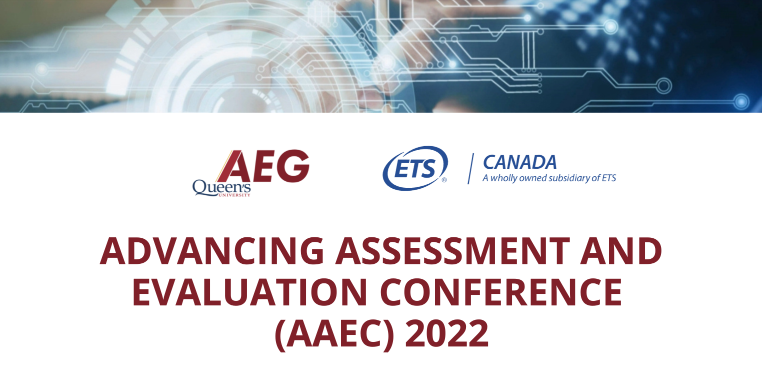
\includegraphics{Content/H.png}

Queen's University Assessment and Evaluation Group (AEG) and Educational Testing Services (ETS) Canada joined together to organize a virtual conference to promote partnerships and community across sectors (industry, academia, school districts) to spur innovation in assessment and education in Canada.

There were four themes of the conference:

\begin{enumerate}
\def\labelenumi{\arabic{enumi}.}
\tightlist
\item
  Advancing Assessment and Evaluation to facilitate learning in critical contexts
\item
  Advancing Assessment and Evaluation by leveraging technology
\item
  Advancing Assessment and Evaluation to promote equity and fairness
\item
  Advancing Assessment and Evaluation to promote language learning
\end{enumerate}

In addition to a poster session and networking opportunities, the conference consisted of four panel discussions, each facilitated by a discussant, on the four themes outlined above. The image below depicts the agenda for AAEC 2022.

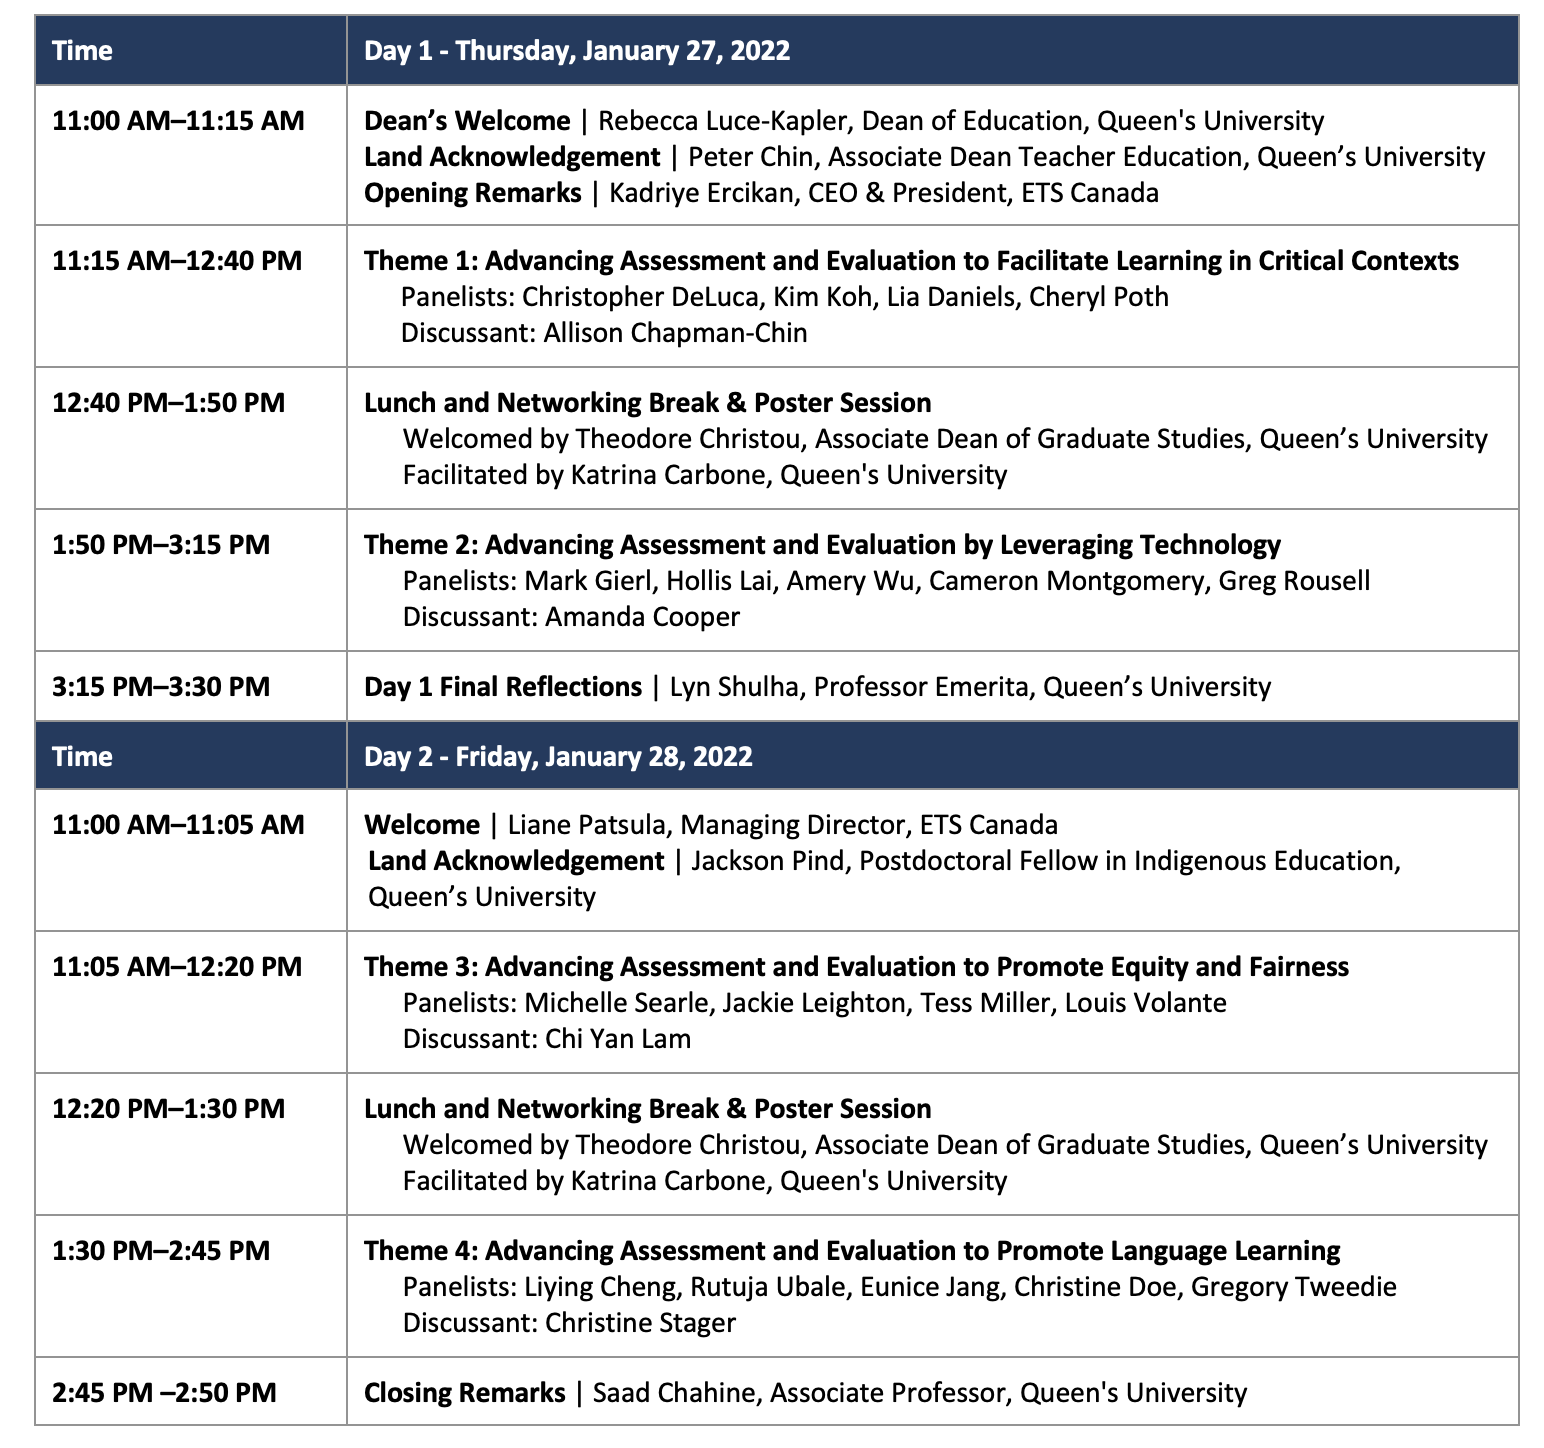
\includegraphics{Content/N.png}
\newpage

\hypertarget{speaker-information}{%
\chapter*{Speaker Information}\label{speaker-information}}
\addcontentsline{toc}{chapter}{Speaker Information}

\hypertarget{theme-1}{%
\section*{Theme 1}\label{theme-1}}
\addcontentsline{toc}{section}{Theme 1}

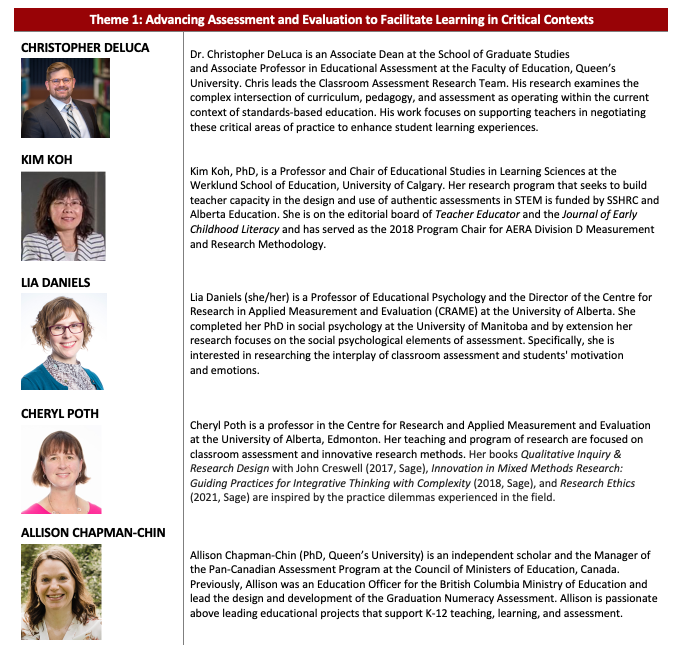
\includegraphics{Content/S1.png}

\newpage

\hypertarget{theme-2}{%
\section*{Theme 2}\label{theme-2}}
\addcontentsline{toc}{section}{Theme 2}

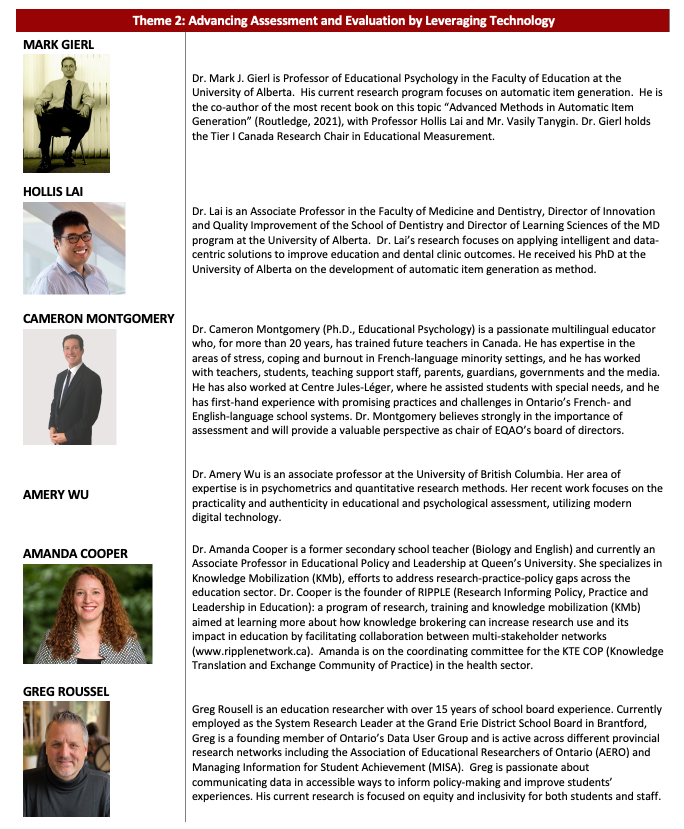
\includegraphics{Content/T2.png}

\newpage

\hypertarget{theme-3}{%
\section*{Theme 3}\label{theme-3}}
\addcontentsline{toc}{section}{Theme 3}

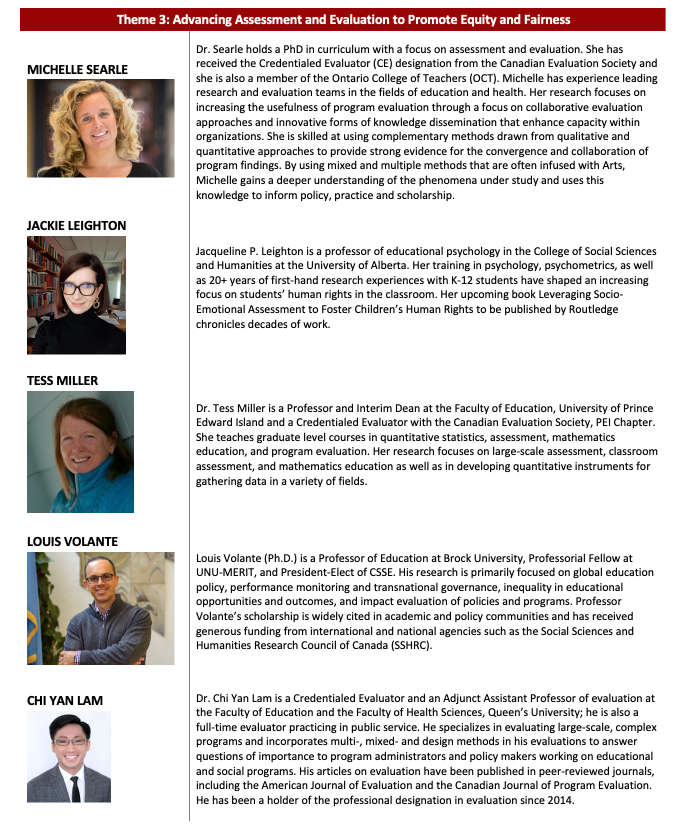
\includegraphics{Content/S3.png}

\newpage

\hypertarget{theme-4}{%
\section*{Theme 4}\label{theme-4}}
\addcontentsline{toc}{section}{Theme 4}

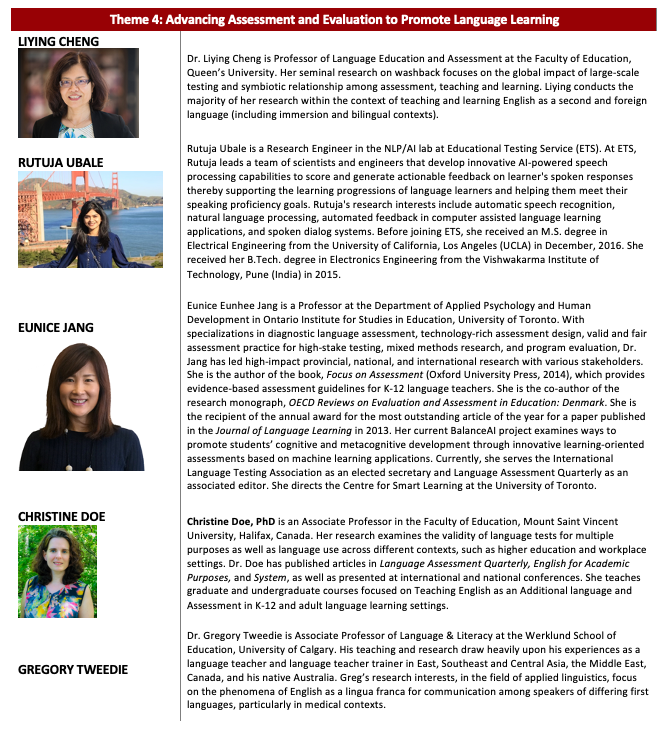
\includegraphics{Content/S4.png}

\newpage

\hypertarget{opening-remarks}{%
\chapter*{Opening Remarks}\label{opening-remarks}}
\addcontentsline{toc}{chapter}{Opening Remarks}

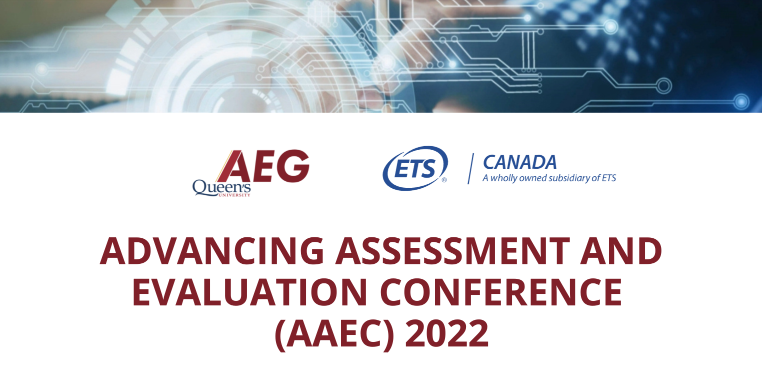
\includegraphics{Content/H.png}

\textbf{Kadriye Ercikan}, ETS Canada President, CEO

I am delighted to welcome you to the first Advancing Assessment and Evaluation Conference, organized jointly by ETS Canada and Queens University. Many thanks go to Liane Patsula, Managing Director of ETS Canada, and Saad Chahine, Assistant Professor of Measurement and Assessment at Queens University. I know that they have been working very hard to organize the event for several months.

More than 400 registrants from around the world have signed up for the conference. I am delighted to see so many colleagues and friends join us today. I know that we have a small assessment and evaluation community in Canada, and I am delighted to see this level of interest in the conference. I think it speaks to our need to connect and exchange ideas on important topics around assessment and evaluation. I hope that we will get to meet each other in person at the next conference.

I also want to acknowledge the critical juncture at which this conference is being held.

It's a critically important time for us to revisit the role of assessment and evaluation to meet current and future societal needs globally. Over the past two years, the COVID pandemic has disrupted education around the world. Practices in schooling, teaching, learning, and assessment have changed dramatically. Disparities in opportunity have grown with regard to the educational opportunities for quality education available to students from different cultural and social backgrounds. These disparities, which existed before the pandemic but may have been ignored or dismissed, have become clearer than ever, increasing concerns about equity and social justice.

Combined with these social changes, the impact of climate change is rapidly threatening life on earth as we know it.

There is heightened responsibility and urgency for reimagining education to meet immediate, significant needs, as well as long term possibilities. We need to focus on addressing inequities, and we need to focus on promoting collaboration and cooperation globally to address the pandemic, climate change, and future global challenges and transform education to meet new realities of lives of students and societal needs.

Assessments and evaluations have a critical role to play in transforming education. I highlight three goals in order to serve effective changes.

Assessments need:

\begin{itemize}
\item
  to be driven by the need to address inequities in societies;
\item
  to be grounded in sociocultural contexts of learners; and
\item
  to use technology to meet these goals instead of exacerbating inequities and adding new biases.
\end{itemize}

With these goals in mind, we need research to rethink the way assessments are designed, what kinds of data contribute to measurement, and using technology to advance the science of measurement.

To facilitate their use in addressing inequities, assessments need to engage students from different backgrounds effectively; provide quality measurement of all students; be adaptive to different abilities, backgrounds and interests; and need to be designed to optimize performance and information about learners to guide decisions about improving learning.

Grounding assessments in sociocultural context of learners requires taking this context into account in all aspects of assessments, including construct definition, task design, measurement, and interpretation. Assessments should reflect student cultural backgrounds and identities, not just those of mainstream cultures but for all students. They should also optimize ``equivalence of evidence'' instead of equivalence and standardization of testing and prioritize making contextualized interpretation of assessment.
Technology can play an important role in meeting some of the goals of assessments. Effective use of artificial intelligence can help provide feedback and guide and tailor assessments to diverse learners. Digital assessments can facilitate assessment of engagement in learning, not just assessment of outcomes. Data captured in digital assessments, such as response process data, can enhance measurement models. Adaptivity and interactivity made possible in digital assessments can be used to improve measurement.

We are hoping that this conference will serve to start conversations and collaborations. We hope that they will help to leverage our joint expertise and resources in advancing assessment and evaluation to facilitate the transformation in our critical educational and societal context.

Many thanks for joining us. Let's get the conversations started!

Kadriye

\hypertarget{theme1}{%
\chapter{Critical Contexts}\label{theme1}}

\hypertarget{theme-overview}{%
\section{Theme Overview}\label{theme-overview}}

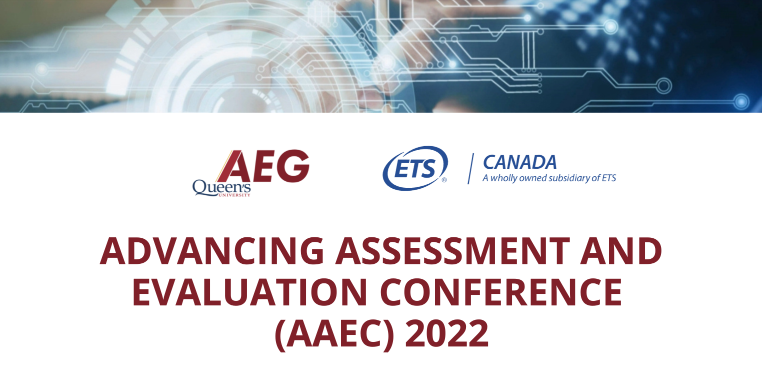
\includegraphics{Content/H.png}

\textbf{Description:} The COVID-19 pandemic caught education off guard. This panel was designed to begin the conversation about how we can advance assessment and evaluation to better understand learning in critical contexts and possibly offer strategies to facilitate learning and mitigate educational gaps to be better prepared for the next critical context.

The following questions were intended to inspire and generate ideas. The speakers did not need to address the questions directly.

\begin{itemize}
\item
  How has the pandemic affected learning and disparities in learning opportunities and outcomes?
\item
  How can assessment and evaluation help us measure and address disparities, opportunities and outcomes in learning that took place during the pandemic so that we can be better prepared for the next unexpected critical context?
\item
  How can assessment and evaluation address mental health struggles that will far outlast the pandemic and help all those affected move forward?
\end{itemize}

\newpage

\hypertarget{radical-change}{%
\section{Radical Change}\label{radical-change}}

\textbf{Author:} Christopher DeLuca, PhD

\textbf{Institution:} Queen's University

\textbf{Recommended Citation:}

\begin{quote}
DeLuca, C. (2022, January 27-28). \emph{Radical Change} {[}Paper presentation{]}. Advancing Assessment and Evaluation Virtual Conference: Queen's University Assessment and Evaluation Group (AEG) and Educational Testing Services (ETS), Kingston, Ontario, Canada.
\end{quote}

A year ago, I was asked to write an assessment provocation in relation to what, at that time, seemed like a nightmarishly long pandemic. Now, two years in, I continue to consider the effects of COVID on students, teachers, and society, now and inevitably for years to come. My previous provocation called for radical change, by drawing on the reflection that ``much educational assessment research {[}and indeed curriculum writ large{]} fell painfully short of addressing the pressing challenges before us; that much of our research reinforced the status quo, feeding past architectures of education and perpetuating systemic structures of reward, exclusion, and inequity'' (DeLuca, 2021, p.~167). Global calls for radical change permeate all sectors in response to COVID-19 but also in response to other mass crises -- the climate emergency, our racial reckoning, the necessity for Indigenous resurgence and remembering, and the mental health and opioid crisis which has only been exacerbated in COVID times, among others. However, these calls are particularly critical for education where radical truth has the power to transform teaching and learning into radical hope and a radical re-imagining for a better future (McGregor, Pind, \& Karn, 2020).

What have we learned from COVID -- two years in -- about curriculum and assessment? First, it is clear that curriculum and assessments predicated solely on discrete content knowledge are wholly inadequate in preparing us for the challenges we now face and will face in the future. While knowledge from across all the disciplines has been undeniably essential in responding to COVID, it has been the intersection of these knowledges that has mobilized our responses. Science alone is of little value without literacy to communicate and educate; mathematical modelling is illuminating but only when considered in relation to population psychology, politics, business, and economics. Historical analyses of previous pandemics are more beneficial when set within narratives, considered in relation to current population statistics and sciences, and reframed to today's social norms and desires. Perhaps more important, have been other skills and capacities beyond disciplinary knowledges, in combatting this crisis. What COVID and other global challenges have taught us is the importance of human wellness relationships and need to ``teach our children how to care for themselves, each other, and our world'' (DeLuca, 2021, p.~168). The emphasis here is on a curriculum of care, drawing largely from Nodding's work. She argues, ``against an education system that puts too much emphasis on academic achievement defined in terms of test scores and the acquisition of information'' and instead believes students should ``be given opportunities to learn how to care for themselves, for other human beings, for the natural and human-made worlds, and for the world of ideas'' (Noddings, 2005, p.~2).

At the heart of this argument is a radical change away from priorities of testing siloed knowledges towards a curriculum that engage students in learning to care, which demands learning about subjects, the self, community, and skills. It is a curriculum of social action with calls for authentic and deeply integrated assessments. Importantly, this orientation draws on an integrated curricular model, one purported by the OECD (2018, p.~4), and which helps learners ``examine local, global and intercultural issues, understand and appreciate different perspectives and world views, interact successfully and respectfully with others, and take responsible action toward sustainability and collective well-being''. And it both aligns with and extends discourse surrounding 21st century learning competencies -- collaboration, creativity, supporting equity, communication, self-regulated learning, metacognition, digital literacy, and problem solving (Pellegrino, 2017) -- by placing learners in direct responsibility for personal and social change through their learning.

Calls for a more caring-centred curriculum are not new, and there is ample evidence that such a model of education is possible and works. Research from Suparna Roy -- an Assessment and Evaluation Group alumni -- has shown the possibility and value of an integrated, community service-oriented curriculum in her study of a sixth-grade class (Roy, 2019). Through her year-long project with students and teachers, she worked to implement curriculum that purposeful prioritised learning-to-serve through an inquiry pedagogy that integrated disciplinary learning with student collaboration and community engagement. Data from her study show that such a model cultivated selflessness in students, helped regulate students' emotions, encouraged prosocial behaviours, and built and deepened relationships in the classroom and within community. Similarly, in our recent work with teachers committed to integrated teaching models in Ontario elementary and secondary levels (Dubek, DeLuca, \& Rickey, 2021), specifically drawing on a STEAM approach, we found that they universally endorsed this approach and recognized it for teaching foundational 21st century learning skills while also addressing content knowledge expectations. Yet most importantly, these teachers noted that an integrated curricular orientation provoked learning grounded in critical social contexts, allowing them to apply their learning to real social and community concerns ---- an integrated curriculum of care.

A necessary imperative across this research (Dubek et al., 2021; Roy, 2019) was the need to reframe assessment to meaningfully support learning within an integrated model. This reframing has involved four key features. Firstly, traditional summative assessments focussed primarily on siloed content learning no longer occurred at the end of learning cycles, but rather were repositioned as smaller check points throughout students' learning journeys to ensure they had the requisite knowledge to effect change in relation to their critical context, because knowledge is the precursor to action. Second, summative assessments were still deemed essential but redesigned as fully integrated and authentic opportunities to culminate learning in actions and applications, often through collaborative experiences that assessed and prioritised a range of student learning skills and capacities. Third, formative assessment, including assessment for and as learning, became a dominant driver for learning a both individual and group levels. Specifically, multiple feedback mechanisms (i.e., self-documentation, goal setting, reflection, self-testing, protype testing, making metacognitive processes explicit, interactional self-assessment, peer assessment, and dialogue) were infused throughout the learning process to stimulate learning. Lastly, assessment was not limited to the classroom; community members and parents were brought into assessment dialogues in active ways to support student learning but also as a means to cultivate deeper relationships.

In closing, I return to the challenge before us: the painful shortfall of much educational assessment research and practice to support, promote, and report on a curriculum of care. For radical change in education, we must be willing to critically dismantle the assessments of the past, and establish assessment processes that attend to the collaborative, relational, and complex learning that is at the heart of learning to care. Dominant priorities of accountability and broad conceptions of assessment manifest through comparisons, standardization, and testing need to be reconsidered and replaced with authentic, person-centred, and locally valid assessments. Accountability should be measured in the actions of our students not in their test scores. 

\textbf{References}

DeLuca, C. (2021). Towards more radical assessment systems. In Wyatt-Smith, Adie, Nuttall (Eds.), Teacher Performance Assessments as a Cultural Disruptor in Initial Teacher Education: Standards, Evidence and Collaboration (pp.~167-170). Singapore: Springer.

Dubek, M. DeLuca, C., \& Rickey, N. (2021). Unlocking the potential of STEAM education: How exemplary teachers navigate assessment challenges. The Journal of Educational Research, 114(6), 513-525.

McGregor, H. E., Pind, J., \& Karn, S. (2020). A ``Wicked problem'': Rethinking history education in the Anthropocene. Faculty of Education, Queen's University.

Noddings, N. (2005). The challenge to care in schools: An alternative approach to education (2nd ed), New York, NY: Teachers College Press.

OECD. (2018). Preparing our youth for an inclusive and sustainable world: The OECD PISA global competence framework. \url{https://www.oecd.org/pisa/Handbook-PISA-2018-Global-Competence.pdf}

Pellegrino, J. W. (2017). Teaching, learning and assessing 21st century skills. In S. Guerriero (Ed.), Pedagogical knowledge and the changing nature of the teaching profession, Educational Research and Innovation (pp.~223--251). OECD Publishing.

Roy, S. (2019). A pedagogy of selflessness: A multiple case study exploring the cultivation and expression of student selflessness in an Ontario Grade 6 classroom. Unpublished doctoral dissertation. Kingston, ON: Queen's University.

\newpage

\hypertarget{reimaging-educational-assessment-in-the-new-normal}{%
\section{Reimaging Educational Assessment in the New Normal}\label{reimaging-educational-assessment-in-the-new-normal}}

\textbf{Author:} Kim Koh, PhD

\textbf{Institution:} Werklund School of Education, University of Calgary

\textbf{Recommended Citation:}

\begin{quote}
Koh, K. (2022, January 27-28). \emph{Reimaging Educational Assessment in the New Normal} {[}Paper presentation{]}. Advancing Assessment and Evaluation Virtual Conference: Queen's University Assessment and Evaluation Group (AEG) and Educational Testing Services (ETS), Kingston, Ontario, Canada.
\end{quote}

\textbf{Introduction}

The unprecedented COVID-19 pandemic is a global crisis, which has led to many disruptions to education. In addition to the coronavirus, the world has increasingly faced various threats due to racial injustice and violence, different ideologies in politics and vaccine, economic recession, cyber-terrorism, and climate change. Digital divide is one of the many social inequalities. At the beginning of the pandemic, more than 1.2 billion students in the world were forced to learn remotely using technology, while their teachers had to adapt to teaching and assessing remotely (UNESCO, 2020). However, not every student has access to the latest digital tools and the fastest Internet connectivity. This unplanned and rapid move to digital learning environments has widened inequalities between students from low- and high-socioeconomic status backgrounds. For instance, according to OECD's Program for International Student Assessment data (Schleicher, 2020), 95 per cent of students in economically, developed countries (e.g., Switzerland, Norway, Austria) have a computer to use for their schoolwork, whereas only 34 per cent of students in developing countries (e.g., Indonesia) have access to a computer at home. Such a digital divide has perpetuated or even exacerbated existing disparities in educational opportunities and outcomes.

A lack of technological resources and support can disrupt students' online instruction and assessment. This constitutes an issue of equity and social justice. Even after the distribution of free computers and tablets to many students later on in the pandemic, there is growing evidence that online teaching, learning, and assessment can pose challenges to students and their teachers. For example, teachers often lack time to design and modify instructional activities and assessment tasks for online instruction or must constantly shift their teaching and assessment modality from in-person to online, potentially causing disruptions to students' learning. Many students lack motivation to attend online classes or may even become disengaged from learning and completing assignments. Some even decide to drop out of school during the pandemic. Even when supplied with a free technology device, students from disadvantaged family backgrounds or from marginalized communities may feel that they are not sufficiently equipped to use the technology effectively. If their academic performance is assessed through a digital assessment, the data may be distorted, thereby resulting in an inaccurate evaluation of what they know and can do (National Academy of Education, 2021).

Two years into the pandemic, many students are now at risk for suffering from learning loss. Some students and parents have also faced worsening mental health due to prolonged lockdown measures and greater financial burdens (Oster et al., 2021). Although schools have reopened for students, strict physical distancing, restrictions with sharing learning materials and equipment, and minimal social interactions have made group work and other activities very difficult in and out of the classroom. For example, in STEM (science, technology, engineering, and mathematics) learning, many informal learning opportunities such as visiting museums, summer camps, field trips, and after-class activities, are no longer possible. In the report Raising Canada 2020 (Children First Canada, O'Brien Institute for Public Health, \& Alberta Children's Hospital Research Institute, 2021), Canadian students were found to be in danger of increasing levels of anxiety and depression due to the negative consequences of the COVID-19 pandemic. These consequences include poverty and food insecurity, child abuse and neglect, social isolation, and physical inactivity. Research has shown that students' mental health problems could compromise the quality of their learning, ultimately leading to lower academic performance.

At this juncture, the many waves of new variants, including the highly transmissible Omicron variant, have led to school closures, and many students have had to resort to emergency remote learning again. Alibudbud (2021) has pointed out that prolonged online learning can result in negative mental health consequences, including increased anxiety and absenteeism among students. In an online learning environment, some students may be neither tech savvy nor willing to speak and turn on their video cameras. This may make it more difficult for teachers to assess student engagement and motivation to learn, as well as other learning outcomes. However, some studies (e.g., Cavanaugh \& Jacquemin, 2015) in higher education have found no significance difference in student learning outcomes when comparing the online and face-to-face modalities. Taken together, these suggest that disparities in learning opportunities and outcomes in K‒12 schools and postsecondary institutions in the current critical context may widen compared to their condition before the pandemic. Future research needs to focus on understanding disparities in educational opportunities and outcomes (i.e., cognitive, affective, and physical) in online and blended learning environments.

\textbf{Alternative Assessments to Address Disparities, Opportunities, and Outcomes in Learning}

It is time for educational researchers and educators to reflect on, redefine, and identify these constructs in the new normal. For example, what are the new learning disparities in a digital age? Are there equitable educational opportunities for those who are marginalized (e.g., newcomers, English language learners, low-income families, racialized communities, children with special needs)? What are the essential educational and psychological outcomes (i.e., literacy and numeracy, competencies or soft skills, social and emotional well-being) that matter to students, teachers, and parents within the current critical context and beyond?

The functionalities of some of the new assessment methods (e.g., big data, learning analytics, and serious games) are worth investigating. Even before the pandemic, effective use of big data could help inform policymakers' decisions on reallocating resources to aid schools and marginalized communities (e.g., new immigrants, refugees, Indigenous Canadians). Likewise, learning analytics enable teachers to make instructional and assessment decisions based on real-time data. Through such data, a teacher can assess, monitor, and respond instantly to a student's understanding of the learning material as well as a student's social emotional skills and other competencies. Such a formative assessment or assessment for learning strategy not only helps a teacher to provide timely, quality feedback to improve student learning and performance, but also enables the teacher to adjust teaching or to differentiate instruction. Using such strategies allows teachers to create more equitable learning opportunities to meet the need of every student. Research in higher education has advocated for the leveraging of big data and learning analytics in the assessment of student learning in an online environment. For instance, according to Martin and Ndoye (2016), learning analytics enables instructors to download, analyze, and interpret student data immediately so that students who are at risk for learning and social or emotional problems can be identified as early as possible in a course and intervention strategies can be developed to remedy such problems.

Many educators may wonder what essential students' learning outcomes need to be assessed and monitored within the current critical context. The existing formal and informal assessment methods can be reviewed to determine whether they still provide reliable and valid data that help inform teachers' instructional practices and students' learning in online, face-to-face, and blended learning environments. A heavy focus on administering large-scale assessments during the pandemic and using the resulting data to make important decisions about students and schools (e.g., placement, admission, ranking of schools, allocation of resources to schools) may result in bias and injustice due to the lack of equitable learning opportunities, resources, and social emotional support for students. Due to the unpredictability of the pandemic, high-stakes examinations have often been cancelled at the last minute. Even if students are able to sit for these exams, their stress and anxiety levels may increase given the new social and physical restrictions, face masking, and plexiglass barriers. Instead of mid-year and end-of-year summative assessments, formative assessments (e.g., clearly defined success criteria and performance standards in a rubric, timely and high-quality feedback, and self-assessment) could be incorporated into teachers' instructional plans to help students to become more engaged in the learning process and more responsible for monitoring their own progress toward the learning goals that they themselves and their teachers have established. Further, classroom assessment may focus more on monitoring individual students' learning progression and making learning visible for students (Hattie, 2012). This will support students' development of a growth mindset (Dweck, 2006). There is an urgent need to focus on the design and development of curriculum sensitive and culturally responsive assessment tools and strategies, which measure students' growth in learning over time and which serve diagnostic purposes.

During this critical time, authentic and formative assessments need to be promoted in day-to-day teaching and learning contexts so that students are given more opportunities to develop and demonstrate a variety of competencies (e.g., critical thinking, complex problem-solving, creativity and innovation, self-regulated learning, self-efficacy, grit and resilience, perseverance, risk-taking, and entrepreneur mindset). These competencies can help prepare them for life and studies after the pandemic, as well as their future careers. Authentic assessment replicates real-world problems and performance standards typically faced by professionals in the field (Koh, 2017; Wiggins, 1989). Students can be encouraged to complete their tasks under the guidance and mentorship of their teachers or of educational assistants who can provide timely and quality feedback using well-developed rubrics. Authentic assessment also creates opportunities for students to produce innovative and creative products or performances, thereby preventing them from cheating and committing plagiarism. Other forms of formative assessment, such as self-assessment, can be seamlessly incorporated into authentic assessments so that students can be encouraged to monitor their own progress and take more responsibility for their own learning. In the long run, this can help develop their self-directed learning skills, confidence, and academic self-efficacy.

\textbf{Enhancing Teachers' Assessment Capacity in the New Normal}

In a world plagued by the uncertainty of new variants, intense racial tensions, and other social injustice issues, K-12 teachers' capacity to design, modify, select, and use assessment methods or tasks that are culturally responsive to the learning needs of individual students has become increasingly important. It may be necessary to create more opportunities for teachers, researchers, assessment specialist, instructional designers, and IT professionals to dialogue and collaborate in the design of effective classroom assessments and learning environments. Additionally, it is important to consider how advances in technology (e.g., virtual reality, augmented reality, machine learning, and artificial intelligence) can be leveraged to design alternative forms of assessments, such as authentic assessments and online formative assessments (e.g., automated feedback system), especially if teaching and learning have to constantly shift from in-person to online or must take place in a blended environment. Furthermore, how to accommodate assessment modes for students with special needs must also be taken into account.

In addition to the design of assessment and leveraging technology, teacher capacity building is equally important. Hence, teachers need to be supported through the provision of high-quality professional learning and development opportunities. Teachers' competencies in providing feedback and in both designing and using rubrics and exemplars are essential for effective assessment for learning or formative assessment practice, to be carried out in face-to-face, online, and blended learning environments (Koh et al., 2021). The provision of timely and descriptive feedback can also reduce students' level of stress and anxiety about their academic performance. It is also necessary to focus more on assessing students' growth in each subject area. Thus, report cards could adopt a narrative format, highlighting students' strengths and areas for improvement and orienting them toward a growth mindset (Dweck, 2006). Similar to the teachers in Australia, Scotland, and Finland, teachers in other parts of the world including Canada, need to be given more agency and autonomy in the assessment and evaluation of students' work. School leaders and parents should put their trust in teachers' professional judgement. Online moderation panels may be set up for teachers to moderate students' work. Moderation conversations serve as a powerful mechanism for teachers' professional learning and growth in assessment literacy (Klenowski \& Wyatt-Smith, 2014). Such a mechanism is now more important than ever so that teachers will not feel that they are fighting the pandemic in silos.

Finally, teachers need to be aware of digital divide, which may impact the technology that their students have and their ability to access and engage with learning materials, readings, and assessment tasks. Some students may not be able to complete assignments on time. Online learning environments need to be safe, caring, and supportive for every student. The use of technology in teaching, learning, and assessment has increasingly become the norm during the COVID-19 pandemic. Therefore, it is important for teachers to know how to create online environments that are accessible and flexible, and that provide students with options for participation, taking into account the challenges and constraints students may encounter (Correia, 2020). Online forum or discussions should be evaluated based on the quality of discussion (i.e., thoughtful questions and answers or reflections), not on the number of posts and replies. More intentional scaffolding of online learning activities and assessment tasks is necessary. Providing students with effective rubrics and educative exemplars can give them a sense of agency in assessing and monitoring their own learning in face-to-face, online, and blended learning environments (Koh et al., 2021).

Designing Assessment for Learning: Care, Hope, Collaboration, and Growth
Instead of obsessing with summative assessments for accountability and grading, frequent formative assessments can be seamlessly integrated into the learning process in a face-to-face, online, or blended learning environment. Teaching is about engaging both a student's mind and heart. Therefore, there is a need for teachers to use assessment to support student learning (i.e., Assessment for and as Learning). This will enable students to develop soft skills including growth mindsets and other 21st-century competencies, which are deemed necessary for their future success in both personal and professional lives. Despite technological inequalities in some parts of the world, online education and blended education are likely to become the norm in a post-pandemic era. Thus, it is important for teachers to consider collaborating with assessment specialists, instructional designers, and IT professionals to design effective online assessment tools (e.g., authentic assessments, projects, serious games) and create learning environments that focus on care, hope, collaboration, and growth. For instance, an integration of virtual reality into authentic assessments can help simulate experiences, similar to those in the real world so that students can still visit a museum or take a tour virtually despite pandemic restrictions (Koh et al., 2022). Such efforts can then help alleviate mental health struggles among students, especially for those who come from historically underserved backgrounds (i.e., first-generation students, low-income students, ethnic and racial minority students, and newcomers and refugees).

\textbf{Conclusion}

In this paper, I provide some thoughts and recommendations to help address disparities, opportunities, and outcomes in learning due to the pandemic crisis. I sincerely believe that educational researchers, PreK‒16 educators and administrators, policymakers, students, parents/guardians, non-profit organizations, and the public within each province or district must come together to engage in a meaningful, genuine dialogue as well as to co-create solutions and take immediate actions to reduce educational disparities in the current critical context. Such a collaborative effort is necessary on a continuing basis so that Canadian schools and higher education institutions can be better prepared for the next global crisis.

\textbf{References}

Alibudbud, R. (2021). On online learning and mental health during the COVID-19 pandemic: Perspectives from the Philippines. Asian Journal of Psychiatry, 66, \url{https://dx.doi.org/10}. 1016\%2Fj. ajp.2021.102867

Cavanaugh, J. K., \& Jacquemin, S. J. (2015). A large sample of comparison of grade based student learning outcomes in online vs.~face-to-face courses. Online Learning, 19(2).

Children First Canada, O'Brien Institute for Public Health, \& Alberta
Children's Hospital Research Institute. (2021). Top 10 threats to childhood in Canada and the impact of COVID-19. Raising Canada 2020 Report. \url{https://childrenfirstcanada.org/wp-content/uploads/2021/} 09/Raising-Canada-Report\_2020\_Updated.pdf

Correia, A. (2020). Healing the digital divide: During the COVID-19 pandemic. The Quarterly Review of Distance Education, 21(1), 13‒21.

Dweck, C. S. (2006). Mindset: The new psychology of success. Ballantine Books.

Hattie, J. (2012). Visible learning for teachers: Maximizing impact on learning. Routledge.

Klenowski, V., \& Wyatt-Smith, C. (2014). Assessment for education: Standards, judgement and moderation. Sage Publications, Ltd.

Koh, K. (2017). Authentic assessment. In G. W. Noblit (Ed.), Oxford Research Encyclopedia of Education. Oxford University Press.

Koh, K., Chapman, O., \& Lam, L. (2022). An integration of virtual reality into the design of authentic assessments for STEM learning. In S. Keengwe (Ed.), Handbook of research on transformative and innovative pedagogies in education. IGI Global.

Koh, K., Kowch, E., Grant, K., Bene, R., \& Liu, S.M. (2021). Understanding undergraduate students' and instructors' perceptions of and experiences with exemplars. Report. Taylor Institute for Teaching and Learning, University of Calgary.

Martin, F., \& Ndoye, A. (2016). Using learning analytics to assess student learning in online courses. Journal of University Teaching \& Learning Practice, 13(3), Article 7.

National Academy of Education. (2021). Educational assessments in the COVID-19 era and beyond. \url{https://naeducation.org/wp-content/uploads/2021/02/Educational-Assessments-in-the-COVID-19-Era-and-Beyond.pdf}

Oster, E., Jack, R., Halloran, C., Schoof, J., McLeod, D., Yang, H., Roche, J., \& Roche, D. (2021). Disparities in learning mode access among K‒12 students during the COVID-19 pandemic, by race/ethnicity, geography, and grade level --- United States, September 2020‒April 2021. Morbidity and Mortality Weekly Report, 70(26), 953‒958.

Schleicher, A. (2020). Education disrupted -- education rebuilt: Some insights from PISA on the availability and use of digital tools for learning. OECD education and skills today. \url{https://oecdedutoday.com/coronavirus-education-digital-tools-for-learning/}

UNESCO. (2020). Education: From disruption to recovery. \url{https://en.unesco.org/covid19/} educationresponse

Wiggins, G. (1989). A true test: Toward more authentic and equitable assessment. Phi Delta Kappan, 70(9), 703‒713.

\newpage
\pagestyle{fancy}

\hypertarget{a-critical-turning-point-wellness-as-a-framework-for-classroom-assessment}{%
\section{A Critical Turning Point: Wellness as a Framework for Classroom Assessment}\label{a-critical-turning-point-wellness-as-a-framework-for-classroom-assessment}}

\fancyhead[LE,RO]{\nouppercase{\truncate{0.5\headwidth}{\rightmark}}}
\fancyhead[LO,RE]{\nouppercase{\truncate{0.5\headwidth}{\leftmark}}}

\textbf{Author:} Lia Daniels, PhD

\textbf{Institution:} Centre for Research in Applied Measurement and Evaluation College of Social Sciences, University of Alberta

\textbf{Recommended Citation:}

\begin{quote}
Daniels, L. (2022, January 27-28). \emph{A Critical Turning Point: Wellness as a Framework for Classroom Assessment} {[}Paper presentation{]}. Advancing Assessment and Evaluation Virtual Conference: Queen's University Assessment and Evaluation Group (AEG) and Educational Testing Services (ETS), Kingston, Ontario, Canada.
\end{quote}

Please note some content of this paper is taken directly from Daniels et al.~2021.

It seems almost common wisdom that students should be motivated to perform well on assessments and that good performance on assessments should, in turn, increase future motivation (Wise \& Smith, 2016). This intuitive positive association, however, often does not line up with the reality of many students. More than ever, students report debilitating test anxiety about low performance or and appear disinterested in course content even when they get high test scores (Wise \& Smith, 2016). As a motivation researcher, I look at this situation and see an oversight that can be corrected by integrating contemporary perspectives on assessment and motivation. Importantly, by considering motivation and its associations with wellness as a framework for classroom assessment, the field may be able to improve students' wellness while meeting the standards of fair assessment. The challenges that COVID-19 has introduced in terms of both undermining student wellbeing and challenging assessment practices may afford a critical turning point that the field would be wise to seize.

\textbf{Motivation and Wellness}

This year the European Lifelong Learning Platform dedicated their annual position paper to the following question: ``How can we rethink assessments to contribute to well-being rather than hamper it?'' As an invited member of their Expert Task Force (2021), I recommended that they consider using motivation theory to allow combined thinking on wellness and assessment. I based this recommendation on decades of evidence showing consistent small to medium negative associations between intrinsic motivation and indicators of poor wellness like anxiety and stress and similar positive associations with indicators of wellness such as engagement, self-efficacy, and satisfaction (Howard et al., 2020). In light of COVID-19, it is critically important to enhance assessment not just in terms of delivery modes, online security, and scoring, but in terms of students' overall wellness - and motivation theory is an excellent framework for this purpose.

\textbf{Hasn't Assessment Literature been impacted by Theories of Motivation?}

In a recent chapter (Daniels et al., 2021), my co-authors and I reviewed 11 current textbooks on classroom assessment by a range of authors and publishers. We found that just over 60\% of textbooks included the term ``motivation'' in the index. When we looked deeper into the indexed term, it seemed common for authors to discuss how motivation can influence a student's overall experience of academic success as measured by graded assessments. A few motivation constructs like intrinsic and extrinsic motivation, goals, self-regulation, and efficacy were introduced as were ways motivation was negatively impacted by summative assessments.

The following suggestions were offered across the textbooks:
• provide students with the autonomy to construct their own summative assessments
• use portfolios to allow students to choose the content that will count towards their final grade
• create questions related to the student's interests and strengths
• provide students with written feedback along with their grade as soon as possible so that they know what to focus on for following assessments

Additionally, the authors commonly suggested that the best way to enhance intrinsic motivation was to move away from summative and towards formative assessment practices (Fetsco \& McClure, 2005; Gardner, 2012). Affirming this recommendation, many of the assessment textbooks that focus exclusively on formative assessment dedicate substantial room to also describing the relationship with motivation (e.g., Chappuis, 2015; Marzano, 2011). As either a common recommendation or separate textbook, the focus on formative assessment as the best means to support motivation fails to tackle the motivational potential or peril of summative assessment. This is particularly negligent because summative assessment remains omnipresent. For example, in a recent sample of undergraduate preservice teachers we surveyed (n = 226), only 37\% said that their recent course used formative assessment whereas 96\% said their course involved graded summative assessments (unpublished).

\textbf{Motivation Theory as a Framework for Assessment}

As guilty as the assessment literature is about ignoring motivation theory, so too the field of achievement motivation is guilty of neglecting assessment practices. Although principles and recommendations abound for how motivation theory can support instructional practice (Linnenbrink-Garcia et al., 2016), rarely are such recommendations extended explicitly to assessment practices. Consider the following statement which is taken from a paper exemplifying how to create motivating classrooms:

\begin{quote}
Your paper is due on Monday. As a way of helping you write a well-researched paper,we are going to\ldots the school library. The reason we are going to the library is to find the information you need\ldots. While there, you may be tempted to goof off, but students \ldots{} have found that a trip to the library was a crucial part of writing an excellent paper\ldots. Reeve 2009, p.~169
\end{quote}

Amongst the motivation strategies related to the process, the assessment, namely a paper, is not contextualized by motivation theory at all. It is the only option - stated directly and plainly. This is an example of how researchers encourage teachers to support motivation through their instruction, but do not intentionally apply the principles to assessment. This concern was foreshadowed 30 years ago by motivation researcher Carol Ames:

\begin{quote}
We may find teachers who are very effective in designing tasks that offer variety and appropriate challenges to students. These same teachers, however, may use evaluation practices that encourage social comparison\ldots. {[}T{]}hese structures need to work in concert, they need to be coordinated\ldots. {[}and if not{]} motivation outcomes are confused. (Ames, 1992 p.~266)
\end{quote}

We chose self-determination theory (SDT; Ryan \& Deci, 2017) as one motivation theory that could be used as a framework for classroom assessment. According to SDT we can distinguish different types of motivation by focusing on forms of motivation that come from internal compared to external sources. On one end of the continuum, extrinsic motivation is listed as the most external form of motivation. Extrinsic motivation is typically experienced when individuals feel pressured by someone or something to act, feel, behave, or think in specific ways or to avoid certain outcomes (Ryan \& Deci, 2017). When teachers use summative assessments to compel students to learn specific content, behave a certain way, or receive a particular reward (even a gold star), they tap into students' extrinsic motivation. And extrinsic motivation is often associated with good grades, suggesting that indeed summative assessment can leverage extrinsic motivation to compel students to achieve (Ratelle et al., 2007). However, researchers have also shown that extrinsic motivation is associated with reduced valuing of certain activities (Deci \& Ryan, 2008), lower interest and enjoyment in the task, less persistence, more anxiety, procrastination, and dishonesty (Vansteenkiste et al., 2008).
There are three other forms of motivation that become increasingly internal to the person (Ryan \& Deci, 2017), enroute to intrinsic motivation on the other side of the continuum. Intrinsic motivation is the most internal form of motivation and argued to be the most beneficial for students. Intrinsic motivation is defined as ``{[}the{]} natural inclination toward assimilation, mastery, spontaneous interest and exploration that is so essential to cognitive and social development and that represents a principal source of enjoyment and vitality throughout life'' (Ryan \& Deci, 2000, p.~70). Intrinsic motivation originates purely from within the self, as one experiences and enacts volition and choice (Vansteenkiste et al., 2006) - it is freedom from external pressure and control. When students are intrinsically motivated they tend to experience more positive emotions and less anxiety, be more creative and deeper learners, persist in the face of challenge, and experience more interest, enjoyment, and satisfaction in learning (Ryan \& Deci, 2017). These are the kinds of learners I want and I do not want to fall victim to Ames' admonition to undo good instructional practices with contradictory assessment that can undermine student wellness.

In short, when teachers and parents expect students to be motivated by assessment, they view assessment as an external motivator. However, because summative assessment is external to the student, it may appear incompatible with intrinsic motivation. I suggest that this is not true and that instead we can support intrinsic motivation and its associations with student wellness even during assessment by meeting students' basic psychological needs of autonomy, competence, and relatedness. Autonomy is defined as experiencing behaviours as freely chosen, with oneself at the origin of the behaviour (Niemiec \& Ryan, 2009). The need for competence is defined as ``the experience of behaviour as effectively enacted'' (Niemiec \& Ryan, 2009, p.~135). In other words, in order for individuals to feel competent, an activity should be neither too difficult nor too easy, and allow them to feel effective in their environments. The psychological need for relatedness is defined as feeling close and connected to others, through supportive and satisfying close relationships.

When the basic psychological needs are met, otherwise external forms of motivation - even assessment - can become more internal and by extension lead to the pleasant outcomes associated with intrinsic motivation. The main advantage of framing assessment through SDT is the ability to anchor all assessment conversations and decisions to the theoretical and empirical richness of motivation theory. In other words, whether dealing with formative or summative assessments, multiple choice tests or authentic performances, and any number of feedback models, SDT can provide the conceptual framework (Bordage, 2009) to centre the wellness of students to the design of classroom assessment including the target of assessment, its measurement and format, as well as the interpretation and communication without compromising its reliability or validity. I offer the following Summary Table and direct readers to the full chapter for more details.

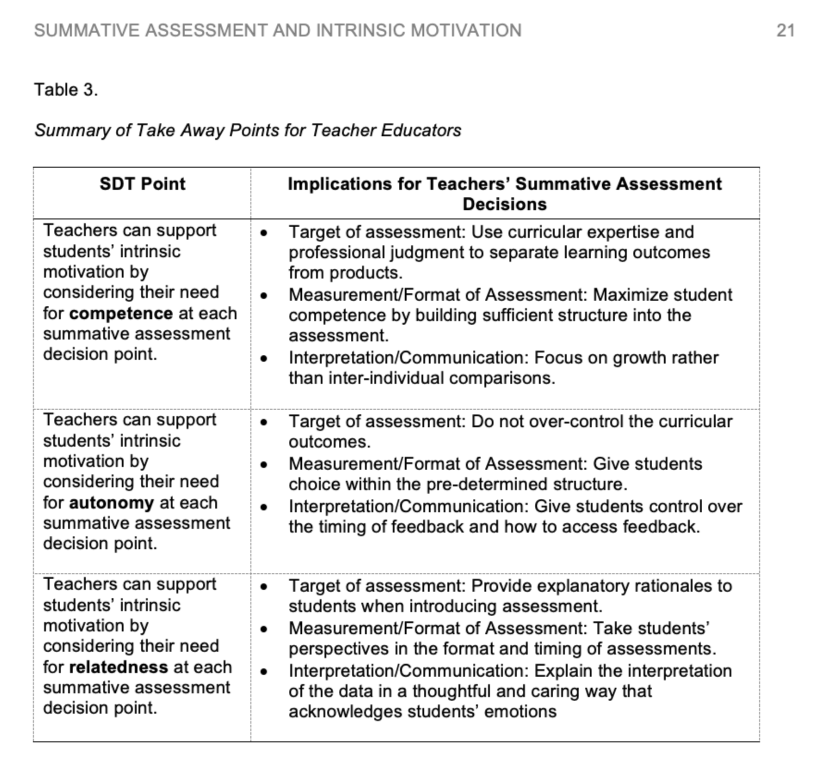
\includegraphics{Content/Table3.png}

\textbf{References}

Ames, C. (1992). Classrooms: Goals, structures, and student motivation. Journal of Educational Psychology, 84(3), 261--271.

Bordage, G. (2009). Conceptual frameworks to illuminate and magnify. Medical education, 43(4), 312-319.

Chappuis, J. (2015). Seven strategies of assessment for learning (2nd ed.). Pearson Assessment Training Institute.

Daniels, L. M., Pelletier, G., Radil, A. I., \& Goegan, L. D. (2021). Motivating assessment: How to leverage summative assessments for the good of intrinsic motivation. In Sharon Nichols \& Divya Varier (Eds.), Theory to practice: Educational psychology for teachers and teaching (Teaching on Assessment).

Deci, E. L., \& Ryan, R. M. (2008). Self-determination theory: A macrotheory of human motivation, development, and health. Canadian Psychology, 49, 182--185.

Fetsco, T., \& McClure, J. (2005). Educational Psychology: An integrated approach to classroom decisions. Allyn and Bacon.
Gardner, J. (Ed.) (2012). Assessment and learning. SAGE Publications Ltd.

Howard, J. L., Chong, J. X., \& Bureau, J. S. (2020). The tripartite model of intrinsic motivation in education: A 30‐year retrospective and meta‐analysis. Journal of Personality, 88(6), 1268-1285.

Linnenbrink-Garcia, L., Patall, E. A., \& Pekrun, R. (2016). Adaptive motivation and emotion in education: Research and principles for instructional design. Policy Insights from the Behavioral and Brain Sciences, 3(2), 228-236.

Marzano, R. J. (2011). Formative assessment \& standards-based grading. Solution Tree Press.

Niemiec, C. P., \& Ryan, R. M. (2009). Autonomy, competence, and relatedness in the classroom: Applying self-determination theory to educational practice. School Field, 7(2), 133-144.

Ratelle, C. F., Guay, F., Vallerand, R. J., Larose, S., \& Senécal, C. (2007). Autonomous, controlled, and amotivated types of academic motivation: A person-oriented analysis. Journal of Educational Psychology, 99(4), 734-746.

Reeve, J. (2009). Why teachers adopt a controlling motivating style toward students and how they can become more autonomy supportive. Educational Psychologist, 44(3), 159-175. Ryan, R. M., \& Deci, E. L. (2017). Self-determination theory: Basic psychological needs in motivation development and wellness. Guilford Publishing.

Vansteenkiste, M., Lens, W., \& Deci, E.L. (2006). Intrinsic versus extrinsic goal contents in self-determination theory: Another look at the quality of academic motivation. Educational Psychologist, 41, 19-31.

Vansteenkiste, M., Ryan, R. M., \& Deci, E. L. (2008). Self-determination theory and the explanatory role of psychological needs in human well-being. In L. Bruni, F. Comim, \& M. Pugno (Eds.), Capabilities and happiness (pp.~187--223). Oxford University Press.

Wise, S.L., \& Smith, L.F. (2016). The validity of assessment when students don't give good effort In Brown, G.T.L, \& Harris, L.R. (Ed), Handbook of human and social conditions in assessment (pp.~204-220). Routledge.

\newpage
\pagestyle{fancy}

\hypertarget{educational-assessment-dilemmas-and-opportunities-from-the-covid-19-pandemic-evolving-perspectives-from-a-zoom-box-instructor-to-blurry-eyed-parent}{%
\section{Educational Assessment Dilemmas and Opportunities from the Covid 19 Pandemic: Evolving Perspectives from a Zoom `box' Instructor to Blurry-eyed Parent}\label{educational-assessment-dilemmas-and-opportunities-from-the-covid-19-pandemic-evolving-perspectives-from-a-zoom-box-instructor-to-blurry-eyed-parent}}

\fancyhead[LE,RO]{\nouppercase{\truncate{0.5\headwidth}{\rightmark}}}
\fancyhead[LO,RE]{\nouppercase{\truncate{0.5\headwidth}{\leftmark}}}

\textbf{Author:} Cheryl Poth, PhD

\textbf{Institution:} University of Alberta

\textbf{Recommended Citation:}

\begin{quote}
Poth, C. (2022, January 27-28). \emph{Educational Assessment Dilemmas and Opportunities from the Covid 19 Pandemic: Evolving Perspectives from a Zoom `box' Instructor to Blurry-eyed Parent} {[}Paper presentation{]}. Advancing Assessment and Evaluation Virtual Conference: Queen's University Assessment and Evaluation Group (AEG) and Educational Testing Services (ETS), Kingston, Ontario, Canada.
\end{quote}

In this brief presentation, I will share two lived perspectives relating how my evolving experiences during the COVID 19 pandemic as a university instructor and parent of an elementary student have transformed my thinking about fairness in assessment conditions and equity in access to learning supports and my own instructional and research practices. As a critical context, the pandemic caught the educational system and those involved off guard in March 2020 and yet possibly the lengthy duration and global scope of its disruption has (rather paradoxically?) also brought many unexpected opportunities. It is both the dilemmas faced and the opportunities afforded that I intend to focus on in this presentation and conclude with some ideas about a possible future.

Let me begin with saying who knew when this event was initially being planned that we would still be in the midst of the pandemic 22 months on! I hope that as I talk about my own experiences that you can also reflect on and make connections to your own experiences or readings. Let's get started.

\textbf{Instructor from a Zoom ``box''}

Many of us can identity a moment at the beginning of the pandemic where we realized it would not be `business as usual' for it was 7:15 am on Friday March 13, 2020. As I readied to leave for my class that morning on the University of Alberta (UofA) campus, my husband called out `have you seen the tweet?' Unbeknownst to me at the time, the University of Alberta had posted a tweet just before dawn announcing that classes would be suspended for the day. I turned around, put down my bags, and naively wondered out loud, ``Had the pandemic finally arrived to Alberta and how will this affect our lives?''

A little background about the course I was going to teach that day - I have taught this same class each winter term for many years -- it is an advanced doctoral methodological class that draws students from across campus. During the pandemic, this course went from being taught fully in person from January until March 2020 only to move unexpectedly to fully online throughout the end of the winter 2020 term. It was required to be taught online during the winter term 2021 when I chose to keep it online during the winter 2022. As I was teaching last week from my little zoom box, I came to realize how normal this now feels and how foreign it felt back in March 2020.

At the time, I had some trouble with timing and indeed my course evaluations reported that students sometimes felt `cut' off in conversations by me. I soon came to realize from conversations with others and now in the literature that I was not alone in facing challenges of providing continuity in my classes during the sudden shift to remote learning-- a recent article described a study assessing the `effects of emergency remote teaching (ERT)' in March 2020 of higher education to online learning (Lobos et al.~2022) -- using emergency is significant in my view. ERT applies to any unexpected and urgent transition to online instruction due to a disaster and so the pandemic context was suitable. Given its nature, one of the characteristics of ERT is the lack of time and skills of instructors to adequately prepare and implement their course syllabus in a virtual format. It was true at the time; I made the decision (and was provided the opportunity by an emergency policy) to adapt the final course assignment to be more appropriately bounded in light of the challenges learners were experiencing. The UofA also made the controversial decision to assign all course grades for winter 2020 as complete/incomplete with no actual grade attached. This provided opportunity for some really interesting conversations about the purpose of assessment with my course learners. I made the case that the pandemic was not experienced by everyone in the same way. I myself experienced having a school aged child at home in need of care and the impact on parents is now well documented -- studies around the world indicate that students perceived an overload in their academic responsibilities due to excessive activities and assignments, which made the process more exhausting (Rahiem, 2020).

It made all the difference for both my students and I when, during the fall 2021, I purposefully redesigned this winter course to include educational experiences occurring both synchronously and asynchronously. Among the benefits with both online asynchronous and synchronous opportunities (with recordings provided for all) that students can interact with teachers, content, and peers from wherever they are. Indeed, I had students joining from Toronto, China, and Thailand and even those in quarantine in Edmonton. Of course, along with the ability to interact from anywhere came some challenges with the requirement of stable digital infrastructure and internet connections. As a quick aside, I had the experience during my midterm of a large undergraduate course during winter term 2021 where I received messages of power and internet outages. I had students telling me that they were going to drive (in -25C no less!) and write their exam from the Walmart parking lot in the next town to access the internet. While I commend such commitment, I also gave them the option to reschedule to the following week because those conditions may not allow them to demonstrate their course knowledge and understanding to the best of their ability. Many agreed and seemed both relieved and surprised that I would be so accommodating. It simply just made sense.

It is important to note that despite the emergency scenario caused by the pandemic, not all studies reported negative experiences (Sepulveda-Escobar \& Morrison, 2020), either during the pandemic or afterwards. In fact, I know it has been a transformational experience for how I teach and attend to issues of fairness in assessment conditions -- I hope I have always been an accommodating instructor, but this has certainly helped me to learn how to teach with greater compassion as well. Now during this current term, again I have continued to redesign the course and I am happy to tell you that my course evaluations from winter 2021 were similar to my previous in-person classes. I have found a way to bring in the personal interactions into the zoom boxes and to use break out rooms effectively to build the welcoming and rich learning environments that I had been known to create in person. I now look forward to continuing my own learning and assessment practices in this new online environment.

\textbf{Blurry-Eyed Parent of a First (Now Third) Grader}

I have to admit the first week of school closure in March is a blur, I remember I started to journal because I wanted to remember my experiences. I think it lasted 3 days at most. I remember the flurry of text messages that came across a thread of working moms in the neighbourhood. Most of us had met when our kids began at the local childcare centre at age 1 and now, they attended the same elementary school and out of school program together. While we represented a wide array of occupations and jobs, common was that we had all relied on childcare and we are all in unchartered waters without any outside help! This added pressure and stress on parents has now been well documented (Romero et al., 2020). While we commented that this was difficult, I was grateful that my daughter was young and while she missed seeing her friends and her dear teacher that we continually told ourselves (and were told by others) that it was `only grade 1.' I could see with many friends the challenges the older kids were having. For many it meant changing their plans in high school and missing out on a prom and graduation ceremonies in June 2020 that we had previously taken for granted. What I had not accounted for was what she had missed out on during those early days of the pandemic around what I now know as `phonemic awareness' which is an important skill when developing literacy skills. Studies have established that reading difficulties can affect students' lives and their wellbeing. Reading difficulties can have pervasive effects in children's life and can lead to higher dropout rates, higher unemployment, and higher risk for health problems (Jordan \& Dyer, 2017; Parhiala et al., 2015)

Fast forward, in Alberta, the K-12 system was largely in person during the 2020-2021 school year which I know was a different experience than in Ontario. Things seemed to be going okay until it wasn't, and my daughter began to resist reading and commenting that she could not read as well as her friends. This past year we sought an assessment of our daughter's reading and comprehension, and we were able to identify some gaps and to seek some help in beginning to address it. I am glad to report that our school was also able to provide additional reading supports to many students. Early on into the 6 week intensive intervention I could see my daughter beginning to gain more confidence in her reading -- she had just needed a little help and we recently celebrated a milestone in her reading journey.

My daughter is not alone in her reading difficulties we attribute to the pandemic. Studies, specific to the Alberta context have generated evidence collected in Fall 2020 shows that school closures due to Covid-19 have increased reading difficulties, particularly among Grade 1 to 3 children who are in the early stages of reading development. Studies have also shown that if at- risk readers receive intensive, systematic, and evidence-based instruction early on (Grades 1 to 3) they have good chances to overcome their reading difficulties and only a small percentage of children (5-8\%) continues to struggle (e.g., Galuschka et al., 2014; Gersten et al., 2017; Wanzek et al., 2016).

This experience highlights for me the practical use of assessments to identify gaps, to inform learning supports, and then to be able to `see' progress -- the reading assessments has been useful for my daughter's teacher to be able to support her learning, the information has been useful for us as parents to be able to support her learning, and the information has been useful to my daughter to get her the help that she needed. It is important that we remember these types of learning gaps are not limited to pandemic and that providing access to meaningful assessments and the relevant learning supports are an important part of an equitable society and educational experience for all.

\textbf{Planting the Seeks for the Future}

While we all hope the current pandemic will soon be visible in our rearview mirror, we cannot think the road ahead of us will be without disruptions. It would be my hope that these ideas can become seeds that we continue to nurture to help us prepare for the next critical context we will inevitably face in the future. I hope we can begin to see how our assessment practices can be more useful, more fair, more equitable and that we take advantage of the opportunity to do so in our own practices and then to share these practices with others. I hope together we can realize a new future where all stakeholders in the educational system from boards, school-based personal, and university instructors to K-12 and university learners, and parents can all benefit from assessment practices. Thank you for your attention and to the organizers for the invitation to participate. I look forward to hearing and learning from my fellow panelists and then engaging in a discussion that extends all of our learning!

\textbf{References}

Galuschka, K., Ise, E., Krick, K., \& Schulte-Körne, G. (2014). Effectiveness of treatment approaches for children and adolescents with reading disabilities: A meta-analysis of randomized controlled trials. Plos One, 9(8), Article e105843. \url{https://doi.org/10.1371/journal.pone.0105843}

Gersten, R., Newman-Gonchar, R., Haymond, K. S., \& Dimino, J. (2017). What is the evidence base to support reading interventions for improving student outcomes in grades 1-3? (REL 2017-271). Department of Education, Institute of Education Sciences, National Center for Education Evaluation and Regional Assistance, Regional Educational Laboratory Southeast. Regional Educational Laboratory Program. \url{https://ies.ed.gov/ncee/edlabs}

Jordan, J., \& Dyer, K. (2017). Psychological well-being trajectories of individuals with dyslexia aged 3-11 years. Dyslexia, 23(2), 161--180. \url{https://doi.org/10.1002/dys.1555}

Lobos, K., Cobo-Rendon, R., Mella-Norambuena, J., Maldonado-Trapp, A., Fernandez-Branada, \& Bruna Jofre, C. (2022). Expectations and experiences with online education during the COVID-19 Pandemic in University students, Frontiers in Psychology, \url{https://doi.org/10.3389/fpsyg.2021.815564}

Parhiala, P., Torppa, M., Eklund, K., Aro, T., Poikkeus, A. M., Heikkilä, R., \& Ahonen, T. (2015). Psychosocial functioning of children with and without dyslexia: A follow‐up study from ages four to nine. Dyslexia, 21(3), 197-211. \url{http://doi.org/10/1002/dys.1486}

Rahiem, M. D. H. (2020). The emergency remote learning experience of university students in Indonesia amidst the COVID-19 crisis. International Journal of Learning, Teaching, and Educational Research 19, 1--26. \url{https://doi.org/10.26803/ijlter.19.6.1}

Romero, E., López-Romero, L., Domínguez-Álvarez, B., Villar, P., \& Gómez-Fraguela, J. A. (2020). Testing the effects of COVID-19 confinement in Spanish children: The role of parents' distress, emotional problems and specific parenting. International journal of environmental research and public health, 17(19), 6975-6998 \url{https://doi.org/10.3390/ijerph17196975}

Sepulveda-Escobar, P., \& Morrison, A. (2020). Online teaching placement during the COVID-19 pandemic in Chile: challenges and opportunities. European Journal of Teacher Education 43, 587--607. \url{https://doi.org/10.1080/02619768.2020.1820981}

Wanzek, J., Vaughn, S., Scammacca, N., Gatlin, B., Walker, M. A., \& Capin, P. (2016). Meta- analyses of the effects of tier 2 type reading interventions in grades K-3. Educational Psychology Review, 28(3), 551--576. \url{https://doi.org/10.1007/s10648-015-9321-75}

\newpage

\hypertarget{discussant-summary-summaries-and-commonalities-across-the-advancing-assessment-and-evaluation-to-facilitate-learning-in-critical-contexts-thought-papers}{%
\section{Discussant Summary: Summaries and Commonalities across the Advancing Assessment and Evaluation to Facilitate Learning in Critical Contexts Thought Papers}\label{discussant-summary-summaries-and-commonalities-across-the-advancing-assessment-and-evaluation-to-facilitate-learning-in-critical-contexts-thought-papers}}

\textbf{Author:} Allison Chapman-Chin, PhD

\textbf{Institution/Organization:} Independent Scholar and Council of Ministers of Education

\textbf{Recommended Citation:}

\begin{quote}
Chapman-Chin, A. (2022, January 27-28). \emph{Summaries and Commonalities across the Advancing Assessment and Evaluation to Facilitate Learning in Critical Contexts Thought Papers} {[}Discussant Remarks{]}. Advancing Assessment and Evaluation Virtual Conference: Queen's University Assessment and Evaluation Group (AEG) and Educational Testing Services (ETS), Kingston, Ontario, Canada.
\end{quote}

COVID-19 has highlighted challenges with current assessment practices and heightened the need for change. However, it has offered educators an opportunity to reflect on current practices and consider how we can improve the current ``standards'' experienced by learners across education systems.

\textbf{Summaries}

In DeLuca's paper, he acknowledges the value of content knowledge but highlights the need for the application of knowledge, to care for self, community, and our world in a ``caring-centered curriculum'' (p.~2) with relevant and integrated assessments. DeLuca discusses how a curriculum of care can support students' social emotional learning and allow students ``to apply their learning to real social and community concerns'' (p.~3). To support these outcomes, he discusses how both formative and summative assessments were redesigned in order to align with an integrated curriculum. DeLuca concludes with a call for educators and researchers to consider how to rebuild our education system with caring at its center.

In Koh's paper, she discusses the impact of COVID-19 on students, what assessment practices can help measure and address this impact, and how assessment can support students' mental health. Koh explains how the pandemic has disproportionately impacted students of low socioeconomic status (e.g., lack of technology at home, food shortage) and increased mental health problems, which have resulted in increased disparities in learning opportunities across students. To support all students, she recommends an increased focus on authentic and formative assessments to support engagement and increased ownership in learning, as well as a focus on critical competencies to better support students in their future plans. Koh acknowledges this will require building teacher capacity in designing, implementing, and interpreting assessment tasks for in-person, online, and hybrid learning environments. Koh recommends that educators collaborate with specialists to facilitate a learning and assessment environment of care and hope to support students' wellbeing.

In Daniels' paper, she notes the importance of ensuring both instructional and assessment practices are aligned to motivational theory. She highlights how classroom assessment textbooks commonly focus on how intrinsic motivation can be supported with formative assessments and fail to look at the potential of summative assessments in supporting intrinsic motivation. Daniels proposes using self-determination theory as a framework to ensure student wellness in summative assessments ``by meeting students' basic psychological needs of autonomy, competence, and relatedness'' (p.~3). Daniels concludes by outlining the implications of addressing the three basic needs (i.e., autonomy, competence, relatedness) when designing summative assessments.

In Poth's paper, she shares how her experience as an university instructor during the pandemic has shaped her teaching and assessment practices, particularly how she engages learners online and addresses fairness in assessment in her classes. Furthermore, Poth describes how her experience as a parent amidst the pandemic demonstrated the need to ensure equitable access for all students to learning supports. Her experience highlights the value of diagnostic assessments in informing required learning supports, and re-assessments in seeing if progress is made and what further learning supports are needed. She notes that learning gaps existed pre-pandemic and will continue to exist after, therefore we need to ensure diagnostic assessments and supports are available to all learners. Poth concludes by asking educators to consider ``how our assessment practices can be more useful, more fair, {[}and{]} more equitable\ldots{}'' (p.~4).

\textbf{Commonalities}

Across all papers, authors acknowledge that challenges discussed existed pre-pandemic, but COVID-19 has brought these challenges to the forefront due to the substantial increase in learning disruptions felt by all learners (see also Chang-Bacon, 2021).

The authors call attention to the need for balance in education to support the whole learner, with a focus on care. Specifically, DeLuca and Koh explicitly discussed the need for care in education and the focus on critical competencies to better support students' wellbeing and future endeavors. We are starting to see Kindergarten to Grade 12 curricula across Canada clearly move in this direction (e.g., British Columbia's overarching core competencies across its curriculum, and the inclusion of transferable skills across Ontario's curriculum) (Government of British Columbia, 2021; Ontario Ministry of Education, 2022). Given the current educational context, where summative assessments remain widespread, Daniels discusses how learners' wellness and intrinsic motivation can be supported when using summative assessments if students' basic psychological needs are met. Further, the basic psychological needs (i.e., autonomy, competence, and relatedness) as discussed by Daniels, were seen across all papers when researchers discussed aspects of designing, implementing, and interpreting classroom assessments. Lastly, Poth demonstrates caring throughout her paper in her instructional practices and as a parent.
We are at a critical turning point to enact change. As more learners, parents, educators, researchers, and policy makers clearly see the urgent need for rethinking curricula and assessments, we need to seize this moment and incorporate practices to support student wellbeing and provide students with the skillsets needed for a globally connected future.

\textbf{References}

Chang-Bacon, C. K. (2021). Generation interrupted: Rethinking ``Students with Interrupted Formal Education'' (SIFE) in the wake of a pandemic. Educational Researcher, 50(3), 187--196. \url{https://doi.org/10.3102/0013189X21992368}

Government of British Columbia. (2021). Core competencies. Retrieved from \url{https://curriculum.gov.bc.ca/competencies}

Ontario Ministry of Education. (2022). Transferable skills. Retrieved from \url{https://www.dcp.edu.gov.on.ca/en/program-planning/transferable-skills/introduction}

\newpage

\hypertarget{theme2}{%
\chapter{Leveraging Technology}\label{theme2}}

\hypertarget{theme-overview-1}{%
\section{Theme Overview}\label{theme-overview-1}}

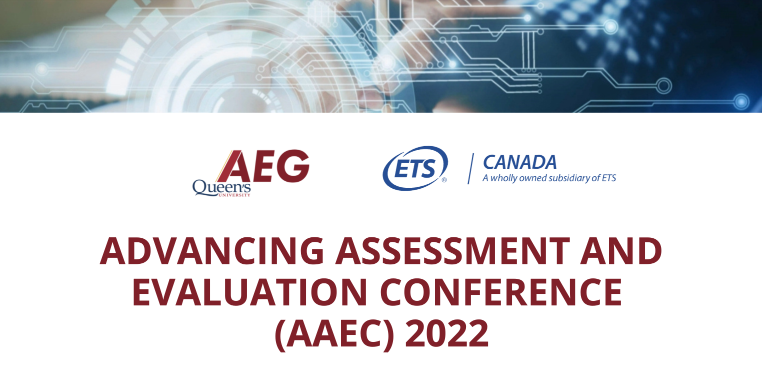
\includegraphics{Content/H.png}

\textbf{Description:} Advances in technology are too great to ignore. Assessment and evaluation practices in Canada appear to be lagging behind, when compared to other jurisdictions. This panel was designed to discuss recent technology advances in assessment and evaluation for possible use in Canada.

The following questions were intended to inspire and generate ideas. The speakers did not need to address the questions directly.

\begin{itemize}
\item
  What are the cutting edge technologies currently being used in assessment and evaluation?
\item
  What are the opportunities and challenges in taking advantage of these technological advances in learning and assessment?
\item
  With the technological advances where do you see the assessment and evaluation field in 5 years?
\item
  How can we begin to integrate more technology into everyday assessment and evaluation practices?
\end{itemize}

\newpage

\hypertarget{preparing-students-for-careers-focused-on-technology-based-assessment-and-evaluation}{%
\section{Preparing Students for Careers Focused on Technology-Based Assessment and Evaluation}\label{preparing-students-for-careers-focused-on-technology-based-assessment-and-evaluation}}

\textbf{Authors:} Mark J. Gierl, PhD \& Tahereh Firoozi

\textbf{Institution:} University of Alberta

\textbf{Recommended Citation:}

\begin{quote}
Gierl, M. \& Firoozi, T. (2022, January 27-28). \emph{Preparing Students for Careers Focused on Technology-Based Assessment and Evaluation} {[}Paper presentation{]}. Advancing Assessment and Evaluation Virtual Conference: Queen's University Assessment and Evaluation Group (AEG) and Educational Testing Services (ETS), Kingston, Ontario, Canada.
\end{quote}

We are at the beginning of data-enabled revolution. Massive amounts of data are produced every day. This data is collected using innovative software platforms and structured using advanced computational architectures so that machine learning algorithms can extract insights and yield outcomes that inform our decisions and guide our actions. This revolution is unfolding along two separate but related streams of research activity. The first stream is foundational research. Foundational research includes designing new data science, machine learning, and artificial intelligence methods and algorithms. It also includes developing appropriate computational platforms and software applications to implement these methods and algorithms. The second stream is applied research. Applied research implements the outcomes from the foundational research to solve practical problems in specific content areas. These content areas are not only different but also diverse, as they include fields that range from manufacturing to construction, health, energy technologies, and law enforcement, business to finance. Education is one of the applied content areas. Education will be profoundly affected by this data-enabled revolution. Educational measurement, research methodology, and evaluation now rely on data-mining techniques, machine learning algorithms, and learning analytic methods to analyze complex educational activities and outcomes, including cognitive, behavioural, and physiological (e.g., computer log files; eye tracking measures) data readily and abundantly generated by teachers and students. These techniques, algorithms, and methods are used to identify and to discover patterns and features that can be used, for instance, to predict learning outcomes, guide instructional methods, and inform curriculum developments. The information extracted from technology-based assessments will allow researchers and practitioners to create data-driven learning analytic models and applications to support learning and to guide teaching in digital learning environments that are becoming increasingly common as we begin the transition to an online educational world.

Unfortunately many of the programs that focus on educational measurement and evaluation in Canada---particularly at the graduate level---do not offer the kind of training that will enable students to contribute to either the primary or the secondary research stream guiding this data revolution. In fact, most students in educational measurement and evaluation have little training in data-mining techniques, machine learning algorithms, and learning analytic methods. Yet, these students will be expected to contribute to fields and areas of research or to compete for jobs and professions where these techniques, algorithms, and methods are already in place. Hence, we must quickly adapt our training programs to meet these changes and we must adjust our focus so that students become aware of and proficient in the techniques and methods that guide both the primary and secondary streams of research. In short, we must quickly adjust to the profound changes that are now occurring in the field of educational measurement and evaluation. These changes are motivated by the increased interest in and growing demand for extracting patterns and meaning from complex educational data sources that, increasingly, will guide evidence-based decision making throughout all levels in the educational system. We must therefore revise, augment, and update the focus of our programs in educational measurement and evaluation so that the students who complete their training can create, design, evaluate, and implement modern technology-based educational assessments along with the systems needed to support these assessments.

Every measurement and evaluation program in Canada is unique. Applied research areas within education are focused on many problems in a range of different contexts. Hence, a uniform training program is neither required nor desirable to prepare students for careers in measurement and evaluation. But we do feel that some guiding principles may be helpful. Hence the purpose of our paper is to identify and to describe three key principles that can be used to create programs to train the next generation of students in measurement and evaluation, particularly those graduate students who intend to focus on technology-enhanced assessment. For each principle, we describe the main idea behind the principle and then we describe how the principle can be implemented or supported within a program.

\textbf{PRINCIPLE 1 Interdisciplinary Focus:} Technology is developing concurrently in many fields and disciplines. Technology is also developing along two separate but related streams of research activity (i.e., foundational and applied). Students must understand both streams of research activity and, ultimately, how the streams are connected.

\begin{enumerate}
\def\labelenumi{\arabic{enumi}.}
\item
  Interdisciplinary coursework (i.e., coursework taken from Education, Computing Science, Electrical and Computer Engineering, Linguistics) for students is required to so different methods, perspectives, and standards of practice are infused in the students' program of study.
\item
  Recruiting students who have diverse educational backgrounds (i.e., students with backgrounds in Computing Science, Mathematics, Linguistics) and a wide range of experiences (i.e., students who have worked in industry prior to returning to graduate school) broaden the scope of a program for every faculty member and student because of the important benefits that are realized with the addition of different backgrounds, skills, research interests, and perspectives.
\item
  Graduate student committee representation should be interdisciplinary so different methods, perspectives, and standards of practice are infused in each student's program of research.
\item
  Faculty from different fields and disciplines should contribute to the outcomes in a program, with a focus on diverse but complementary research programs and teaching specializations.
\end{enumerate}

\textbf{PRINCIPLE 2 Flexible Program Delivery:} Shifts and changes in technology occur very quickly. As a result, programs must be flexible and must be capable of accommodating these constant changes. The purpose of offering a flexible program is to prepare students to be leaders in a rapidly changing world. The transition from a graduate program to a profession means that students must be proficient in using the latest techniques, algorithms, and methods.

\begin{enumerate}
\def\labelenumi{\arabic{enumi}.}
\item
  Multiple lines of focus in a program must be available because diverse applied research streams mean that different methods will be required to solve different types of problems. Student must therefore have many choices in the courses they complete---these choices should reflect the student's particular interests and should map onto a specific educational context. Hence, a flexible program in assessment and evaluation will have more elective than required courses.
\item
  Multiple lines of focus in a program must be available because diverse applied research streams mean that different methods will be required to solve different types of problems. Student must therefore have many choices in the research activities they pursue. Hence, a flexible program in assessment and evaluation will ensure that students can pursue diverse lines of research. This research agenda should include faculty supervision that resides both inside and outside of the program.
\item
  Students must have access to different kinds of technology-based resources to support their coursework and research. Some of these resources will only be available outside of the university environment (e.g., Google Cloud Platform; Amazon Cloud Computing).
\end{enumerate}

\textbf{PRINCIPLE 3 Culture for Creating Ideas:} Technology and innovation is driven by ideas. Hence, programs must cultivate a culture where faculty and students can work together to create and develop their ideas. Ideas develop in environments where creativity and risk are both valued and encouraged. Ideas also develop in environments that foster collaboration along with a healthy interplay between research and practice.

\begin{enumerate}
\def\labelenumi{\arabic{enumi}.}
\item
  Faculty members must initiate and maintain an active research program. The research program includes funding for graduate students.
\item
  A cohort model of student training is optimal where faculty attract highly-qualified students who can participate in their research program but also collaborate with other students and faculty in their program, in their university, and outside of the university.
\item
  Programs should strive to offer internships and to develop relationships with leaders in industry so students can develop their skills and see---first hand---the link between theory and practice, the benefits of collaborative research with practitioners in industry, and the importance of gaining experience in different working environments before making a career choice upon graduation.
\end{enumerate}

We predict that the data revolution will change the field of educational testing. The transition from paper- to computer-based tests almost guarantees our prediction will be realized because educators can now access tremendous amounts of data from students and teachers using online educational platforms and testing systems. The assessment and evaluation methods and techniques used in the past to model educational outcomes and to make educational inferences will become irrelevant. Fortunately, many new methods and techniques are either under-development or in-use to help us understand our increasingly data-focused world. It is important to ensure that students receive training that equips them to use these contemporary methods and techniques as well as contribute to the creation of new methods and techniques as the field of assessment and evaluation marches forward and, in the process, continues to change and evolve.

\newpage

\hypertarget{leveraging-technology-in-educational-measurement}{%
\section{Leveraging Technology in Educational Measurement}\label{leveraging-technology-in-educational-measurement}}

\textbf{Author:} Hollis Lai, PhD

\textbf{Institution}: University of Alberta

\textbf{Recommended Citation:}

\begin{quote}
Lai, H. (2022, January 27-28). \emph{Leveraging Technology in Educational Measurement} {[}Paper presentation{]}. Advancing Assessment and Evaluation Virtual Conference: Queen's University Assessment and Evaluation Group (AEG) and Educational Testing Services (ETS), Kingston, Ontario, Canada.
\end{quote}

It has been two decades into the 21st century. Educational assessment has experienced many hurdles in adopting new technologies. Computer-based testing, adaptive testing, automated scoring, and situational judgment tests are just a few of the innovations that are now in mass adoption. However, with the proliferation of interconnectedness through the internet and technology, there is an ever diverging skill set for the training of assessment and evaluation, and how to adopt it. To effectively leverage the use of technology in the field of educational measurement, I provide a summary of what is considered an expert in this field, what is training necessary for the field, and what are some actions needed for the field to leverage technology.

\textbf{1) What is an expert of educational measurement in the 21st century?}

To know what are the changes necessary to harness the change in technology, we must first reflect on what is deemed an expert of educational measurement today. A measurement expert today not only have to possess the traditional knowledge in measurement theory, test development, validity and standard-setting, but they must also be able to solve assessment issues of today such as addressing concerns of equity, diversity, and inclusiveness, provide strategies, and solve issues related to test security and cheating detection and provide advice and guidance to evolve testing practices that fit evolving requirements from the learners and the profession. Adding to this list of skills and knowledge, there is also a technical aspect of knowledge that is required such as understanding and implementing database queries, understanding information and software security paradigm, user experience and software design principles, and an understanding of various techniques in statistical and computational methods. In my humble experience with a decade of experience in medical education, I have noticed those are the skills that are commonly required in solving problems that are facing institutions and testing organizations. Suffice to say, the list is evolving and is becoming longer every day.

Testing practices are shifting in many disciplines. One such example in medicine is the adoption of competency-based training. This shift toward competency-based education has created: new opportunities to assess their learners, mobilization of many standard-setting panels, development of new assessment collection and reporting platforms, and new tools to facilitate and manage learner progression (these are the tools are the focus of my presentation). In this change, the experience for student training has evolved, how instructors determine learner competence has evolved, and the monitoring process of learners has evolved. However, this example of change management also highlighted some common themes that are occurring in other testing practices. First, expertise in measurement is required in developing and adapting to these changes, but in absence of educational measurement experts, the changes will continue. Second, the adoption of new technology and solutions can be low or high fidelity. Meaning, the adaptation of technology may not necessarily incur years of required development. Third, while educational measurement is still the kernel of most issues facing assessment and student learning, the measurement problem often requires an expert in measurement to identify this nuanced understanding. In sum, there are many interesting problems and opportunities to be solved in fields outside of educational measurement. It requires a well-rounded set of skills and understanding of all aspects of test development on a day-to-day basis.

\textbf{2) What are the skills needed in educational measurement in the coming decade?}

The knowledge, skills, and ability of educational measurement are evolving at an increasing pace. This is not unlike other fields of study, where an increasing number of skills are required at training to enter the field. There are three key attributes that I think will be needed for trainees of educational measurement entering into practice.

\emph{Technical Skills}

There is an increasing requirement for educational measurement to solve problems in the different domain spaces. Skills related to equating, survey and test development, latent scoring, statistical modelling and standard-setting are still needed, but they are stacked among other required understanding such as machine learning techniques, understanding of image and text processing approaches, and constraint programming approaches. A subset of these skills will help to solve the problems that are emerging in the next decade.

\emph{Problem Solving}

There is also a shift in the types of studies and research ongoing in educational measurement. Specifically, there is an increasing focus toward a problem-solving framework in presenting novel solutions in the field. In this shift, there are more and more applications and solutions from other fields of study that are being applied to problems in educational measurement. As the field of educational measurement evolves to incorporate issues in data and learning sciences, a problem-solving approach in studies may help in establishing a paradigm of knowledge.

\emph{Context Agnostic}

In educational measurement, learning needs to be captured at all levels of training. From early childhood education to the training of specialists, each stage or context of learning is different and requires different solutions in the evaluation of performance. Training in educational measurement should include the different nuances in each context but allow learners to apply their knowledge in an agnostic manner. Meaning, educational measurement experts should be well versed in the assessment of knowledge across all levels of learning. This is an important distinction as measurement experts in the upcoming decade will likely be adapting in different learning contexts, for training in different professions, languages and cultures, assessing skills and knowledge from learners with different backgrounds.

\textbf{3) How do we as a field leverage technology?}

Technology is an application of scientific knowledge into a field of practice. With educational measurement, the challenge of applying new technology is threefold: the ability to create the technology required in the field, the ability to adapt existing technology for use in the field, and the ability to persuade stakeholders in adapting the technology available. Experts and learners in educational measurement require a new skill set to create new technologies. Although machine learning and natural language processing techniques are skills in high demand, those are not the only skills required to leverage technology. Other fields of knowledge such as software architecture, cognitive sciences, design thinking, and user experience design can contribute to the creation of new technology to better facilitate and capture the measurement of learning. Learning and the evaluation of learning is a common task that is pervasive across many fields. By adapting paradigms and methods across different fields, the field of educational measurement can better leverage and improve our method of measurement for learning.

As experts in educational measurement, the development and adaptation of the new methods of assessment is an important role that will sustain the field. However, another role that is equally needed lies in knowledge translation of the new methods and technologies for assessments. This role requires an in-depth understanding of learning theories, arguments to validity, and communication. With an ever-increasing depth of knowledge in every field, being able to translate the theories and methods used for stakeholder understanding is a missing piece in translating theory into practice. Venues such as this one will help us communicate our background and be able to contribute to learning among a team of experts in computer, data, cognitive and statistical science.

In sum, my outlook remains positive in that education measurement is still needed while undergoing change. Our ability to adapt in a domain that requires knowledge in computer, data, cognitive, and statistical science relies on our ability to create and adapt new methods to improve the measurement of learning. Admittedly, the impact of the internet, social media, and the subsequent data revolution have created a demand to rationalize the burgeoning amount of data. It is now up to us, as experts in educational measurement, to design, prototype, validate, and implement solutions that fit our evolving need for assessment.

\newpage

\hypertarget{eqao-digitalization-of-large-scale-assessments}{%
\section{EQAO Digitalization of Large-Scale Assessments}\label{eqao-digitalization-of-large-scale-assessments}}

\textbf{Author:} Cameron Montgomery, PhD

\textbf{Organization:} Education Quality and Accountability Office (EQAO)

\textbf{Recommended Citation:}

\begin{quote}
Montgomery, C. (2022, January 27-28). \emph{EQAO Digitalization of Large-Scale Assessments} {[}Paper presentation{]}. Advancing Assessment and Evaluation Virtual Conference: Queen's University Assessment and Evaluation Group (AEG) and Educational Testing Services (ETS), Kingston, Ontario, Canada.
\end{quote}

The field of education has evolved considerably in recent years, increasingly incorporating digital learning tools. As an agency of the Government of Ontario mandated to assess students at key stages of their learning journey, the Education Quality and Accountability Office (EQAO) strives to continually improve its support of positive learning outcomes for all students. The agency quickly realised it needed to modernize its operations to reflect better the new fast-changing digital landscape. Digitalizing assessments ensures the agency continues to be responsive to the needs of the education community and that each student taking the assessment is offered the opportunity to demonstrate their understanding of the curriculum fully.

One of the challenges that faces large-scale assessment today is creating an assessment system where each test taker can fully demonstrate their knowledge and skills while the system maintains the reliability of data inherent to standardized testing. One digital assessment model, computer adaptive testing, reflects more accurately student achievement and the test taker's understanding of curricula and of what is being assessed. At this time, for its province-wide standardized assessments, the Education Quality and Accountability Office (EQAO) has adopted to use a Multi-Stage Computer Adaptive Testing (msCAT) model to assess mathematics, and a testlet-based Linear-on-the-Fly (tLOFT) model to assess literacy.

Digitalized large-scale assessments offer several opportunities compared to the paper-based assessment model formerly used by EQAO:

\begin{itemize}
\item
  Better alignment with the digital world that students engage with every day: In an age of rapid technological advancement, online assessments reflect both classroom and education experiences better.
\item
  Flexible assessment administration window: The computer assessment model allows for an assessment administration that can be available throughout the school year to support boards' and schools' schedules better. Schools and boards can administer large-scale assessments at their convenience to several groups of students at any time within the administration period.
\item
  Faster reporting: Computer assessments can offer immediate assessment results of multiple-select items upon completion by the student. Additionally, the remote online scoring of open-ended items is available at the scorer's schedule convenience and this allows the agency to engage with educators from across the province for all its scoring activities.
\item
  Inherent accommodations tools: Several accessibility tools are offered to every student through each assessment's toolbar.
\item
  Less carbon footprint: Digitalized assessments contribute to reducing waste connected to paper-based products.
\end{itemize}

At this juncture, the agency has identified some challenges linked to digitalized, online large-scale assessments:

\begin{itemize}
\item
  Unique information technology infrastructure of each school board: Ontario is a large province consisting of 72 boards and school authorities, each with its diverse technological needs, geography and system availability.
\item
  Device availability: There exists significant differences in the availability of in-person student devices in schools and boards. (This is being mitigated by offering longer administration windows that are opened from two to six months.) Additionally, the assessments need to be administered in-person for a specific group in a specific physical setting, and cannot be proctored remotely at this time.
\item
  New large-scale assessment process: Following the government's directive, the provincial assessments' online model and platform were developed and introduced rapidly after more than twenty years of administering paper-based assessments. EQAO needs to inform stakeholders in a very short time, and the agency continues to adapt learning modules aimed at administrators and other stakeholders as the online assessment initiative moves forward.
\end{itemize}

Equity is a key consideration in implementing digital assessments and it is important that the assessments be aligned with the everyday experiences of students. The technology should not be the driving force itself as it is the data and insights from the assessments that are paramount for system and student improvement. The agency's approach is anchored to being as flexible as possible and allowing schools to schedule the assessments at times that are suitable for them.

As the education and evaluation fields learn more about digital large-scale assessment platforms and as data become available for analysis, we can expect that technological advances will allow assessments in a few years to reflect student experiences much more accurately. Of particular note, assessments must continue to be responsive to the accessibility needs of each test taker, with a particular attention to increasing assessment customization and the inclusion of more accessibility tools. To engage students better as they are writing the assessment and help reduce stress associated with ``exams'', digital assessments will probably explore seriously the possibilities granted by gamification models.

\newpage

\hypertarget{using-text-mining-to-identify-authentic-content-neural-network-to-score-the-college-major-preference-assessment}{%
\section{Using Text Mining to Identify Authentic Content \& Neural Network to Score the College Major Preference Assessment}\label{using-text-mining-to-identify-authentic-content-neural-network-to-score-the-college-major-preference-assessment}}

\textbf{Authors:} Amery Wu, \textsuperscript{1}, Shun-Ful Hu, \textsuperscript{1}, \& Jacob Stone \textsuperscript{2}

\textbf{Institutions:} The University of British Columbia \textsuperscript{1}, Visier Inc.~\textsuperscript{2}

\textbf{Recommended Citation:}

\begin{quote}
Wu, A. D., Hu. S.F., \& Stone, J. E. (2022, January 27-28). \emph{Using Text Mining to Identify Authentic Content \& Neural Network to Score the College Major Preference Assessment} {[}Paper presentation{]}. Advancing Assessment and Evaluation Virtual Conference: Queen's University Assessment and Evaluation Group (AEG) and Educational Testing Services (ETS), Kingston, Ontario, Canada.
\end{quote}

\textbf{Background \& Purpose}

The traditional Psychometrics makes use of designed data for interpretation within the researchers' measurement/assessment framework. In contrast, Data Science and Artificial Intelligence have little interest in and dependence on a framework for interpretation. They use natural data to uncover patterns/algorithms for future prediction.

Computational Psychometrics, as a field, emerged from traditional Psychometrics in response to the variety, velocity, and volume of data obtained from the complex assessment systems made possible by new digital technology (von Davier, Mislevy, \& Hao, 2021). It incorporates devices from Data Science and Artificial Intelligence into traditional psychometric methodology.

This presentation reports two case studies of Computational Psychometrics utilizing the College Major Preference Assessment (CMPA, iKoda Research, 2017). The CMPA assists individuals in finding their top three favorites from 50 college majors that are commonly offered in Northern America. Case-1 used text mining techniques in Data Science to identify the CMPA assessment content. Case-2 used the multilabel neural network in machine learning to score a short version of CMPA with an aim to predict as well as the original version.

\textbf{Overview for CMPA}

The design of CMPA has two sections of different assessment formats in sequence: Likert-type rating and forced-choice. The Likert-type format is designed to narrow the 50 majors down to a list of candidates. The forced-choice format is designed to further nail down one's top three favorites. In addition, as a person progresses through the assessment, there are three steps at which the respondent's low scoring majors are screened out from any further assessment. This results in an adaptive test increasingly personalized to a respondent. The interpretation and use of the assessment results should only be personal. Wu (2021) reported good reliability and validity evidence for CMPA.

\textbf{Case-1: Using Text Mining Technique to Identify CMPA Assessment Materials}

To be as realistic and authentic as possible, the content of CMPA was extracted from the natural texts posted on the official websites. What follows describes the methods for creating the assessment content.

First, the corpus was gathered from the publicly available descriptions for courses that constituted a university major. Data was collected from over 40 Northern American Universities. The data collected for each major was compiled into a single very large document of raw text.

Then, we computed the term frequency-inverse document frequency (TF-IDF) for each document following the formula 𝑇𝐹-𝐼𝐷𝐹 = 𝑇𝐹 × 𝑙𝑛 (1/DF), where TF was the frequency of the term (word) in the document, and IDF was the inverse of the number of documents for the different majors in which the term appears (see Fan \& Qin, 2018). The TF-IDF yielded large values for words that appeared frequently in only one major but not others. This helped identify the ten most unique words for each major.

Next, we traced back to the original textual content to find the phrases that the ten terms were originally embedded in. For example, the term ``earthquake'' had a high TF-IDF for the document Geology, and it was embedded in phrases such as ``how earthquakes occur.''

This way, we identified phrases that best characterized the unique nature, activity, work, topic, and skills, associated with a major. These identified phrases were used as the basis for creating both the Likert-rating and forced-choice items. Other examples of the identified phrases are ``how the mind controls behaviour'' for Psychology and ``how plastic reacts when stressed'' for Material Sciences.

\textbf{Case-2: Using Neural Network to Score a Short Version of CMPA}

In machine learning, a neural network is a circuit of layers of artificial neurons, called nodes, connected by directional edges. The first layer is the input data, and the last layer is a set of nodes, each representing the predicted probabilities of different outcomes. The nodes are simply hidden (latent) variables that are a function of the nodes in the previous layer where the edges represent the weights. The goal of a neural network is to find the optimal structure, function, and weights for (i.e., train) the neural network based on the input data, so that it can produce the best outcomes for future predictions.

Case-2 used a supervised (labeled) machine learning technique of multilabel neural network to score the short version of CMPA. The short version consisted of only the first section, i.e., the 99 Likert items. As such, the neural network was regarded as a machine for scoring the 99 Likert items. If the scoring accuracy is satisfactorily high for all majors, it will be defensible to use only the short version to assess individuals' preference for the 50 majors, which is more time-efficient and less cognitively burdensome on the respondents.

Thus, the task of the multilabel neural network was to train the input data so that the short version could identify the top three majors for future users as effectively as the original longer version using the original summing-up scoring method. For each respondent, the trained network would output fifty probabilities (final scores), one for each major. To evaluate the prediction accuracy, the top three majors identified by the predicted probabilities were compared to the actual top three identified by the original CMPA procedure. Then, the proportion of agreement was taken as the accuracy rate. See Gargiulo, Silvestri, Ciampi, and De Pietro (2019) more explanation for multilabel neural network.

The results show that, with two middle layers, each with 64 nodes, the short version predicted the original outcomes exceedingly well. The minimum accuracy rate was 83\% for Philosophy, and the maximum accuracy rate was 99\% for Chemical Engineering, Electronic Engineering, and Materials Science. The overall accuracy had a median = 96\% and mean = 95\% across the 50 majors.

The results were highly generalizable to future users of CMPA. This was evaluated by a dataset different from training set that was saved for testing the generalizability of the trained multilabel neural network. The accuracy rates were almost equal to those reported in the last paragraph for the training data. The minimum accuracy rate was 81\% for Psychology and maximum accuracy rate was 99\% for Chemical Engineering, Electronic Engineering, and Materials Science. The overall accuracy had a median = 95\% and mean = 94\% across the 50 majors.

\textbf{Conclusion \& Future Work}

Both case studies showed that the techniques in Data Science and Artificial Intelligence, when used carefully with human judgement, can contribute to Psychometrics in a substantive way. That said, a frequent criticism on neural network is its black box approach to prediction because the algorithm for the prediction is entirely data driven and is often hard to make sense. This contradicts with the focus of psychometrics on explanation and evaluation. To tackle this problem, our future work will delve into how explanatory tools in Psychometrics can be beneficial to explanatory Artificial Intelligence, a field that helps to make sense how the input data contribute to the prediction.

As presented in a very recent book edited by von Davier et al.~(2021), there have been innovative examples of Computational Psychometrics. We anticipate more variety of marriages between Psychometrics and modern technology to create more exciting assessment projects.

\textbf{References}

Fan, H., \& Qin, Y. (2018, May). Research on text classification based on improved tf-idf algorithm. In X. Luo (Eds.) 2018 International Conference on Network, Communication, Computer Engineering (NCCE 2018) (pp.~501-506). Atlantis Press. doi: \url{https://doi.org/10.2991/ncce-18.2018.79}.

Gargiulo, F., Silvestri, S., Ciampi, M., \& De Pietro, G. (2019). Deep neural network for hierarchical extreme multi-label text classification. Applied Soft Computing, 79, 125-138.

iKoda Research (2017). Found a major you love. College Major Preference Assessment. Retrieved from: \url{https://www.i-koda.com/ikoda-college-website/}.

von Davier, A. A., Mislevy, R.J., Hao, J. Computational Psychometrics: New Methodologies for a New Generation of Digital Learning and Assessment. Methodology of Educational Measurement and Assessment (Eds.). Springer, Cham.

von Davier, A. A., Mislevy, R. J., Hao, J. (2021). Introduction to Computational Psychometrics: Towards a Principled Integration of Data Science and Machine Learning Techniques into Psychometrics. In: von Davier A.A., Mislevy R.J., Hao J. (Eds.) Computational Psychometrics: New Methodologies for a New Generation of Digital Learning and Assessment. Methodology of Educational Measurement and Assessment. Springer, Cham. \url{https://doi.org/10.1007/978-3-030-} 74394-9\_1.

Wu, S. (2021). Comparing Likert-type and forced-choice formats for assessing preference: a validation study on the College Major Preference Assessment (CMPA) {[}Master's thesis, University of British Columbia{]}. UBC Theses and Dissertation. Retrieved from \url{https://open.library.ubc.ca/collections/ubctheses/24/items/1.0397018}.

\newpage

\hypertarget{untitled}{%
\section{Untitled}\label{untitled}}

\textbf{Author:} Greg Roussel

\textbf{Organization:} Grand Erie District School Board

\textbf{Recommended Citation:}

\begin{quote}
Roussel, G. (2022, January 27-28). \emph{Untitled} {[}Paper presentation{]}. Advancing Assessment and Evaluation Virtual Conference: Queen's University Assessment and Evaluation Group (AEG) and Educational Testing Services (ETS), Kingston, Ontario, Canada.
\end{quote}

Advances in technology are too great to ignore. Assessment and evaluation practices in Canada appear to be lagging behind, when compared to other jurisdictions. This panel is designed to discuss recent technology advances in assessment and evaluation for possible use in Canada.

\textbf{What are the cutting-edge technologies currently being used in assessment and evaluation?}

The move to remote learning as a consequence of the COVID-19 pandemic has required many educators to adopt new skills and tools, including video conferencing, shared documents and digital spaces. Although these tools were available to educators in the Grand Erie District School Board prior to the pandemic, they were not widely used. Similarly, although the board implemented the learning management system Brightspace (see below), its usage was limited to the more technically savvy teachers, and teacher-consultants responsible for education technology. With the abrupt transition to remote learning in March of 2020 educators found themselves working in an unfamiliar context that required them to quickly learn and develop new skills for the effective use of these tools in remote teaching.

Brightspace is a promising learning management system that allows educators to interact with students in a digital space using a variety of tools such as:

\begin{itemize}
\item
  Posting assignments and rubrics
\item
  Creating small discussion groups and assignment spaces for students
\item
  Collecting completed work for assessment and evaluation
\item
  Allowing students to develop and maintain a portfolio of work to demonstrate learning
\end{itemize}

This interactive environment gives teachers and students the ability to share work and provide feedback in an asynchronous fashion. Features include:

\begin{itemize}
\item
  Teachers can post assignment rubrics ahead of time for students to reference.
\item
  Students can upload assignments
\item
  Teachers can provide feedback in a variety of ways, including notations in the document and a video response.
\item
  The Student Portfolio tool where students can provide evidence of their learning (e.g., a short audio clip explaining a concept, illustrations, notes) which teachers can use this evidence in their overall assessment.
\end{itemize}

One value-added feature of Brightspace is that it allows to teachers the ability to link specific expectations from the Ontario curriculum, which is available in the software, to an assignment. When evaluating the assignment, the teacher can see all the related expectations and assign the appropriate achievement level (Level 1, 2, 3, 4) for each expectation. For example, in Grade 9 Academic English an assignment may be designed to assess Reading for Meaning, with the specific expectation of \emph{Demonstrating Understanding of Content}; from the Ontario curriculum:

\begin{quote}
1.3 identify the important ideas and supporting details in both simple and complex texts (e.g., select details from a story to create a profile of a character in the story; use a graphic organizer to categorize the ideas in an article).
\end{quote}

Other tools in Brightspace include the ability to create online quizzes and surveys; set up small group discussions and assignment spaces as well checklists to help students navigate and manage the course.

\textbf{What are the opportunities and challenges in taking advantage of these technological advances in learning and assessment?}

The use of digital tools such as Brightspace provide tremendous opportunities for educators to meet students where they are, in terms of learning. Students today are ``digital natives'' and tend to possess highly developed technical skills that are more advanced than most adults. By reaching them on the devices that they use daily (phones, tablets, laptops) students can be more engaged in their learning. The asynchronous nature of digital spaces and remote learning allows students and teachers to engage with each other at times that are convenient for both.

The biggest obstacle in leveraging these technological advancements has been the slow uptake of new digital tools by educators. During the most recent provincial shutdown daily usage of Brightspace more than tripled at Grand Erie, suggesting that teachers are only using the tool during remote learning.

While some teachers are using Brightspace on a daily basis, it is only to take advantage of select tools. Teachers are predominately using the Assignments tool, by an almost 5:1 ratio compared to the next most popular tool, Quizzes. When looking at this phenomenon through the SAMR model (Substitution, Augmentation, Modification, and Redefinition) it is clear that most educators are still at the substitution or augmentation stage -- teachers are collecting assignments digitally versus paper.

While school boards have devoted funds to make technology available to all students the issue of equitable access is one that is not easily addressed. Many remote communities do not have broadband internet and families from lower socio- economic backgrounds do not have the financial resources to acquire the devices needed to access the technology.

\textbf{With the technological advances where do you see the assessment and evaluation field in 5 years?}

As a new, generation of teachers enter the classroom that have grown up with advanced educational tools we should expect that they will use technology in their assessment and evaluation practices more often. Given that most of the current technological usage is merely substituting paper for pixels there is hope that the next wave of teachers can move to modifying and redefining how these advances are used. The time that teachers will save using digital tools for assessments (administration and marking of assessments) will hopefully be directed to even more reflection on the individual student needs and relevant instruction for the different needs.

\textbf{How can we begin to integrate more technology into everyday assessment and evaluation practices?}

With the expectation of increased use of digital tools comes the requirement of increased training and support. It is not sufficient to provide teachers and educators with new digital tools with the expectation that they are implemented in the classroom. For effective and sustained use of technology, educators require ongoing support and training from the Ministry and school board administrations to see and explore the possibilities that are available for them in the classroom. It is also important to recognize how variable the digital capacity is of educators. This means training is going to require a tiered approach to meet the staff where they are. Ideally, this would also take advantage of digital technology with on-demand training to accommodate varying schedules and in-person and asynchronous opportunities to troubleshoot and share experiences.

\textbf{References}

Ontario Ministry of Education. (2007) The Ontario Curriculum Grades 9 and 10 English. Retrieved January 5, 2022 from: \url{http://www.edu.gov.on.ca/eng/curriculum/secondary/english910currb.pdf}

Romrell, D., Kidder, L. \& Wood, E. (2014). The SAMR Model as a Framework for Evaluating mLearning. Online Learning Journal, 18(2),. Retrieved January 5, 2022 from \url{https://www.learntechlib.org/p/183753/}.

\newpage

\hypertarget{discussant-summary-advancing-assessment-and-evaluation-by-leveraging-technology-perspectives-from-and-implications-for-research-practice-and-policy-in-a-rapidly-changing-world}{%
\section{Discussant Summary: Advancing Assessment and Evaluation by Leveraging Technology: Perspectives from and Implications for Research, Practice, and Policy in a Rapidly Changing World}\label{discussant-summary-advancing-assessment-and-evaluation-by-leveraging-technology-perspectives-from-and-implications-for-research-practice-and-policy-in-a-rapidly-changing-world}}

\textbf{Author:} Amanda Cooper, PhD

\textbf{Institution:} Queen's University

\textbf{Recommended Citation:}

\begin{quote}
Cooper, A. (2022, January 27-28). \emph{Advancing Assessment and Evaluation by Leveraging Technology: Perspectives from and Implications for Research, Practice, and Policy in a Rapidly Changing World} {[}Discussant Remarks{]} Advancing Assessment and Evaluation Virtual Conference: Queen's University Assessment and Evaluation Group (AEG) and Educational Testing Services (ETS), Kingston, Ontario, Canada.
\end{quote}

The COVID-19 pandemic has caused widespread school closures that has necessitated virtual learning at scale across K-12 education systems around the world. Consequently, education systems globally are grappling with rapidly changing virtual learning environments and the challenges surrounding leveraging technology to facilitate student learning. This theme explores advancing assessment and evaluation by levering technology and includes five panel members coming from different vantage points including universities, policymaking environments, and school districts. Knowledge mobilization (KMb) explores how research is applied and used to inform policy and practice in public service sectors. KMb utilizes a whole system perspective that explores three dimensions: research production (funders and universities), research use (practice and policymaking organizations like ministries of educations and school districts), and intermediary organizations that shape education systems (such as the Education Quality and Accountability Office in Ontario). I utilize KMb dimensions to explore the three vantage points offered by the diverse panelists --Research, Policy, and Practice -- in relation to advancing assessment and evaluation by leveraging technology in education.

\textbf{Contributors to Theme 2 Thought Papers}

\begin{itemize}
\item
  Dr.~Mark Gierl, Professor of Educational Psychology, Faculty of Education, University of Alberta
\item
  Dr.~Hollis Lai, Associate Professor, Faculty of Medicine and Dentistry, University of Alberta
\item
  Dr.~Cameron Montgomery, Chair, Education Quality and Accountability Office (EQAO), Ontario
\item
  Dr.~Amery Wu, Associate Professor, Faculty of Education, University of British Columbia
\item
  Greg Rousell, System Research Leader, Grand Erie District School Board
\item
  Discussant: Dr.~Amanda Cooper, Associate Professor of Educational Policy and Leadership and Associate Dean of Research, Faculty of Education, Queen's University
\end{itemize}

\textbf{Short Paper Summaries}

All five panelists describe the current context of technology and assessment in relation to rapid growth and development, including exponential growth of data across societal systems and virtual platforms. Drs. Gierl, Lai, and Wu explore technology and assessment in relation to research from university perspectives, whereas the final two panelists explore these issues from a policy perspective (Dr.~Montgomery) and a practice perspective (Rousell) within a school district.

\emph{Research}

Dr.~Gierl highlights that ``we are at the beginning of a data-enabled revolution'' (p.2). He outlines two separate but interrelated streams of research activity arising from this revolution:

\begin{enumerate}
\def\labelenumi{\arabic{enumi}.}
\item
  Foundational Research: ``Foundation research includes designing new data science, machine learning, and artificial intelligence methods and algorithms. It also includes developing appropriate computational platforms and software applications to implement these methods and algorithms''
\item
  Applied Research: ``Applied research implements the outcomes from the foundational research to solve practical problems in specific content areas. These content areas are not only different but also diverse, as they include fields that range from manufacturing to construction, health, energy technologies, and law enforcement, business to finance. Education is one of the applied content areas.''
\end{enumerate}

Dr.~Gierl outlines three key principles that are needed to train the next generation of students in measurement and evaluation: (1) Interdisciplinary, (2) Flexible Program Delivery, and (3) a Culture for Creating Ideas. Dr.~Gierl proposes an intriguing idea of ``creativity and risk'' for the field of educational testing to meet the needs of the data revolution and the changing landscape of assessment in the midst of technological advancement.

Dr.~Lai's paper begins by highlighting the historical hurdles the field of educational assessment has faced in adopting new technologies. He outlines assessment innovations such as computer-based testing, adaptive testing, automated scoring, and situational judgement tests that now have widespread adoption. He structures his paper around three questions: (1) What is an expert of educational measurement? (2) What skills are needed? (3) And how to leverage technology? The example of the shifts in medical education to competency-based medical training reflects some of the changing landscape of assessment of professional training programs. Dr.~Lai concludes his paper with a focus on LEARNING and the evaluation of learning as the common task and a unifying concept among disparate approaches, methods, and outcomes. Hollis suggests knowledge translation of new methods and technologies that are needed for assessment, alongside new skills and technologies for experts of educational measurement.

Dr.~Wu explores data science and artificial intelligence through two cases. Case 1 uses text mining techniques in data science to identify College Major Preference Assessment (CMPA) in 40 universities in North America. Case 2 uses multilabel neural network in machine learning to score a short version of the CMPA (99 Likert items). These approaches predicted outcomes exceedingly well with an overall accuracy across 50 majors (median 96\%, mean 95\%).

\emph{Policy and Practice}

Dr Montgomery's paper provides a policy perspective on large-scale assessment through an overview of the move to digitize EQAO (an intermediary organization that provides standards and implementation of literacy testing at scale across the province of Ontario). He outlines the benefits and challenges this year associated with a move to harness digital implementation of EQAO testing. Dr.~Montgomery highlights benefits of this approach including more flexible assessment window, faster reporting of instant results, less carbon footprint, and built in accessibility tools. However, he also highlights the challenges with changing EQAO in relation to uneven technological across the 72 school boards in the province, device availability in schools, and the capacity building needed to assist Principals and school leaders undertake this digitized assessment.

Greg Rousell, a system research leader from a school district, offers a much needed perspective from practice. He outlines the challenges of virtual learning and leveraging technology with teachers on the frontlines. His paper explores the use of Brightspace as a platform that offered a range of tools to teachers who all moved to virtual learning platforms during school closures for COVID-19. While students capacity for technology often rivals that of older generations (a realization that technological learning might prove to be more engaging for students), technological capacity of teachers is variable. Consequently, more work with educators and students is needed if school districts are to optimize the use of technology in assessment, and virtual learning more broadly.

\textbf{Implications and Future Questions}

The papers provoked ideas on how to leverage technology for assessment that varied depending on the vantage point from research, policy, or practice. I propose sparks for future thinking in relation to three areas: the good, the bad, and the unknown.

\emph{The Good}

\begin{itemize}
\item
  New possibilities: Technology is enabling things we might never have imagined in fields of assessment such as Artificial Intelligence, machine learning, and connecting global learners across dynamic platforms.
\item
  A Call for Interdisciplinarity and Collaboration: New research opportunities are emerging that encourage diverse collaboration across sectors which is improving our ability to solve complex social challenges
\end{itemize}

\emph{The Bad}

\begin{itemize}
\item
  Capacity-Building Needed: Capacity across sectors have not yet met the demand for the rapidly changing environment, as such investment is needed across the system for research producing organizations (universities) and research using organizations (schools)
\item
  Graduate Programs Must Become More Dynamic: In universities, need for new graduate programs -- more dynamic pathways, diverse committee structures that push boundaries of combining expertise of different fields
\item
  Schools: In school districts, technological and internet infrastructure is needed alongside training and capacity building for stakeholders
\item
  Policymaking: In governments and intermediaries, infrastructure and capacity building to meet the challenges of the digital age.
\end{itemize}

\emph{The Unknown}

\begin{itemize}
\item
  Equity remains an important concern across our public institutions especially in relation to education in relation to how technology influences learning outcomes, assessment and evaluation, among diverse groups
\item
  While many discuss the benefits of technology for Equity in relation to assessment, there is little discussion on how technology might contribute to widening gaps across various learners in our society and actually contribute to further inequities. These two areas are not mutually exclusive -- technology can offer positive contributions in some areas of equity, while simultaneously deepen these divides in other contexts.
\item
  More work is needed to explore how research, policy and practice are changing (or not) to meet the needs of a new era and how our public institutions can grapple with rapid and continual changes in technology.
\end{itemize}

\textbf{Conclusion}

As a scholar of knowledge mobilization and translation, I often talk about the connections between research, practice, and policy -- the push and pull of competing demands across large scale systems across diverse types of organizations and stakeholders. This panel and the diverse perspectives show that assessment and evaluation is a complex landscape involving diverse actors, organizations, and policies. As such, harnessing the benefits of technology to advance assessment will require alignment and collaboration across research systems, school systems, in conjunction with the policy landscape. In closing, I offer further questions to consider

\begin{enumerate}
\def\labelenumi{\arabic{enumi}.}
\item
  What role might policy play in harnessing technology for assessment from diverse vantage points in universities, government, and school districts?
\item
  What is the potential for ``creativity and risk'' (Gierl, 2022) in our public institutions?
\item
  What is the role of social innovation in advancing efforts to advance assessment by leveraging technology?
\item
  What potential exists to engage diverse actors to optimize these efforts, for instance, creating partnerships with industry?
\item
  What are the facilitators and barriers created by technology in assessment in relation to EDII?
\end{enumerate}

\newpage

\hypertarget{theme3}{%
\chapter{Promote Equity and Fairness}\label{theme3}}

\hypertarget{theme-overview-2}{%
\section{Theme Overview}\label{theme-overview-2}}

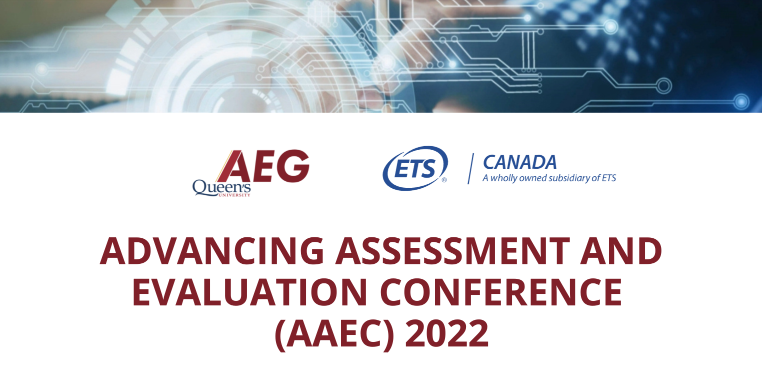
\includegraphics{Content/H.png}

\textbf{Description:} Assessment and evaluation are inexplicably linked to equity and fairness. Often assessment and evaluation are used to highlight or uncover issues of inequity. We asked panelists to consider the inverse, tasked with considering how advances in assessment and evaluation may come to promote equity and fairness.

The following questions were intended to inspire and generate ideas. The speakers did not need to address the questions directly.

\begin{itemize}
\item
  What can assessment and evaluation do to promote equity and fairness?
\item
  What can assessment and evaluation scholars do to promote equity and fairness?
\item
  How do equity, diversity, and inclusion influence the ways in which you approach assessment and evaluation?
\item
  How can we work with local partnerships as assessment and evaluation experts to promote equity and fairness?
\end{itemize}

\newpage

\hypertarget{understanding-a-trajectory-of-equity-in-evaluation-to-imagine-action-to-advance-equity}{%
\section{Understanding a Trajectory of Equity in Evaluation to Imagine Action to Advance Equity}\label{understanding-a-trajectory-of-equity-in-evaluation-to-imagine-action-to-advance-equity}}

\textbf{Author:} Michelle Searle, PhD, CE, OCT

\textbf{Institution:} Queen's University

\textbf{Recommended Citation:}

\begin{quote}
Searle, M. (2022, January 27-28). \emph{Understanding a Trajectory of Equity in Evaluation to Imagine Action to Advance Equity} {[}Paper presentation{]}. Advancing Assessment and Evaluation Virtual Conference: Queen's University Assessment and Evaluation Group (AEG) and Educational Testing Services (ETS), Kingston, Ontario, Canada.
\end{quote}

\textbf{Introduction and Positioning of the Author}

Advancing assessment and evaluation to promote equity and fairness is an important aspect of evaluators' theoretical and applied practice (Yarborugh, 2011). As an academic, researcher, and practitioner who is interested in the theory and practice of promoting the usefulness of evaluation, my values, and the work that I do positions me at the crux of embracing and embedding equity and fairness into both my scholarly and professional contributions to the field. Earlier in my career I lived internationally and worked as an educator. It was at this point when my perspective shifted, and I started thinking about equity and fairness as key elements in professional relationships and evaluative collaborations. Hall's (1976) iceberg idea of culture, recognizing the visible surface culture and how much deeper culture lies below is a good starting point for newcomers to this way of seeing the World. In thinking about the cultural iceberg, I hoped that by better understanding learners while engaging in integrative teaching, assessment, and evaluation, I could create a welcoming environment that prioritized taking risks and being courageous in our classroom community (Blackburn \& Niedzwiedz, 1980). In carrying these hopes and refining of my ideas for more than a I have become more aware that the links between culture and equity are rooted in systematic practices worthy of exploration (Zhou \& Fink, 2003). I believe evaluation is one-way practitioners and researchers can further explore to deepen their learning, increase their self-awareness, and hone their sensitivity.

To emphasize the value of the voices and experiences of others in my evaluation practice, research and teaching, I have prioritized collaborative (Roy \& Searle, 2020; Searle \& Poth, 2021; Searle et al., 2020; Shulha et al., 2019) and methodologically diverse evaluations (Searle, In Press) which regularly lead me to the inclusion of arts-informed inquiry (Cooper et al., In review; Searle, 2020; Searle \& Fels, 2018; Searle et al., 2016). In recent years, I have discovered that my efforts are insufficient. I am learning that we promote equity and fairness by questioning, surfacing assumptions and nourishing explicit communications. Including voices is different than intentionally centering the voices and experiences of others. Difficult conversations cannot be avoided (Katz \& Dack, 2012). In fact, few, if any aspects of evaluation are neutral, meaning that we cannot proceed as if they are (AEA, 2011). Thankfully, evaluation emphasizes the asking of questions, such as: who is being served by this program; who is experiencing barriers to access; what stories do people tell about the program; what biases do I hold as a listener; what do we need to learn/unlearn; and what data contributes to decision-making (Alkin, 2013). In asking these questions, evaluators including myself continue to unsettle evaluative assumptions in the pursuit of equity.

Many people are ready to commit to the idea of equity in evaluation, yet some may be wondering why we need to think about equity and fairness in evaluation now? The following three reasons are presented to answer why now:
1. Barriers to education and social programs affect groups based on gender, race, poverty, and many other factors (Hansman et al., 1999). Identifying and removing barriers supports equity (Schuelka et al., 2020). Equity is connected to cultural competence, making an understanding of culture necessary for understanding programs because programs and ``evaluations cannot be culture free'' (AEA, 2011). The field of evaluation considers cultural competence a requirement of a practicing evaluator (AEA, 2011; CES, 2018). By emphasizing cultural competence in the professionalization of the field, steps are being made to overcome barriers.

\begin{enumerate}
\def\labelenumi{\arabic{enumi}.}
\setcounter{enumi}{1}
\item
  In an equitable society all can prosper; the quality of education and access to social programs directly correlates to the development of children, youth, and adults (South et al., 2020). Evaluations help us understand and determine the quality of programming and make recommendations for improvement (Donaldson \& Picciotto, 2016). To promote an equitable society, we require equity-focused evaluations (Bamberger et al., 2016) and a willingness for evaluators to learn, change and act.
\item
  Finally, if not now, when? We are in the Decade of Evaluation for Action (Eval4Action, 2021). Evaluative thinking is in great demand globally by government, non-profits as well as the private sector, to determine the effectiveness of and contribute to ongoing learning related to, programs, policies, and practices. Therefore, now is the time to prioritize learning about and conducting equitable evaluations.
\end{enumerate}

When considering why the field of evaluation needs to focus on equity and fairness, the following section framed with four questions which reveal the trajectory of evaluation:

\begin{enumerate}
\def\labelenumi{\arabic{enumi}.}
\item
  How is the field of evaluation advancing with regard for equity and fairness?
\item
  In what ways can/does the practice of evaluation contribute to resolving issues of equity?
\item
  How do we strengthen the capacities of governments, organizations, and communities to evaluate with equity and fairness in mind?
\item
  What are considerations for moving forward with equity in evaluation?
\end{enumerate}

\textbf{How is the field of evaluation advancing with regard for equity and fairness?}

Shirin Ebadi wrote a story about rising female leadership which featured the quote, ``It is not just about hope and ideas. It's about action.'' Evaluators often embark on their journey in the field of evaluation with hopes and some ideas about equity and fairness (Robinson, 2011). But, action is the strength of evaluation. Program evaluation and research share many similarities, which are often summarized by Patton's adage (1997), ``Research seeks to prove; evaluation seeks to improve.'' Beyond this adage, evaluation is a human and contextual endeavour that acknowledges and incorporates differences in values and perspectives, focused on questions evaluands care about and aims to produce results for varied audiences including funders, program champions, participants, and the broader community or public (Alkin \& King, 2016; Ottoson \& Hawe, 2009; Rey et al., 2014). Evaluation, then, is about action which can influence positive outcomes in society (Gamble, 2008). The pandemic has brought to the forefront much information about racial and social unrest, challenged ideas about capitalism and awakened many to the need to act for a more equitable and fair society, a kind of social solidarity (Mishra \& Rath, 2020; Ray \& Rojas, 2020). Equity is related to the concept of being fair and impartial, promoting diversity and inclusion so that all people can participate and prosper (Bolino et al., 2008). Thinking about equity and evaluation is an invitation to think about what kinds of programs we have in education and society, and to examine the explicit ways these programs are pro-equity, prioritizing improving the conditions for groups with the greatest needs. Equity in evaluation includes a focus on the context in which the program operates, the power and people involved in programs (Donnelly, 2010; Bamberger \& Segone, 2011).

Promoting/Advancing equity and fairness in program evaluation poses challenges and opportunities (Patton, 2019). One challenge is understanding what evaluation is and if there are specific evaluation theories, approaches and methods that are better suited to advancing equity and fairness (Greene, 2005). Not surprisingly, program evaluation can be defined in many ways (Alkin and King, 2017). Early definitions of evaluation focused on the ``examination of worth, merit, or significance of an object'' (Scriven, 1998). This understanding of evaluation has expanded over time to include evaluations that are focused on establishing readiness, contribute to developing understanding, implementation, measuring effectiveness, and examining intended and unintended outcomes of programs (Mark, 2011). All evaluations focus on ``the systematic collection of information about the activities, characteristics, and outcomes of programs to make judgements about the program, improve program effectiveness, and/or inform decisions about future program development'' (Patton, 1997). Opportunity in evaluation lies in the expansions the field has undergone and its continued evolutions (Hogan, 2007; Shulha \& Cousins, 1997). The field of evaluation is known for its flexibility; in fact, we might consider evaluation as aligned with a growth-oriented mindset, because evaluation is often incorporating new approaches and methods for examining programs and contributing to transformation (Mertens, 2007). Many evaluators embrace their roles as capacity builders, innovators and change-makers who work alongside social champions to address complex challenges and use evidence for decision-making (Mertens, 2008).

\textbf{In what ways can/does the practice of evaluation contribute to resolving issues of equity?}

Evaluation is a relatively young field, which over recent decades has seen a growing emphasis on the role of stakeholders in evaluation (Hart et al., 2009). Stakeholders are defined by Greene (2005) as people who have a stake or a vested interest in the program, policy or product evaluated and therefore also have a stake in the evaluation. Stakeholder engagement was initiated to increase the utilization of evaluation (Greene, 1988). Ideas about stakeholder involvement in evaluation are captured in many evaluation approaches, including participatory (Cousins \& Earl, 1992), collaborative (Cousins \& Shulha, 2008; Shulha et al., 2016), democratic (House, 2000; Ryan, 2004), utilization-focused (Patton, 2008), empowerment (Fetterman, 2005), responsive (Stake, 2003), and transformative (Mertens, 2008) evaluations.

Stakeholder-engaged thinking and approaches have evolved over time about how, when and who to include in evaluation (Herremans et al., 2016). There is evidence to support that stakeholder approaches share advantages related to ``understanding, involvement, ownership, access, development, implementation, and improvement'' (Rodriguez-Campos, 2012). When thinking about equity, one important concept to remember is that there are many processes to engaging stakeholders, some might even consider it as a continuum of stakeholder engagement (Donnelly et al., 2016; Preskill \& Torres, 2000). An enduring message from the rise of stakeholder approaches is that stakeholders and communities are the experts in understanding and proposing solutions, therefore they are critical to promoting equity and fairness in evaluation (Brandon \& Fukunaga, 2014). Innovation in programs and evaluation is advanced through collaboration that enables co-learning (Matsumoto, 2018; Nsangi et al., 2020). Stakeholder-engaged approaches take time, commitment, and skills to work together, across differences and to envision unimagined possibilities (Svensson \& Cousins, 2015). Embracing equity and fairness through stakeholder-involved evaluation and research on evaluation is about working together as catalysts for change (Greene, 2005; Patton, 2019). Stakeholder-involved approaches are methodologically agnostic, meaning that they use the methods which are best suited to answer the questions stakeholders care about (Better Evaluation, 2021). This may include going beyond conventional quantitative or qualitative data collection, to engage in rich and robust data which can provide insight into complex social processes, attitudes, and experiences from those who were involved in the program as well as those who were not, or who may be hard to reach (Fetterman, 2017).

Innovative evaluation methodology that may support more equity and fairness through social change includes arts-informed inquiry using collage, poetic techniques, image-elicitation, and storytelling (Searle \& Shulha, 2016; Searle, 2020). Artful forms have a history of contributing to social change, just think of the work of Pablo Freire (1968 legendary poets such as Maya Angelou or Shane Koyczan and so many other artists who compel people to think, feel and see differently. There are also evaluators using the arts and researching the arts, recent CES members Jennica and Maya from ANDimplementation and past contributions from Eisner (1979), Goodyear (2007), Simons \& McCormack (2007) and MacNeil (2000), to name just a few. Artful approaches can contribute valuable perspectives that use multiple forms to create empathy and engage others in an experience (Barone \& Eisner, 2012). Providing access to these embodied experiences may evoke new understandings leading to improvement and change. The arts have the capacity to represent visibly and viscerally, it can uplift or challenge us, as pleasure, as inspiration and provocation (Searle \& Fels, 2018). The arts are already being used in evaluation; considering equity and fairness in evaluation is not about new techniques, it is about refocusing and refining the skills many evaluators already possess while enhancing the capacity of others.

\textbf{How do we strengthen the capacities of governments, organizations, and communities to evaluate with equity and fairness in mind?}

If we are to promote equity and fairness in our evaluations with the current demand for evaluators, then we must prioritize the examination of the practices used to teach evaluation, the partnerships formed to support evaluation and the collaborations that nourish evaluation mentorship (Christie et al., 2014; El Hassar et al., 2021; Poth \& Searle, 2021; Searle \& Poth, 2021). Higher education lacks sufficient evaluation learning opportunities rooted in evidence, particularly those centering experiential and community partnerships (Trevisan, 2002). We can both strengthen capacity and strengthen equity and fairness by developing interdisciplinary, cross-institutional, intersectoral and community-engaged projects (e.g., Armitage \& Levac, 2015).

One way to actively strengthen the capacity of evaluation education and the reach of evaluation courses, is to engage in teaching collaboratives. I am a partner in a teaching collaborative that is entering its second with Dr.~Gokiert at the University of Alberta. The catalyst for this partnership between us as scholars and evaluators as well as our academic institutions was developing an intensive experiential evaluation course. This course was established by Mignone (2018) and later adapted as UEval by Gokiert with colleagues (Gokeirt et al., 2021). The inaugural joint version of the course was offered in the Spring of 2021 and was called, UEval/QEval. This course leverages our skills, perspectives, and networks by addressing and investigating evaluation learning, while building student and participant evaluation capacity through experiential and community-engaged research (Davis \& MacKay, 2014; Gokiert et al., 2021; Preskill \& Boyle, 2008; Reed, 2015). In this course, research and teaching are used to link students, staff, and scholars to issues of policy and practice across sectors by partnering with community organizations with a social imperative. The equity seeking aims of these community partner groups might include a focus on sexual health programming, community-police relationships, serving newcomers, offering programs for students at risk or addressing food and housing insecurities. Recently the idea of launching this program at Queen's was recognized and has received funding as an education-leadership opportunity (\url{https://www.queensu.ca/gazette/stories/announcing-first-education-leaders-residence}). By continuing the first interdisciplinary co-learning partnership with students and communities across institutions and examining the efficacy of this model, the Assessment and Evaluation Group at Queen's University contributes to ``reimagining our relationship'' (p.~5) and placing equity as a central goal (Deane, 2020).

\textbf{What are the/some considerations for moving forward with equity in evaluation?}

The pathway for a more just society is strengthened when the capacity for evaluation and research on evaluation are furthered through collaborations, embracing diverse knowledge, and working reciprocally with communities (Gokiert et al., 2017). Positioning evaluation and research on evaluation as promoting a more just society involves harnessing processes and tools to further understand impact-driven practices for advancing understanding and community change (Reed et al., 2015).

It's inspiring to be an evaluation scholar right now, with access to strong mentors, fantastic collaborators, and dedicated students (Gullickson et al., 2019). As poet Frost (1922) proclaimed, ``promises to keep. And miles to go before I sleep''. This quote might prompt evaluators to pause to recognize that we have a lot to be grateful for, especially as we are on this road together, interested in understanding and committing to action for advancing equity in evaluation. The list below helps translate some of the ideas from this paper into actions for evaluation researchers and practitioners alike:

\begin{enumerate}
\def\labelenumi{\arabic{enumi}.}
\item
  Examine intentionality of self, in others as well as in programs, policies, and practices.
\item
  Engagement matters. Prioritize developing collaborations and nourish inclusion.
\item
  Promote interdisciplinarity. Come prepared to learn/unlearn as each other's teachers.
\item
  Embrace complexity with a creative mindset that enables you to stay engaged through difficulties.
\item
  Imagine and act through a lens of methodological humility and flexibility.
\end{enumerate}

The list consolidates some of my ideas and hopes for how evaluators can begin to take action toward advancing equity and fairness in our work. Remembering the Ebadi quote from earlier that urged us to action, I must clarify: my action, in evaluation and in research on evaluation, is through learning and promoting the learning of others. Not surprisingly, I reflect that my learning is a work in progress, as I continue thinking about theories and practices that support equity and practical suggestions or tools that I can adopt. For now, I offer Table 1 for a not-so-exhaustive draft of my evaluation commitments and practical actions. As you review my evaluation commitments and actions, I ask you to consider what are your commitments and considerations to advancing equity?

\textbf{Commitments and Considerations for Advancing Equity and Fairness in Evaluation}

\emph{Commitments as an evaluator and researcher of evaluation who is advancing equity:}

\begin{itemize}
\item
  Continue to be knowledgeable about emerging evaluation theory, approaches, and methods
\item
  Stay informed about program evaluation standards, guiding principles and competencies
\item
  Engage often in reflexive practice to recognize power, privilege, and bias (e.g., build reflectivity into planning, establish prompts, use multiple processe)
\item
  When considering a project, engage in community-scoping to gain a more in-depth understanding of a community, its social diversity, history, networks, and characteristics
\end{itemize}

\emph{Considerations for evaluation partners/client/collaborators to act for advancing equity:}

\begin{itemize}
\item
  Examine intentionality to see intended and unintended consequences; use a wide lens for looking at influences and impacts of projects, not just the specific project objectives.
\item
  Explicitly frame evaluation questions to allow for or promote the exploration of equity issues that may have arisen in a context.
\item
  Assess readiness for evaluation to promote equity by engaging in context/environmental scanning, document analysis and/or asset inventory.
\item
  Use logic modelling or theory of change processes to be explicit about values and assumptions, question the logic through courageous conversations.
\item
  Conduct a power analysis by asking whose knowledge and evidence is likely to be overlooked unless we make an explicit effort to include them? Hear from those not included to ask why didn't they access, use, or participate in the program?
\item
  Disseminate learning broadly and engage in reflection systematically.
\end{itemize}

\textbf{References}

Alkin, M. C. (Ed.). (2013). Evaluation roots. Thousand Oaks, CA: Sage.

Alkin, M. C., \& King, J. A. (2016). The historical development of evaluation use. American Journal of Evaluation, 37(4), 568-579.

American Evaluation Society. (April 22, 2011). American Evaluation Association Statement on Cultural Competence in Evaluation. \url{https://www.eval.org/Community/Volunteer/Statement-on-Cultural-Competence-in-Evaluation}

Armitage, T., \& Levac, L. (2015). Th e development of community-engaged scholars through course-based learning: A student perspective. Engaged Scholar Journal: Community Engaged Research, Teaching and Learning, 7 (1), 148--163.

Barone, T., \& Eisner, E. W. (2012). Arts based research. Thousand Oaks, CA: SAGE Publications.

Bamberger, M., Raftree, L., \& Olazabal, V. (2016). The role of new information and communication technologies in equity-focused evaluation: Opportunities and challenges. Evaluation, 22(2), 228-244.

Bamberger, M., \& Segone, M. (2011). How to design and manage equity-focused evaluations. New York: UNICEF Evaluation Office.

Better Evaluation. (2022, January 24). Understand and engage stakeholders. \url{https://www.betterevaluation.org/en/rainbow_framework/manage/understand_engage_stakeholders}

Blackburn, J. D., \& Niedzwiedz, E. (1980). Do Teaching Methods Matter: A Field Study of an Integrative Teaching Technique. Am. Bus. LJ, 18, 525.

Bolino, M. C., \& Turnley, W. H. (2008). Old faces, new places: Equity theory in cross‐cultural contexts. Journal of Organizational Behavior: The International Journal of Industrial, Occupational and Organizational Psychology and Behavior, 29(1), 29-50.

Brandon, P. R., \& Fukunaga, L. L. (2014). The state of the empirical research literature on stakeholder involvement in program evaluation. American Journal of Evaluation, 35(1), 26-44.

Canadian Evaluation Society. (2018). Competencies for Canadian evaluation practice. Retrieved from \url{http://www.evaluationcanada.ca/txt/2_competencies_cdn_evaluation_practice.pdf}

Christie, C. A., Quiñones, P., \& Fierro, L. (2014). Informing the discussion on evaluator training: A look at evaluators' course taking and professional practice. American Journal of Evaluation, 35(2), 274-290.

Cousins, J. B., \& Earl, L. M. (1992). The case for participatory evaluation. Educational evaluation and policy analysis, 14(4), 397-418.

Davis, R. S., \& MacKay, K. (2014). Evaluator training: Content and topic valuation in university evaluation courses. American Journal of Evaluation, 35 (3), 419--429.

Donaldson, S. I., \& Picciotto, R. (Eds.). (2016). Evaluation for an equitable society. IAP.

Donnelly, J. (2010). Maximising participation in international community-level project evaluation: A strength-based approach. Evaluation Journal of Australasia, 10(2), 43-50.

Donnelly, C., Shulha, L., Klinger, D., \& Letts, L. (2016). Using program evaluation to support knowledge translation in an interprofessional primary care team: A case study. BMC Family Practice, 17(1), 1-14.

Eisner, E. W. (1979). The use of qualitative forms of evaluation for improving educational practice. Educational Evaluation and Policy Analysis, 1(6), 11-19.

El Hassar, B., Poth, C., Gokiert, R., \& Bulut, O. (2021). Toward an evidence-based approach to building evaluation capacity. Canadian Journal of Program Evaluation, 36(1).

Eval4Action. (2022, January 24). Decade of Evaluation for Action. \url{https://www.eval4action.org}

Fetterman, D. M., \& Wandersman, A. (Eds.). (2005). Empowerment evaluation principles in practice. Guilford Press.

Fetterman, D. M., Rodríguez-Campos, L., \& Zukoski, A. P. (2017). Collaborative, participatory, and empowerment evaluation: Stakeholder involvement approaches. Guilford Publications.

Freire, Pablo. (1968). Plan de trabajo. Paz y tierra. Rio de Janeiro. P.25

Frost, R. (1922). The Witch of Coos. Poetry, 19(4), 175-181.

Gamble, J. A. A. (2008). A developmental evaluation primer. JW McConnell Family Foundation, Canada.

Gokiert, R. J., Kingsley, B. C., Poth, C., Edwards, K., El Hassar, B., Tink, L. N., Tremblay, M., Cor, K., Springett, J., \& Hopkins, S. (2017). Developing an evaluation capacity building network in the fi eld of early childhood development. Engaged Scholar Journal: Community-Engaged Research, Teaching, and Learning, 3 (2), 59--79.

Gokiert, R. J., Daniels, J., Brazil, J., Pittman, S., Poth, C., Karbabian, A., \ldots{} \& Jun, S. (2021). UEval: Bringing Community-Based Experiential Learning to the Evaluation Classroom. Canadian Journal of Program Evaluation, 35(3).

Goodyear, L. K. (2007). Poetry, performance and pathos in evaluation reporting. In Dilemmas of engagement: Evaluation and the new public management. Emerald Group Publishing Limited.

Greene, J. G. (1988). Stakeholder participation and utilization in program evaluation. Evaluation review, 12(2), 91-116.

Greene, J. C. (2005). A value‐engaged approach for evaluating the Bunche--Da Vinci Learning Academy. New Directions for Evaluation, 2005(106), 27-45.

Gullickson, A. M., King, J. A., LaVelle, J. M., \& Clinton, J. M. (2019). The current state of evaluator education: A situation analysis and call to action. Evaluation and Program Planning, 75, 20--30.

Hall, E. T. (1976). Beyond Culture. Garden City, NY: Anchor Press.

Hart, D., Diercks-O'Brien, G., \& Powell, A. (2009). Exploring stakeholder engagement in impact evaluation planning in educational development work. Evaluation, 15(3), 285-306.

Hansman, C. A., Spencer, L., Grant, D., \& Jackson, M. (1999). Beyond diversity: Dismantling barriers in education. Journal of instructional psychology, 26(1), 16.

Herremans, I. M., Nazari, J. A., \& Mahmoudian, F. (2016). Stakeholder relationships, engagement, and sustainability reporting. Journal of business ethics, 138(3), 417-435.

Hogan, R. L. (2007). The historical development of program evaluation: Exploring past and present. Online Journal for Workforce Education and Development, 2(4), 5.

House, E. R., \& Howe, K. R. (2000). Deliberative democratic evaluation. New directions for evaluation, 85, 3-12.

Katz, S., \& Dack, L. A. (2012). Intentional interruption: Breaking down learning barriers to transform professional practice. Corwin Press.

MacNeil, C. (2000). The prose and cons of poetic representation in evaluation reporting. American Journal of evaluation, 21(3), 359-367.

Mark, M. M. (2011). Toward better research on---and thinking about---evaluation influence, especially in multisite evaluations. New Directions for Evaluation, 2011(129), 107-119.

Matsumoto, C., (2018). Advantages of increasing evaluation capacity in nonprofits. (Unpublished master's thesis). The University of Minnesota.

Mertens, D. M. (2007). Transformative paradigm: Mixed methods and social justice. Journal of mixed methods research, 1(3), 212-225.

Mertens, D. M. (2008). Transformative research and evaluation. Guilford press.

Mishra, C., \& Rath, N. (2020). Social solidarity during a pandemic: Through and beyond Durkheimian Lens. Social Sciences \& Humanities Open, 2(1), 100079.

Mignone, J., Hinds, A., Migliardi, P., Krawchuk, M., Kinasevych, B., \& Duncan, K. A. (2018). One room school: The Summer Institute in Program Evaluation. The Canadian Journal of Program Evaluation, 33 (2), 268--278.

Nsangi, A., Oxman, A. D., Oxman, M., Rosenbaum, S. E., Semakula, D., Ssenyonga, R., \ldots{} \& Sewankambo, N. K. (2020). Protocol for assessing stakeholder engagement in the development and evaluation of the Informed Health Choices resources teaching secondary school students to think critically about health claims and choices. PloS one, 15(10), 1--15 (2020).

Ottoson, J. M., \& Hawe, P. (2009). Editors' notes. New Directions for Evaluation, 2009(124), 3-5.

Patton M, Q. (1997). Utilization-focused evaluation: The new century text. Sage Publications.

Patton, M. Q. (2008). Future trends in evaluation. From policies to results: Developing capacities for country monitoring and evaluation systems. Paris: UNICEF and IPEN, 44-56.

Patton, M. Q. (2019). Blue marble evaluation: Premises and principles. Guilford Publications.

Poth, C., \& Searle, M. (2021). Competency-Based Evaluation Education: Four Essential Things to Know and Do. Canadian Journal of Program Evaluation, 35(3).

Preskill, H., \& Boyle, S. (2008). A multidisciplinary model of evaluation capacity building. American Journal of Evaluation, 29(4), 443-459

Preskill, H., \& Torres, R. T. (2000). The learning dimension of evaluation use. New Directions for Evaluation, 2000(88), 25-37.

Ray, R., \& Rojas, F. (2020). Inequality during the coronavirus pandemic. Context's blog.

Reed, R., King, A., \& Whiteford, G. (2015). Re-conceptualising sustainable widening participation: evaluation, collaboration, and evolution. Higher Education Research \& Development, 34(2), 383-396.

Rey, L., Tremblay, M. C., \& Brousselle, A. (2014). Managing tensions between evaluation and research: illustrative cases of developmental evaluation in the context of research. American Journal of Evaluation, 35(1), 45-60.

Robinson, S. B. (2011). Inside, outside, upside down: Challenges and opportunities that frame the future of a novice evaluator. New Directions for Evaluation, 2011(131), 65-70.

Rodríguez-Campos, L. (2012). Advances in collaborative evaluation. Evaluation and program planning, 35(4), 523-528.

Roy, S., \& Searle, M. (2020). Scope Creep and Purposeful Pivots in Developmental Evaluation. Canadian Journal of Program Evaluation, 35(1).

Ryan, K. E. (2004). Serving public interests in educational accountability: Alternative approaches to democratic evaluation. American Journal of Evaluation, 25(4), 443-460.

Searle, M. J., \& Shulha, L. M. (2016). Capturing the imagination: Arts-informed inquiry as a method in program evaluation. Canadian Journal of Program Evaluation, 31(1).

Searle, M., \& Fels, L. M. (2018). An artistic contemplative inquiry: What arrives in co-contemplating assessment and evaluation. Artizein: Arts and Teaching Journal, 3(1), 12.

Searle, M. J., Kirkpatrick, L. C., Smyth, R. E., Paolini, M., \& Brown, H. M. (2020). Promoting Learning Through a Collaborative Approach to Evaluation: A Retrospective Examination of the Process and Principles. In Collaborative Approaches to Evaluation: Principles in Use. Sage Publishing

Searle, M. (2020). Enhancing Educational Decision-Making: Arts-Informed Inquiry as a Feature of Collaborative Evaluations. In Perspectives on Arts Education Research in Canada, Volume 2 (pp.~76-96). Brill.

Searle, M., \& Poth, C. (2021). Collaborative evaluation designs as an authentic course assessment. Canadian Journal of Program Evaluation, 35(3).

Schuelka, M. J., Braun, A. M., \& Johnstone, C. J. (2020, January). Beyond access and barriers: Inclusive education and systems change. In FIRE: Forum for International Research in Education (Vol. 6, No.~1).

Shulha, L., \& Cousins, J. B. (1997). Evaluation use: Theory, research, and practice since 1986. Evaluation Practice, 18, 195--208.
Shulha, L. M., Whitmore, E., Cousins, J. B., Gilbert, N., \& al Hudib, H. (2016). Introducing evidence-based principles to guide collaborative approaches to evaluation: Results of an empirical process. American Journal of Evaluation, 37(2), 1-23.

Shulha, L. M., Searle, M., Poth, C. N., \& Chalas, A. (2019). Stakeholders weigh in on collaborative approaches to evaluation. Growing the Knowledge Base in Evaluation: The Contributions of J. Bradley Cousins, 99

Simons, H., \& McCormack, B. (2007). Integrating arts-based inquiry in evaluation methodology: Opportunities and challenges. Qualitative Inquiry, 13(2), 292-311.

South, E. C., Butler, P. D., \& Merchant, R. M. (2020). Toward an equitable society: building a culture of antiracism in health care. The Journal of Clinical Investigation, 130(10), 5039-5041.

Stake, R. (2003). Responsive evaluation. In International handbook of educational evaluation (pp.~63-68). Springer, Dordrecht.

Svensson, K., \& Cousins, J. B. (2015). Meeting at the crossroads: Interactivity, technology, and evaluation utilization. Canadian Journal of Program Evaluation, 30(2), 143-159.

Trevisan, M. S. (2002). Evaluation capacity in K-12 school counseling programs. American Journal of Evaluation, 23(3), 291-305.

Yarbrough, D.B., Shulha, L.M., Hopson, R.K., \& Caruthers, F.A. (2011). The program evaluation standards: A guide for evaluators and evaluation users (3rd. ed). Corwin Press.

Zhou, A. Z., \& Fink, D. (2003). The intellectual capital web: a systematic linking of intellectual capital and knowledge management. Journal of intellectual capital.

\newpage

\hypertarget{without-recognition-of-student-childrens-rights-equity-in-assessment-falls-flat-and-short}{%
\section{Without Recognition of Student (Children's) Rights, Equity in Assessment Falls Flat and Short}\label{without-recognition-of-student-childrens-rights-equity-in-assessment-falls-flat-and-short}}

\textbf{Author:} Jacqueline P. Leighton, PhD

\textbf{Institution:} University of Alberta

\textbf{Recommended Citation:}

\begin{quote}
Leighton, J. (2022, January 27-28). \emph{Without Recognition of Student (Children's) Rights, Equity in Assessment Falls Flat and Short} {[}Paper presentation{]}. Advancing Assessment and Evaluation Virtual Conference: Queen's University Assessment and Evaluation Group (AEG) and Educational Testing Services (ETS), Kingston, Ontario, Canada.
\end{quote}

\textbf{Introduction}

Twenty-five years ago, my attention centered on measurement models and tools, with significantly less attention on student learning. Over the course of 25 years, the focus of my attention has flipped. My research and advocacy in student assessment in the past decade now focus on children's human rights within the classroom; this includes not only assessment but also all pedagogical activities associated to learning in the classroom. Two broad approaches guide my research: (1) the United Nations Convention on the Rights of the Child (UN, 1989) and (2) the third force of psychology - humanistic psychology (Rogers, 1969).

\textbf{Pragmatic Perspective}

My entry point into children's human rights came from the observations I made while working within K-12 schools; in particular, my observation that children often have very little say or voice in matters relevant to their best interests (Leighton, 2020, 2021; UN, 2009). This relative absence of participation may be rooted in outdated conceptions of children, their socio-emotional development, and their positions as rights holders. Outdated conceptions of children may undergird the types of relationships teachers develop with students. Two of the largest teacher education programs in Canada -- Alberta and Ontario -- have no formal instruction in the UNCRC (Leighton, 2022). In other words, many teachers are relatively unaware of their responsibilities as duty bearers vis-à-vis children. Thus, the student-teacher relationship, which I label the pedagogical alliance, plays a pivotal role in this research and, as such, there can no longer be any separation of assessment from teaching and learning in the research I conduct. The economic, educational, and psychological research base that shows the influence of teachers in the experience and outcomes of students is simply too robust to avoid.

The perspective that the UNCRC provides is pragmatic since it is a legally-binding international agreement. All countries have ratified the UNCRC except the United States. The UNCRC involves 4 core principles (Lundy \& Byrne, 2017):

\begin{itemize}
\item
  No child shall be subjected to discrimination.
\item
  Practices taken shall be in the best interest of the child.
\item
  Children shall freely express their views and participate in matters that pertain to them.
\item
  All children shall be supported in their healthy development and survival.
\end{itemize}

Although the UNCRC is not rooted in any one theoretical perspective, it has the backing of significant research in children's mental and physical health. Thus, the UNCRC is primarily a data driven document, the upshot being that use of the UNCRC requires a strong commitment to high-quality data. Any and all interventions developed and administered to facilitate children generally and their learning in particular must be rigorously implemented and evaluated using high quality research designs and samples.

\textbf{Research Focus}

A focus on children's human rights cannot be a partisan political undertaking if the best interest of all students is the goal. It is for this reason that I avoid the term equity in my research and writings. This term is over-used in my view, without clear behavioral definition, and has become more of a dogmatic statement that an evidence-based pathway to better student assessment and learning. Although a simple definition of equity is the practice of being fair and impartial, many educational institutions (including universities) have adopted practices under the term `equity' that may be characterized as prejudicial (e.g., eliminating programs for certain groups of students); such practices can harm more than benefit students. Indeed, the effects of equity practices should be the basis of rigorous study and debate but this has not occurred; probably because practices adopted are more political than educational.

Consequently, in an effort to bring rigor and avoid dogma, my research involves children's human rights and how assessments and student-teacher relationships can be improved to benefit all students. As per the UNCRC, the research aims to not privilege any one group of children based on gender, race, ethnicity, socioeconomic background, ability, religion or gender orientation. This means that in studies of how assessments ought to be designed, administered and interpreted, what guides the work is what is in the best interest of children irrespective of their particular backgrounds, identities or injustices previously suffered.

\textbf{Food for Thought}

This research program makes particular demands on those who undertake it. At the outset is the need to avoid simple solutions to complex problems in an effort to correct previous wrongs in the lives of children. This means putting dogma aside and doing what we, as researchers have been trained to do, gather data and engage in the best interpretation of the results. Moreover, the focus has to be on children and students and less so on the political leanings of adults. For example, in a book I recently finished titled Leveraging Socio-Emotional Assessment to Foster Children's Human Rights (2022), the entire last chapter is devoted to the collective failure on the part of many governments, public health officials, academics and teachers' unions in understanding and rectifying the failure of COVID policies on children's development and learning.

\textbf{References}

Leighton, J.P. (2022). Leveraging Socio-Emotional Assessment to Foster Children's Human Rights. Part of the Student Assessment for Educators (Book Series Editor - J. McMillan). Oxfordshire, UK: Routledge (Taylor \& Francis Group).

Leighton, J.P. (2021). Not all that counts is safe for counting: Barriers to collecting learning data for assessment purposes. In R. Lissitz and H. Jiao (Eds.), Enhancing effective instruction and learning using assessment data. Information Age Publishing.

Leighton, J.P. (2022). A study of teacher candidates' views on children's human rights in Canada. International Journal of Children's Rights.

Leighton, J.P. (2020). On barriers to accessing children's voices in school-based research. Canadian Journal of Children's Rights, 7(1), 164-193.

Leighton, J.P. (2020). Cognitive diagnosis is not enough: The challenge of measuring learning with classroom assessments. In S.M. Brookhart \& J.H. McMillan (Eds.), Classroom assessment and educational measurement (pp.~27-45). NCME Book Series. Routledge.

Lundy, L., \& Byrne, B. (2017). The four principles of the United Nations convention on the rights of the child: The potential value of the approach in other areas of human rights law. In Brems, E., Desmet, E., \& Vandenhole, W. (Eds.), Children's rights law in the global human rights landscape (pp.~52-70). Taylor \& Francis Group.

Rogers, C. (1969). Freedom to learn: A view of what Education might become. Columbus, Ohio: Charles E. Merrill.

The United Nations. (1989). Convention on the Rights of the Child. Treaty Series, 1577, 3.

UN Committee on the Rights of the Child. (2009, July 20). General comment No.~12: The right of the child to be heard. Retrieved Dec 1 2019 at \url{https://www2.ohchr.org/english/bodies/crc/docs/AdvanceVersions/CRC-C-GC-12.pdf}

\newpage

\hypertarget{fairness-and-inclusion-on-canadas-large-scale-assessments}{%
\section{Fairness and Inclusion on Canada's Large-scale Assessments}\label{fairness-and-inclusion-on-canadas-large-scale-assessments}}

\textbf{Authors:} Tess Miller, PhD \& Elizabeth Blake

\textbf{Institution:} University of Prince Edward Island

\textbf{Recommended Citation:}

\begin{quote}
Miller, T. \& Blake, E. (2022, January 27-28). \emph{Fairness and Inclusion on Canada's Large-scale Assessments} {[}Paper presentation{]}. Advancing Assessment and Evaluation Virtual Conference: Queen's University Assessment and Evaluation Group (AEG) and Educational Testing Services (ETS), Kingston, Ontario, Canada.
\end{quote}

\hypertarget{abstract}{%
\subsection{Abstract}\label{abstract}}

The purpose of this thought paper was to highlight the interplay of inclusive education and large-scale assessment exclusion rates drawing into question the fairness of having students with diverse learning needs participate in large-scale assessments. The idea and data for this paper was drawn from three studies examining exclusion rates in Canada and a literature review on issues related to inclusive education. Melding these two issues revealed an explanation for high exclusion rates.

\newpage

\hypertarget{thought-paper}{%
\subsection{Thought Paper}\label{thought-paper}}

A review of national and international LSA scores for Canadian students over the past four cycles of administration revealed inconsistent and high rates non-participants (Miller \& Yan, n.d.). The high percentage of students not participating in LSAs exceeds the 5\% cap articulated in the PISA technical standards (CMEC, 2016). For example, when examining the number of non-participants on the national Pan-Canadian Assessment Program (PCAP) for mathematics, that is, students who were excluded because of a disability or limited language, students who were absent on the day of the assessment, and students who were excluded under a category PCAP described as other (i.e., a category which provides discretion for school administrators not to include students in the assessment), the number of non-participants on the mathematics assessment was over 25\% in the province of Prince Edward Island (PE) and Nova Scotia (NS). On the next administration of the PCAP assessment of mathematics in 2016, the number of non-participants for British Columbia (BC) and NS was over 20\% (Miller \& Yan, n.d.). An examination of non-participants on the Programme for International Student Assessment (PISA) was similar to patterns on the PCAP where over 27\% of students from PE could be classified as non-participants on the 2015 assessment of mathematics (CMEC, 2016). The number of non-participants is so alarming that Anders et al.~(2021) questioned whether Canada's education system was worth of the laurels it has been bestowed. It is important to note that this surge in the percent of non-participants is not just a Canadian phenomenon as similar findings have been reported in the US and UK (Anderson, Lai, Alonzo \& Tindal, 2011; Braun, Zhang \& Vezzu, 2010; Jerrim, 2021). Hence the purpose of this thought paper is to pose an explanation for what has been called a selection bias on LSAs.

We posit that the high rate of non-participants may indeed be a selection bias but the root of the problem is connected to theories of inclusive education. Prior to the 1990s, children with intellectual and physical disabilities were segregated from mainstream classrooms. One family challenged this and the outcome of the Supreme Court of Canada ruled that disabled children had every right to attend their local school with their same age peers (Moore v. British Columbia, 2012). Exclusion rates from LSAs during the early 2000s still were still low and below the 5\% cap. Following the court ruling in 2012, the practice of inclusive education became more widespread resulting in classrooms with a more diverse set of learners. At the same time, definitions of inclusive education continued to broaden which resulted in greater diversity in the classroom. A typical classroom has evolved to include students with many special needs such as behaviour (e.g., inattention, impulsivity), academic (e.g., dyslexia, dyscalculia), and socio-emotional (e.g., anxiety). This resulted in a greater demand for learning and accommodation resources which unfortunately, did not accompany the policy on inclusion. Thus, it is likely that students requiring additional support fall through the gaps due to a lack of resources and are left to flounder in the public education system. It is highly possible that these students are not operating a grade level. As students are passed from one grade to the next due to a practice of social promotion where students are promoted to the next despite having met grade level outcomes (Robertson, 2021), students fall further and further behind.

When students become of age to write the PCAP (i.e., 13-year-olds) and PISA (15-year-olds), school administrators ponder the fairness of deciding who should write the LSA and who should not (Miller \& FitzGerald, 2022). Although the definition of disability is not entirely clear (Anderson et al, 2011; McGill et al., 2016), there is a distinction between students who have a psychological disability (e.g., schizophrenia, manic depression) versus a learning disability. Based on the current PCAP and PISA exclusion guidelines, students with intellectual disabilities can be excluded; however, given the diversity of learners in the inclusive classroom, it is likely that students with learning needs (not disabilities) are also being exempted as school administrators claim it is not fair to require a student operating a grade or more below grade level, complete a LSA that they have not been prepared to write (Miller \& FitzGerald, 2022).

A closer look at the composition of classrooms and the learning needs of children in the classroom is needed to affirm this theory. In the event this theory is proven correct, LSA administrators may need to revisit their policies in light of inclusive education practices and prepare guidelines clearly articulating who should write the LSA and who should not to ensure LSA scores are reflective of the student population being measured.

\textbf{References}

American Psychological Association (2020). What is intellectual disability. Retrieved from \url{https://www.psychiatry.org/patients-families/intellectual-disability/what-is-intellectual-disability}

Anders, J., Has, S., Jerrim, J., Shure, N., \& Zieger, L. (2021). Is Canada really an education superpower? The impact of non-participation on results from PISA 2015. Educational Assessment, Evaluation and Accountability, 33, 229--249. \url{https://link.springer.com/content/pdf/10.1007/s11092-020-09329-5.pdf}

Anderson, D., Lai, C. F., Alonzo, J., \& Tindal, G. (2011). Examining a grade-level math CBM designed for persistently low-performing students. Educational Assessment, 16(1), 15--34.

Braun, H., Zhang, J., \& Vezzu, S. (2010). An investigation of bias in reports of the National Assessment of Educational Progress. Educational Evaluation and Policy Analysis, 32 (1), 24--43.

CMEC. (2016). Measuring up: Canadian results of the OECD PISA 2015 study. Retrieved from \url{https://www.cmec.ca/Publications/Lists/Publications/Attachments/389/PISA2015_CPS_EN.pdf}

Jerrim, J. (2021). PISA 2018: How representative is the data for England and Wales? Retrieved from \url{https://ffteducationdatalab.org.uk/2021/04/pisa-2018-how-representative-is-the-data-for-england-and-wales/}

Miller, T. \& Yan, Y. (n.d.). Factors Influencing the Accuracy of Canada's Large-scale Assessment Data: Policies and practices of exclusion, absenteeism, and social promotion

Miller, T. \& FitzGerald, A. M. (2022). The practice of excluding students from large-scale assessments: Interviews with principals, Alberta Journal of Educational Research.

Miller, T. \& Yankey, A. (n.d.). The practice of excluding students from large-scale assessments: The perspectives of mathematics teachers {[}Unpublished manuscript{]}. University of Prince Edward Island

OECD. (2015a). PISA 2018 technical standards. Retrieved from \url{https://www.oecd.org/pisa/pisaproducts/PISA-2018-Technical-Standards.pdf}

OECD. (2015b). Sample Design. Retrieved from \url{https://www.oecd.org/pisa/sitedocument/PISA-2015-Technical-Report-Chapter-4-Sample-Design.pdf}

OECD. (2017). PISA 2015 Technical Report. Retrieved from \url{http://www.oecd.org/pisa/sitedocument/PISA-2015-technical-report-final.pdf}

OECD. (2019). PISA 2018: Insights and Interpretations. Retrieved from \url{https://www.oecd.org/pisa/PISA\%202018\%20Insights} \%20and\%20Interpretations\%20FINAL\%20PDF.pdf

Roberts, R. M. (2021). To retain or not retain: A review of literature related to kindergarten retention. Retrieved from \url{https://eric.ed.gov/?id=ED611006}

Supreme Court of Canada (2012), Moore v. British Columbia (Education), SCC 61 (CanLII).

\newpage

\hypertarget{assessing-non-cognitive-skills-to-promote-equity-and-academic-resilience}{%
\section{Assessing Non-Cognitive Skills to Promote Equity and Academic Resilience}\label{assessing-non-cognitive-skills-to-promote-equity-and-academic-resilience}}

\textbf{Authors:} Louis Volante, PhD \textsuperscript{1} \& Don A. Klinger, PhD \textsuperscript{2}

\textbf{Institutions:} Brock University \textsuperscript{1} ; University of Waikato \textsuperscript{2}

\textbf{Recommended Citation:}

\begin{quote}
Volante, L. \& Klinger, D. (2022, January 27-28). \emph{Assessing non-cognitive skills to promote equity and academic resilience} {[}Paper presentation{]}. Advancing Assessment and Evaluation Virtual Conference: Queen's University Assessment and Evaluation Group (AEG) and Educational Testing Services (ETS), Kingston, Ontario, Canada.
\end{quote}

\textbf{Acknowledgement:}

This research is supported by the Social Sciences and Humanities Research Council of Canada (SSHRC)

\textbf{Introduction}

The global pandemic has created undeniable hardships for school-aged children, teachers, and parents around the world. Understandably, governments and policymakers are concerned about the impact of COVID-19 on student learning and achievement. This concern is mirrored in the emerging research, which has used large-scale assessment measures to attempt to quantify the degree of `learning losses' that students have experienced as a result of school closures, shifts towards online and hybrid learning, and other impacts associated with successive waves of this deadly virus. Not surprisingly, this body of research suggests that learning stalled during the pandemic, with the greatest impacts felt by at-risk student populations, such as those with lower socio-economic status (SES) and migrant backgrounds (see Engzell et al., 2021; Kaffenberger, 2021; Maldonato \& De Witte, 2021).

Discussions of student progress, or lack thereof, have also been examined alongside the construct of academic resilience. While defined in numerous ways, academic resilience is typically considered to be present in those children who obtain positive achievement outcomes despite being disadvantaged due to factors such as lower SES or facing adversity. As one example, for the purposes of cross-national comparisons, the Organisation for Economic Cooperation and Development (OECD) defines disadvantaged youth as those in the lowest one-third of its socioeconomic indicator within each country, based on information about parents' occupation(s) and along with measures of household possessions (OECD, 2018a). Countries which possess smaller achievement gaps between high and low-SES student populations are said to be more equitable and also more successful in promoting academic resilience (Agasisti, et al., 2018).

\textbf{Cognitive vs.~Non-Cognitive Skills}

Notwithstanding concerns about critical learning losses, the COVID-19 pandemic has also forced us to reconsider the relative importance ascribed to cognitive versus non-cognitive skills, an admittedly problematic albeit common distinction. International standardized tests such as the OECD's Programme in International Student Assessment (PISA), as well as national large-scale assessment programs, have been fairly adept at measuring cognitive skills such as reading, mathematics, and science literacy. The OECD has also begun to measure and report on non- cognitive skills such as growth mindset and socio-emotional issues (Kautz, 2014; OECD, 2018b). Yet it is worth noting that measures such as PISA occur on a triennial basis and are based on cross-sectional data. Additionally, PISA focuses only on students who are approximately 15-years of age. Cross-sectional data based on single age cohorts are limited in that they do not allow for the examination and comparisons of different age groups and stages of development over time (Volante \& Klinger, in press).

One might naturally query how governments are positioned to respond to shocks such as COVID-19 in the absence of more timely and robust data -- particularly in light of the troubling mental health and general wellness patterns that have recently emerged. For example, a recent study conducted by the Hospital for Sick Children in Ontario, Canada found approximately 70 percent of children/adolescents experienced deterioration in at least one of six mental health domains during the pandemic: depression, anxiety, irritability, attention, hyperactivity, or obsessions/compulsions (Cost et al., 2021). Similarly, a survey of the impact of COVID-19 found less than 5 percent of Canadian children 5--11 years old and 0.6 percent of youth 12--17 years old were meeting required physical activity guidelines (Moore et al., 2020). Collectively, these findings underscore the deleterious effects of the pandemic and the need to consider broader notions of resilience for school-aged populations.

\textbf{Toward a Broader Conceptualization of Academic Resilience}

Contemporary studies suggest a broader conceptualization of academic resilience is required that extends beyond mere measures of learning losses in student populations. Our proposed triarchic model (see Volante et al., 2021), expands the nature and scope of considerations policymakers should examine when gauging academic resilience, both during and post-COVID by focusing on three key areas:

\begin{itemize}
\tightlist
\item
  \emph{Academic Supports:} Policies, procedures, and/or guidelines that support students' academic success.
\item
  \emph{Physical Health Supports:} Policies, procedures, and/or guidelines that support students' physical health and well-being.
\item
  \emph{Mental Health Supports\_:} Policies, procedures, and/or guidelines that support students' mental health.
\end{itemize}

\textbf{Innovative Assessment Designs}

Along with the need for a broader conception of academic resilience, there is also a need for more innovative and timely large-scale measures that can assess the three key areas of resilience we have identified above: academic supports; physical health supports; and mental health supports. The foundations for such measures are already in place at international and national levels. The OECD has long been interested in health and well-being outcomes, and the International Association for the Evaluation of Educational Achievement (IEA) has recently developed the Responses to Educational Disruption Survey (REDS), which is focused on the impact of the pandemic. Further the Health Behaviour of School-Aged Children survey (HBSC) (e.g., Craig, King, \& Pickett, 2020; Inchley, Currie, Budisavljevic, Torsheim, Jåstad, Cosma, et al., 2020) has over 30 years of data on children's health. There was a previous effort from the OECD to incorporate the HBSC survey into its PISA cycle. There are also examples of large- scale surveys focused on various aspects of childrens' health and wellbeing used by provincial governments in Canada.

Nevertheless, these measures are typically independent of each other, resulting in potential duplication of surveys but with survey designs that are not fully compatible. Using Canada as an example, provincial surveys can often be linked to individual students through student identification numbers. In contrast, international assessments do not link their data to individual students. On the other hand, international survey instruments tend to be larger and their items and constructs have been carefully researched and validated, something national and provincial organisations are unable to duplicate due to resources. Lastly, international assessments tend to follow at multiyear cycle, providing a broad estimate of shifts over time, while the annual nature of provincial assessments and surveys are more responsive to recent shifts in learning or health impacts.

The current pandemic has highlighted the challenges of measuring the impact of major events on the educational and health outcomes of our children. While governments desire reliable, valid, and timely data to guide their decisions regarding the education and health of our children, our current measures are largely unable to do so. As a result, we need to create more interdependent assessments that incorporate the sampling methods of provincial assessments and surveys along with the survey tools developed by international organisations such as the OECD, the IEA, and the HBSC. This would enable us to obtain longitudinal data about specific cohorts of students on well-defined measures of educational outcomes related to health, well-being, and resilience.

To reiterate, there are already examples of this in place. The Canadian team of HBSC researchers have worked closely with the Public Health Agency of Canada and with provincial and territorial governments to produce specific reports focused on the interests of these provinces and territories. It may already be too late to provide accurate information of the initial impact of COVID-19 on our children. Yet the ongoing challenges the pandemic continues to create serve to highlight the necessity of focusing our efforts to monitor its effects on children's education and health. Ultimately, the proposed assessment reforms are meant to assist governments and policymakers in their efforts to promote equity and academic resilience.

\textbf{References}

Agasisti, T., et al.~(2018). Academic resilience: What schools and countries do to help disadvantaged students succeed in PISA. OECD Education Working Papers, No.~167. OECD Publishing. \url{https://doi.org/10.1787/e22490ac-e}

Cost et al.~(2021). Mostly worse, occasionally better: Impact of COVID-19 pandemic on the mental health of Canadian children and adolescents. European Child Adolescent Psychiatry. \url{https://pubmed.ncbi.nlm.nih.gov/33638005/}.

Engzell, P., Frey, A., \& Verhagen, M. D. (2021). Learning loss due to school closures during the COVID-19 pandemic. Proceedings of the National Academy of Sciences of the United States of America, 118(17), 1-7. \url{https://www.pnas.org/content/pnas/118/17/e2022376118.full.pdf}.

Craig, W. M., King, M., \& Pickett, W. (2020). The Health of Canadian Youth: Findings from the Health Behaviour in School-aged Children Study. Public Health Agency of Canada. \url{https://www.canada.ca/content/dam/phac-aspc/documents/services/publications/science-research-data/hbsc/health-behaviour-school-aged-children-study-report.pdf}

Inchley, J., Currie, D., Budisavljevic, S., Torsheim, T., Jåstad, A., Cosma, A., et al., editors (2020). Spotlight on adolescent health and well-being. Findings from the 2017/2018 Health Behaviour in School-Aged Children (HBSC) survey in Europe and Canada. International report. Volume 1. Key findings. Copenhagen: WHO Regional Office for Europe. \url{https://www.euro.who.int/en/health-topics/Life-stages/child-and-adolescent-health/health-} behaviour-in-school-aged-children-hbsc/publications/2020/spotlight-on-adolescent-health-and- well-being.-findings-from-the-20172018-health-behaviour-in-school-aged-children-hbsc-survey- in-europe-and-canada.-international-report.-volume-1.-key-findings

Kaffenberger, M. (2021). Modelling the long-run learning impact of the Covid-19 learning shock: actions to (more than) mitigate loss. International Journal of Development, 81. \url{https://www.sciencedirect.com/science/article/pii/S0738059320304855\#}

Kautz, T., et al.~(2014). Fostering and Measuring Skills: Improving Cognitive and Non- Cognitive Skills to Promote Lifetime Success. OECD Publishing. www.oecd.org/education/ceri/Fostering-and-Measuring-Skills-Improving-Cognitive-and-Non-Cognitive-Skills-to-Promote-Lifetime-Success.pdf

Maldonato, J. E., \& De Witte, C. (2021). The effect of school closures on standardised student test outcomes. British Educational Research Journal. \url{https://doi.org/10.1002/berj.3754}

Moore et al.~(2020). Impact of the COVID-19 virus outbreak on movement and play behaviours of Canadian children and youth: A national survey. International Journal of Behaviour Nutrition and Physical Activity, 17. \url{https://doi.org/10.1186/s12966-020-00987-8}

Organisation for Economic Cooperation and Development. (2018a). Equity in Education: Breaking Down Barriers to Social Mobility. OECD Publishing. www.oecd.org/education/equity- in-education-9789264073234-en.htm

Organisation for Economic Cooperation and Development. (2018b). PISA 2018 Results (Volume III). OECD Publishing. www.oecd-ilibrary.org/education/pisa-2018-results-volume- iii\_bd69f805-en

Volante, L., \& Klinger, D. (in press). PISA, global reference societies, and policy borrowing: The promises and pitfalls of `academic resilience'. Policy Futures in Education.

Volante, L., Klinger, D., \& Barrett, J. (2021). Academic resilience in a post-COVID world: A multi-level approach to capacity building. Education Canada, 61(3), 32-34. \url{https://www.edcan.ca/articles/academic-resilience-in-a-post-covid-world/}

\newpage

\hypertarget{discussant-summary}{%
\section{Discussant Summary}\label{discussant-summary}}

\textbf{Author:} Chi Yan Lam, PhD, CE

\textbf{Independent Scholar}

\textbf{Recommended Citation:}

\begin{quote}
Lam, C. Y. (2022, January 27-28). \emph{Discussant Summary} {[}Discusssant Remarks{]}. Advancing Assessment and Evaluation Virtual Conference: Queen's University Assessment and Evaluation Group (AEG) and Educational Testing Services (ETS), Kingston, Ontario, Canada.
\end{quote}

Good afternoon! Thank you for having me here.

Let me start off by expressing my sincere thanks and appreciation to the panelists for their illuminating and inspiring thoughts on advancing assessment and evaluation to promote equity and fairness.

At no point in our recent history are issues of equity and fairness more prominent in both academic and public discourse than now. The pandemic has laid bare inequities in our social institutions, from education and health to our justice system and our economy (e.g., Chen \& Bougie, 2020; Ismail, Tunis, Zhao, \& Quach, 2021; Khare, Shroff, Nkennor, Mukhopadhyay, 2020; Perry, Aronson, \& Pescosolido, 2021; Whitley, Beauchamp, \& Brown, 2021). And increasingly, we're realizing that much of these inequities are not only a condition of the present but also part of the design of our institutions of our past (e.g., Holton, 2021). For these reasons, I find this session timely, needed, and essential as we envision a tomorrow that could be different and better than one we have today.

My name is Chi Yan Lam. I am a public sector evaluator. In that role, I work with both internal and external evaluators to design, commission, and implement large-scale evaluations of government programs. In turn, I work with policy advisors and policymakers on improving programs and designing new policy interventions. But I'm not here in the capacity as a public servant but as a member of the academy. For the past ten years, I've have been working with students at the Faculty of Education and the Faculty of Health Sciences, Queen's University on honing their assessment and evaluation knowledge and skills as a term adjunct. So, it is through this dual lens of policy and scholarship that I will discuss these papers.

Let me begin by offering brief observations about each of these papers before concluding with remarks.

Professor Searle. I really enjoyed your paper for its personal, reflective, and reflexive stance. I was moved by your commitment to examining the self in relation to evaluation theory/practice. It is this critical stance that I wish more practitioners and scholars would adopt.

Professor Leighton. Your paper stood out to me for its strong commitment to inviting scholars to adopt explicit frameworks in their attempts to promote equity and fairness. You reminded us that in the debate of equality versus equity that individual needs are what is ought to be at the forefront of policy considerations--- ``person, not boxes''.

Professor Miller. Your paper with Professor Blake on exclusion highlighted that the stories that we tell of our educational systems are a function of who gets to participate in the construction of those stories.

And Professor Volante. Your paper with Professor Klinger on broadening conceptualization of academic resilience is noteworthy and, of course, timely for its explicit intent in stimulating further dialogue among policymakers in their efforts to promoting equity and academic resilience.

Now, let me now offer some remarks.

One of the consistent through lines across this set of papers was their desire to speak to policymakers and seek influence in the public sphere. As someone who straddles both worlds---that of policy and the academy---I can tell you that policymakers do listen, and ideas do percolate\ldots{} but that process can be slow, and that policymakers' bandwidths are often consumed by political priorities and the issue of the day. So, my two invitations to you are to: (1) continue to find ways to mobilize your ideas in a digestible format, even at the risk of being reductive. (One way to accomplishing that might be to post the key ideas of your paper in under five bullets, on one slide, on your web site, so that a policy advisor could more readily draw on these ideas when preparing policy materials.); and (2), to continue to building that rationale for promoting equity and fairness---but in a way that relates it to the goals of our educational systems in both pragmatic (in the here-and-now sense) and fundamental fashions (in terms of the society we wish to build collectively.) It is through these levers that I could see academics as having greater influence over policy discourse.

For my second remark, I'd like to turn to the notion of allyship. The act of allyship occurs when a person of privilege works in solidarity and partnership with those in lesser power to help take down systems that challenge those being disadvantaged and oppressed (Washington \& Evans, 1991). So, in the context of our current focus, I would invite all of us to consider expanding how you think about the audiences of your work to building in ideas for how allies could support and further the work of equity and fairness in assessment and evaluation. Put simply, what could allies take away from your work. On this note, I tip my hat to Prof.~Leighton whose paper had introduced the notion of pedagogical alliance between that of student and teacher.

And finally, it strikes me as important to point out that one of the common roots which underpin both assessment and evaluation is the construction of merit: what counts as meritorious in learning, programs, curriculum, and policies---and more importantly, who gets to say what counts as meritorious in what study. So, my invitation to all is to look beneath the surface of what we study to questioning the values systems which underpin our inquiry.

In closing, I thank our panelists for their papers on this very important topic. They've highlighted that while we have much to celebrate in our educational systems, much work remains. And today, we've taken another important step towards shaping a society that could be more equitable, fair, and just.

Thank you.

\textbf{References}

Chen, I., \& Bougie, O. (2020). Women's Issues in Pandemic Times: How COVID-19 Has Exacerbated Gender Inequities for Women in Canada and around the World. Journal of Obstetrics and Gynaecology Canada, 42(12), 1458.

Holton, W. (2021). Liberty is Sweet: The Hidden History of the American Revolution. Simon \& Schuster.

Ismail, S. J., Tunis, M. C., Zhao, L., \& Quach, C. (2021). Navigating inequities: a roadmap out of the pandemic. BMJ Global Health, 6(1), e004087.

Khare, N., Shroff, F., Nkennor, B., \& Mukhopadhyay, B. (2020). Reimagining safety in a pandemic: the imperative to dismantle structural oppression in Canada. CMAJ, 192(41), E1218-E1220.

Perry, B. L., Aronson, B., \& Pescosolido, B. A. (2021). Pandemic precarity: COVID-19 is exposing and exacerbating inequalities in the American heartland. Proceedings of the National Academy of Sciences, 118(8).

Washington, J., \& Evans, N. J. (1991). Becoming an Ally. In N. J. Evans \& V. A. Wall (Eds.), Beyond tolerance: Gays, lesbians and bisexuals on campus (pp.~195--204). American Association for Counseling and Development.

Whitley, J., Beauchamp, M. H., \& Brown, C. (2021). The impact of COVID-19 on the learning and achievement of vulnerable Canadian children and youth. Facets, 6(1), 1693-1713.

\newpage

\hypertarget{Theme4}{%
\chapter{Promote Language Learning}\label{Theme4}}

\hypertarget{theme-overview-3}{%
\section{Theme Overview}\label{theme-overview-3}}

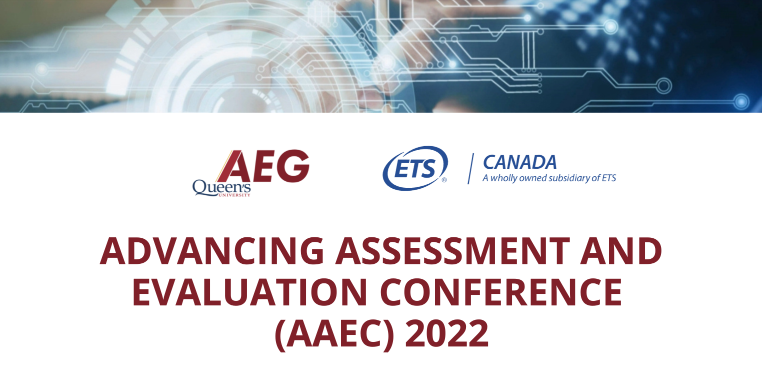
\includegraphics{Content/H.png}

\textbf{Description:} The science of language learning has advanced in recent years. This panel was devoted to thinking about how innovations in assessment and evaluation can provide further insights into language learning and assessment and to consider the application of these innovations in everyday practice.

The following questions were intended to inspire and generate ideas. The speakers did not need to address the questions directly.

\begin{itemize}
\item
  What new assessment and evaluation approaches can be used to promote language learning?
\item
  How is the role of assessment of language learning changing?
\item
  What are important considerations for language learning and assessment in our current context?
\item
  What variations in language learning strategies exist and how do these mirror assessment
  and evaluation practices?
\end{itemize}

\newpage

\hypertarget{an-ecosystem-symbiosis-among-learning-teaching-and-assessment}{%
\section{An Ecosystem: Symbiosis Among Learning, Teaching, and Assessment}\label{an-ecosystem-symbiosis-among-learning-teaching-and-assessment}}

\textbf{Author:} Liying Cheng, PhD

\textbf{Institution:} Queen's University

\textbf{Recommended Citation:}

\begin{quote}
Cheng, L. (2022, January 27-28). \emph{An Ecosystem: Symbiosis Among Learning, Teaching, and Assessment} {[}Paper presentation{]}. Advancing Assessment and Evaluation Virtual Conference: Queen's University Assessment and Evaluation Group (AEG) and Educational Testing Services (ETS), Kingston, Ontario, Canada.
\end{quote}

Let us imagine an ecosystem of language learning and learners where a symbiosis among elements of learning, teaching and assessment is achieved -- living, alive, and sustainable. Symbiosis is a biology term to describe ``the art of living together'' where the relationship or interaction among different or dissimilar organisms benefit from each other. In educational assessment, this relationship is referred to as washback and consequential validity where we explore the symbiotic relationship among learning, teaching and assessment in supporting our learners and their learning. And that is the research that I have been working on since my doctoral dissertation!

We now live in a very different world. The COVID-19 global pandemic, which we are still in the middle of, threatens our very survival and `thrival'. This pandemic has taught us hard lessons, and everything we thought we knew about our world and about our language learning has to be re-examined. We must reconceptualise learning, teaching and assessment (testing) individually, more importantly, together of the symbiotic relationships among the three. The current global travel restrictions (which for some countries may remain for a long time) require us to carefully consider the major changes in globalisation, internationalisation, and migration (transmigration) in relation to assessment (testing). Further, the geopolitics of assessment (Cheng, 2018, Volante, et. al., 2020) heightens the power of assessment (testing) in a given society, often leading to educational inequities and resentment toward assessment and testing.

All of these changes are happening at the same time as the exponential growth and development of artificial intelligence, natural language processing, and machine learning. We are facing vast opportunities and challenges to language learning, whether it is the first language learning, additional (second and foreign) language learning, bilingual and multilingual language learning in relation to teaching and assessment. The future of language learning and learners will redefine language constructs, assessment, and technology, challenge us to build an ecosystem where symbiosis could be achieved through a community or group of organic entities, within which all educational stakeholders -- humans and machines -- interact with each other in a symbiotic and mutually supportive environment.

I will illustrate this ecosystem using two potential areas of studies. The first project focuses on the system of learning (machine learning), teaching, and testing for supporting the language learning of international educated nurses. The second project turns to our young learners with whom we explore building their learning capacity in taking control, responsibility, and pride from an organic point of view bridging assessment and self-regulated learning.

\textbf{Building Canada's Healthcare One Nurse at a Time: An Ecological System for Testing, Learning, and Teaching}

The global COVID-19 pandemic changed our Canadian healthcare system, which has been stretched to its breaking point. Even before the pandemic, there was a serious shortage of registered nurses in Canada (Ariste et al., 2019); now, 1 in 3 Ontario nurses are considering leaving the profession due to the pandemic (CBC News, 2021). Hiring Internationally Educated Nurses (IENs) is essential to address this critical shortage (Boateng, 2015; Covell et al., 2017). However, IENs must pass a recertification test to be eligible to practice in Canada (Canadian Nurses Association, 2021), as well as demonstrate proficiency in English or French (e.g., British Columbia College of Nursing Professionals, 2019; College of Nurses of Ontario, 2020). Thus, while IENs have the potential to become key contributors to Canadian healthcare, they face multiple systemic barriers to recertification, with language posing a central challenge.

To continue our pandemic disrupted research on supporting IENs to accelerate their language proficiency for recertification, we propose to create an ecological system for testing, learning, and teaching as our innovative research methodologies. In this ecosystem, we challenge the conventional models where testing, learning, and teaching are conducted separately and where test developers and raters, IENs as test-takers, nursing bridging educators, language teachers, and researchers work in silos. We will build this system via an online supportive infrastructure so the collection of research data will be iterative, interactive, and symbiotic alongside testing, learning, and teaching data. Furthermore, this system can collect data from these stakeholders individually, within one group of the stakeholders, and from the interactions among all the stakeholders together, while at the same time this system is 100\% open-access and virtual worldwide. We aim to create the first of its kind integrated teaching, learning, and testing ecosystem housed in Canada, serving IENs and many other internationally educated professionals (IEPs) for a stronger Canadian immigration mosaic across all professions and industries, including healthcare.

\textbf{Learning to Love Learning: Taking Control, Responsibility, and Pride through Self-Regulated Learning and Assessment}

The worldwide impact of the COVID-19 pandemic on education has been largely impossible to imagine, predict, and measure. As a result, traditional modes and methods of learning and assessment have been challenged, and the quality of our education systems has been questioned -- on a global scale. This unprecedented disruption to education has had a tremendous negative impact on the learning of all students, particularly our young elementary school students who are most vulnerable (Timmons et al., 2021). At the same time, their parents are being put to a strenuous test, juggling their work duties with their parenting responsibilities -- all in a full-time capacity. These global challenges faced by parents and children have highlighted and magnified the importance of students becoming self-regulated learners. A self-regulated learner has the capacity to monitor their own learning, set goals for themselves, establish plans and access resources to achieve their goals, and assess their own progress. Self-regulated learning (SRL), a fundamental goal of our education systems, ultimately allows a student to take control, responsibility, and pride in their learning -- driving their learning forward, not only during schooling but throughout their entire lives. Importantly, this ability of students, and all citizens, to self-regulate has been one of the central indicators for success during the global COVID-19 pandemic (Pelikan et al., 2021; Santamaría-Vázquez et al., 2021). However, the global pandemic has elucidated the diversity of socio-cultural values embedded in learning and assessment across educational systems internationally, including how SRL is endorsed and supported. The proposed study serves to promote this essential education goal of SRL by leveraging prior literature that predicts classroom assessment practices as a powerful approach to promote the development of SRL in young learners (DeLuca et al., 2020). The overall goal is to examine how SRL as a quality assessment strategy can support elementary students in Canada and China to take control, responsibility, and pride in their learning.

\textbf{References}

Ariste, R., Béjaoui, A., \& Dauphin, A. (2019). Critical analysis of nurses' labour market effectiveness in Canada: The hidden aspects of the shortage. The International Journal of Health Planning and Management, 34(4), 1144-1154. \url{https://doi.org/10.1002/hpm.2772}

Boateng, G. O. (2015). Exploring the career pathways, professional integration, and lived experiences of regulated nurses in Ontario, Canada {[}Unpublished doctoral dissertation{]}. The University of Western Ontario.

British Columbia College of Nursing Professionals. (2019). English requirements. Internationally Educated Nurses. \url{https://www.bccnp.ca/Registration/RN_NP/RNApplication/InternationalEN/Pages/Englishrequirements.aspx}

Canadian Nurses Association. (2021). Work in Canada. Retrieved October 8, 2021, \url{https://www.cna-aiic.ca/en/nursing-practice/career-development/work-in-canada}

CBC News. (2021). 1 in 3 Ontario registered practical nurses considering quitting due to pandemic, poll suggests. Retrieved August 22, 2021, \url{https://www.cbc.ca/news/canada/toronto/nurses-ontario-covid-19-burnout-survey-1.5890799}

Cheng. L. (2018). Geopolitics of assessment. In S. Abrar-ul-Hassan (Ed.), TESOL encyclopedia of English language teaching: Teaching English as an international language. Hoboken, NJ: John Wiley \& Sons. \url{https://doi.org/10.1002/9781118784235.eelt0814}

College of Nurses of Ontario. (2020). In-depth: Language proficiency. Registration Requirements. \url{https://www.cno.org/en/become-a-nurse/registration-requirements/language-proficiency/in-depth-language-proficiency/}

Covell, C. L., Primeau, M. D., Kilpatrick, K., \& St-Pierre, I. (2017). Internationally educated nurses in Canada: Predictors of workforce integration. Human Resources for Health, 15(1), 1-16. \url{https://doi.org/10.1186/s12960-017-0201-8}

DeLuca, C., Pyle, A., Braund, H., \& Faith, L. (2020). Leveraging assessment to promote kindergarten learners' independence and self-regulation within play-based classrooms. Assessment in Education: Principles, Policy \& Practice, 27(4), 394-415. \url{doi:10.1080/0969594X.2020.1719033}

Pelikan, E.R., Lüftenegger, M., Holzer, J. et al.~(2021). Learning during COVID-19: The role of self-regulated learning, motivation, and procrastination for perceived competence. Z Erziehungswiss, 24, 393--418. \url{https://doi.org/10.1007/s11618-021-01002-x}

Santamaría-Vázquez, M.; Del Líbano, M.; Martínez-Lezaun, I.; Ortiz-Huerta, J.H. Self-Regulation of motivation and confinement by COVID-19: A study in Spanish university students. (2021). Sustainability, 13, 5435. \url{https://doi.org/} 10.3390/su13105435

Timmons, K., Cooper, A., Bozek, E., \& Braund, H. (2021). The impacts of COVID-19 on early childhood education: Capturing the unique challenges associated with remote teaching and learning in K-2. Early Childhood Educational Journal, 49, 887-901. \url{https://doi.org/10.1007/s10643-021-01207-z}

Volante, L., DeLuca, C., Adie, L., Baker, E., Harju‐Luukkainen, H., Heritage, M., Schneider, C., Stobart, G., Tan, K. and Wyatt‐Smith, C. (2020), Synergy and Tension between Large‐Scale and Classroom Assessment: International Trends. Educational Measurement: Issues and Practice, 39: 21-29.

\newpage

\hypertarget{ai-assisted-spoken-language-learning-for-mobile-and-computer-applications}{%
\section{AI Assisted Spoken Language Learning for mobile and computer applications}\label{ai-assisted-spoken-language-learning-for-mobile-and-computer-applications}}

\textbf{Author:} Rutuja Ubale

\textbf{Organization:} Educational Testing Service (ETS)

\textbf{Recommended Citation:}

\begin{quote}
Ubale, R. (2022, January 27-28). \emph{AI Assisted Spoken Language Learning for mobile and computer applications} {[}Paper presentation{]}. Advancing Assessment and Evaluation Virtual Conference: Queen's University Assessment and Evaluation Group (AEG) and Educational Testing Services (ETS), Kingston, Ontario, Canada.
\end{quote}

The COVID-19 pandemic has impacted every aspect of our lives. This includes requiring students to engage in remote learning from home, a need that we were perhaps not very well prepared for in the pre-pandemic times in terms of technology which had suddenly become a necessity. Teachers have been trying to invent ways of bringing more engaging instruction, create targeted practice and evaluate student homework. Several E-learning and language learning platforms like Duolingo, Busuu, ELSA Speak, etc. saw tremendous increase in the number of users over the last year.

AI-powered apps can provide personalized feedback and learning by recognizing learner's strengths and weaknesses using machine learning algorithms on written and spoken responses. However, students can be impeded by negative feedback which is not constructive enough to be useful to inform their learning journey.

\textbf{Challenges in Language Learning:}

\begin{enumerate}
\def\labelenumi{\arabic{enumi}.}
\tightlist
\item
  Lack of motivation
\end{enumerate}

Lessons can be too repetitive and teachers often feel challenged to create new interesting practice material. Learners can get bored of repetitive content in learning apps and begin disengaging leading to poor user retention rates. The main reasons for it are too long lessons, boring exercises, unfitting difficulty level, insufficient rules explanation, or absence of personalization. Using AI and natural language processing technology can enable automatic generation of a diversity of exercise types to alter different types of activities and avoid boredom. Placement test can be used to detect the current level and start learning from that point. Creation of customized and adaptive learning paths to offer only relevant materials to master based on the learner's skill acquisition can enable better user engagement and learning experience. Gamified environments that include goal-setting like achievement badge, daily streaks, a level, a position on a leaderboard, opportunities for social interaction and competition with adaptive leaderboards as per studies {[}1{]} lead to stronger motivation and increased performance.

\begin{enumerate}
\def\labelenumi{\arabic{enumi}.}
\setcounter{enumi}{1}
\tightlist
\item
  Knowledge Retention
\end{enumerate}

In app based learning, newly learned information can be easily forgotten with continuous repeated practice as users continue to see newer practice material and concepts. It has been observed in research that data-driven spaced repetition to repeat new information over short intervals of time leads to better knowledge retention as opposed to massed practice or cramming. The spaced repetition technique has been adopted by several language learning apps including Duolingo {[}3{]} that reportedly saw an increase in learner engagement by 12\% in an operational user study. Regular AI based automated assessments and continuous feedback to detect learners' knowledge gaps and customized learning path with the concepts to practice and master can also help improve knowledge acquisition and retention.

\begin{enumerate}
\def\labelenumi{\arabic{enumi}.}
\setcounter{enumi}{2}
\tightlist
\item
  Overcoming language barriers
\end{enumerate}

Many learners don't have access to real life scenarios while mastering a language for example native speakers of a language that they can speak with to practice real-life conversations and improve their confidence speaking in the language being learnt. Speech recognition can help learners to engage in speaking, even without a partner being available. AI can be used to simulate real-life conversational practice with chatbots using speech recognition, natural language understanding as well as immersive learning experience with augmented reality and virtual reality technology. Social networking in app to allow interaction with fellow learners, peers or native speakers can also provide real-life usage scenarios.

\begin{enumerate}
\def\labelenumi{\arabic{enumi}.}
\setcounter{enumi}{3}
\tightlist
\item
  Targeted and actionable feedback
\end{enumerate}

In second language (L2) learning solutions, intuitive learning is good at the beginning when concepts and exercises are simple. ASR based language learning solutions can provide instant feedback on the student's speaking performance. But once the exercises become more complex, learners need deeper feedback and explanations for their mistakes. Without such support a learner will always repeat the same mistakes and be confused on how to move forward with their learning. Here's a quote from the review from LearnJam on the Speaking Pal, a spoken language learning platform `The `feedback' consisted of showing me which words I'd said `well' (in green) and which ones I needed to work on (red). There doesn't seem to be an explanation as to what in particular the problem is with my speaking, so I'm none the wiser as to how to improve. I just tried to shout it a couple of times to be sure' {[}4{]}. One solution is scaffolded support to give on-demand explanation during exercises or in case of mistakes.

\textbf{Technologies used in spoken language learning and teaching}

\emph{Automatic Speech Recognition:}

Use of automatic speech recognition allows the learners to converse with computer/ mobile phone. ASR turns speech into written text by using a speech recognition engine. Speech recognition engines are software systems that take users' speech as audio input (i.e.~digital
audio signals from a microphone or recording) and process the stream of sound into individual sounds, vowels and consonants, lexical items and outputs a transcription of the user's speech. This transcription can then be presented to user as an indication of what the user said or be used as input to speech and natural language processing systems to extract deeper evaluation of the user's speech to provide feedback on grammar and content. Speech recognition systems can be used to also measure the speed at which the learners speak, and rate of speech has been shown to correlate with speaker proficiency.

\emph{Pronunciation Error Detection:}

One worthy area of focus of speech technology is pronunciation. Voice-interactive pronunciation tutors can prompt students to repeat spoken words and phrases or to read aloud sentences in the target language for the purpose of practicing both the sounds and the intonation of the language. The key to teaching pronunciation successfully is corrective feedback, more specifically, a type of feedback that does not rely on the student's own perception. Automatic pronunciation scoring can serve as a means to evaluate spoken learner productions in terms of fluency, segmental quality (phonemes) and supra-segmental features (intonation). The automatically generated proficiency score can then be used as a basis for providing other modes of corrective feedback. These systems can be built by evaluating the quality of the user's speech by first of all extracting information from audio signals that are supplied in machine learning or deep learning models to identify how close the user's production was to that of a native speaker, whether there is L1 interference (where the L1 is known) and whether L2 phones or specific production patterns are missing from the speech.

\emph{Speech synthesis:}

While computers can listen to, understand and use what we are saying, at least to a certain extent they can also be used to reply to users with feedback or to teach the users specific usage or pronunciation. This is done using speech synthesis software otherwise known as text-to-speech (TTS) engines. This uses the basic audio features of a computer to create spoken audio output from written text. While the goal of TTS systems is mimic human speech, most state-of-the-art TTS systems to date still sound a bit artificial and a lot of most recent research has been targeted at generating more natural and emotional speech synthesis.

\emph{Automated assessment and feedback engines:}

Evaluating students' speech output, generating tests and assignments and giving individual feedback is one of the most time-consuming tasks that a teacher can face. Speech technology can be used to automate the evaluation of learner's spoken production. Learner's speech can be fed through the same speech recognition and analysis systems followed by a machine or deep learning based scoring and feedback model to display actionable insights to users. The speech is analyzed both in terms of its content (i.e.~what is in the transcribed text) and its pronunciation and prosody features (i.e.~what it sounds like in the audio version of the speech).

\textbf{Summary}

We've looked at the different challenges in building efficient and effective language learning applications using AI and what features popular language learning apps have developed to improve user engagement. Additionally, we also discuss different speech technologies that are leveraged in spoken language learning solutions to assess, evaluate and generate targeted feedback for learners to help them advance in their learning journey.

\textbf{References:}

\begin{enumerate}
\def\labelenumi{\arabic{enumi}.}
\item
  The Effect of Achievement Badges on Students' Behavior: An Empirical Study in a University-Level Computer Science Course
\item
  H. Ebbinghaus. 1885. Memory: A Contribution to Experimental Psychology. Teachers College,
  Columbia University, New York, NY, USA.
\item
  Settles, B. and Meeder, B., 2016, August. A trainable spaced repetition model for language learning. In Proceedings of the 54th annual meeting of the association for computational linguistics (volume 1: long papers) (pp.~1848-1858).
\item
  Gifford, T. (2013, November). Speech Recognition apps for ELT: SpeakingPal English tutor. ELTjam. Retrieved from \url{https://eltjam.com/speechrecognition-apps-for-elt-speakingpal-englishtutor}
\end{enumerate}

\newpage

\hypertarget{the-power-of-diagnostic-scaffolding-in-technology-rich-learning-oriented-assessment-environments}{%
\section{The Power of Diagnostic Scaffolding in Technology-Rich Learning-Oriented Assessment Environments}\label{the-power-of-diagnostic-scaffolding-in-technology-rich-learning-oriented-assessment-environments}}

\textbf{Author:} Eunice Eunhee Jang, PhD

\textbf{Institution:} University of Toronto

\textbf{Recommended Citation:}

\begin{quote}
Jang, E. E. (2022, January 27-28). \emph{The Power of Diagnostic Scaffolding in Technology-Rich Learning-Oriented Assessment Environments} {[}Paper presentation{]}. Advancing Assessment and Evaluation Virtual Conference: Queen's University Assessment and Evaluation Group (AEG) and Educational Testing Services (ETS), Kingston, Ontario, Canada.
\end{quote}

Since the introduction of DIALANG (Alderson \& Huhta, 2005), technological advances have made possible timely, dynamic, and multi-agent delivery of assessment results and feedback for learners. In particular, new horizons have opened with performative task designs. They are infused with authentic audio and video stimuli (Wagner, 2008), spontaneous performance modes, adaptive scaffolding (Azevedo, Cromley, \& Seibert, 2004; Deville \& Chalhoub-Deville, 1999), and simultaneous assessment of integrative skills through multidimensional mastery skill profiling (Jang, 2005; Leighton \& Gierl, 2007; Yan, Almond, \& Mislevy, 2004).

Afforded by rapid advances in technological innovations, natural language processing and machine learning are increasingly used to recognize, interpret, and generate human languages in productive skills, such as oral (Evanini, Heilman, Wang, \& Blanchard, 2015; Zechner, Higgins, Xi, \& Williamson, 2009) and written abilities (Burstein, Chodorow, \& Leacock, 2004; Crossley, Kyle, \& McNamara, 2016). Real-time data processing allows for timely and adaptive feedback for students, which can be used for expert, interactive, and self-scaffolding during task performance (Xi, 2010). Automated feedback systems can transform learning-oriented assessment by integrating instantaneous performance feedback into the context of real-time learning.

Argument-based validity theories offer guiding principles for evaluating automated scoring and feedback systems (Chapelle \& Chung, 2010; Kane, 2013). While evaluation, generalization, and explanation inferences are central to the validity argument for large-scale standardized testing programs, utilization inferences are especially critical for teaching and learning. Interpretive arguments concerning the utilization inference typically seek evidence to support the claim that automated feedback positively impacts student learning.

Previous research on feedback has focused chiefly on the impact of feedback formats (Ellis, Loewen, \& Erlam, 2006; Ferris, 2010). Little research other than research on dynamic assessment (Lantolf \& Poehner, 2004; Leung, 2007) has addressed its scaffolding mechanisms in assessing productive skills in technology-rich environments. Mediation through feedback during task performance can be distinct from end-of-task feedback as it provides simultaneous diagnosis and scaffolding (Lantolf \& Poehner, 2008). It differs further by an agency (Holton \& Clarke, 2006). While the mediator leads expert scaffolding to promote conceptual learning or skill development, reciprocal scaffolding can occur collaboratively through peer-to-peer or human-machine interactions. In addition, self-scaffolding can take place through learners' metacognitive control.

In this talk, I examine the mechanisms of scaffolding based on automated diagnostic feedback in BalanceAI, a technology-rich learning and assessment platform. It leverages automated scoring to provide real-time diagnostic feedback for teachers and students in four core areas: students' psychoeducational beliefs, literacy (writing and reading comprehension), oral language, and cognitive reasoning. The component of psychoeducational beliefs includes student self-assessment of self-efficacy, goal orientation, self-regulation, and grit. The literacy component includes a series of reading and writing activities. Five reading testlets include reading passages of which readability varies from Grades 2 to 8 and engage students in innovative tasks beyond typical reading comprehension questions. Students and teachers receive skill mastery profiles on their respective dashboards. The writing component engages students in a series of writing activities, including watching video stimuli, prewriting, drafting an essay, revising it, and self-assessment of writing skills after submitting the revised essay. Students' essays are automatically scored over five analytic criteria. Teachers have an option to evaluate their students' essays as well. The writing dashboard provides automated essay scores alongside teachers' assessments. The third component of BalanceAI includes six different oral and cognitive reasoning tasks. Students' reading fluency is automatically scored based on their read- aloud. Oral language proficiency is automatically scored based on picture description and story- retell tasks. Phonological awareness is assessed using elision tasks. Two cognitive reasoning tasks assess students' short-term memory capacity and fluid reasoning ability.

The BalanceAI assessment system has been used by various teachers, educators, and students in different contexts---the first field research involved over 200 students in elementary schools. Over 500 students have used it in classrooms for the past two years. For the past year, community outreach programs have used it as a digital support tool for students from urban shelters, refugees, language learners, and other students with limited learning opportunities due to school closure during the pandemic.

Individual students completed 8-10 one-to-one sessions in the community outreach program. Tutors received extensive training on the theoretical grounds of target constructs, interpretation of real-time performance results, and diagnostic scaffolding before, during and after task performance. Some of the diagnostic scaffolding activities included verbalizing thoughts, setting goals, identifying own errors, and practicing skills identified through goal- setting.

In seeking validity evidence to support the effect of diagnostic scaffolding in the community outreach program, aggregating results across individuals deem problematic because of questionable assumptions about data properties and contextual variations. Dynamic complexity theory offers an alternative perspective for understanding a feedback mechanism as its cause and effect are often nuanced and complex (Larsen-Freeman, 2011; Wolf-Branigin, 2013). I examine three central characteristics of dynamic complexity theory applied to the BalanceAI learning context. They include self-organizing agency, co-adaptation, and sensitivity of initial conditions.

\textbf{Self-organizing agency}

In general, living agents, including human beings, self-organize their systems (Mainzer, 2007). How do self-organizing learners look? Self-organized learning involves:

\begin{itemize}
\item
  Initiating and organizing own learning.
\item
  Aligning individual learning with larger goals.
\item
  Being self-aware of their strengths and weaknesses.
\item
  Seeking feedback.
\item
  Regulating behaviours.
\item
  Adapting to changing environments.
\end{itemize}

This iterative self-organizing process is called `soft-assembly' (Larsen-Freeman, 2011; Thelen \& Smith, 1994). As learners engage with learning-oriented tasks and receive real-time feedback, they constantly consider options and constraints and assemble resources dynamically.

\textbf{Co-adaptation}

The BalanceAI learning-oriented digital assessment platform is intended to redesign the
relationship between learning and assessment and facilitate dynamical co-adaptions between agents. As learners interact with their teacher or tutor, their cognitive, affective, and metacognitive resources are altered, the agents experience `coupling of complex systems' (Thelen \& Smith, 1994). Actions taken as a response to various task features lead to emerging patterns in learning. This iterative co-adaptation process prompts the emergence of stable patterns from local learning.

\textbf{The edge of chaos}

Students' initial conditions matter significantly. Change in learning occurs gradually in nonlinear patterns. Changes are not necessarily proportionally subject to the dosage of causes due to their sensitivity to initial conditions. Complex systems are chaotic and dynamical as they are susceptible to initial conditions. That sensitivity is known as a butterfly effect, referring to small changes over time in the initial state that leads to a more significant and unpredictable impact (Lorenz, 1963). For example, a learner who struggles with writing experiences assistive technology that translates her speech to text first. The surprise that the learner experiences with the assistive technology may lead to dramatic changes in her cognitive growth.

In closing, automated feedback systems provide an opportunity to create a dynamic learning system in which learners develop self-organizing principles, assemble resources, and adapt to their own and external contexts. Individual differences in initial conditions play a critical role as nonlinear patterns emerge dynamically. Automated diagnostic feedback systems provide critical real-time input for co-adaptive interactions among agents.

\textbf{References}

Alders-on, J. C., \& Huhta, A. (2005). The development of a suite of computer-based diagnostic tests based on the Common European Framework. Language Testing, 22(3), 301-320.

Azevedo, R., Cromley, J. G., \& Seibert, D. (2004). Does adaptive scaffolding facilitate students' ability to regulate their learning with hypermedia?. Contemporary Educational Psychology, 29(3), 344-370.

Burstein, J., Chodorow, M., \& Leacock, C. (2004). Automated essay evaluation: The Criterion online writing service. Ai Magazine, 25(3), 27-27.

Chalhoub--Deville, M., \& Deville, C. (1999). Computer adaptive testing in second language contexts. Annual Review of Applied Linguistics, 19, 273-299.

Chapelle, C. A., \& Chung, Y. R. (2010). The promise of NLP and speech processing technologies in language assessment. Language Testing, 27(3), 301-315.

Crossley, S. A., Kyle, K., \& McNamara, D. S. (2016). The tool for the automatic analysis of text cohesion (TAACO): Automatic assessment of local, global, and text cohesion. Behavior Research Methods, 48(4), 1227-1237.

Ellis, R., Loewen, S., \& Erlam, R. (2006). Implicit and explicit corrective feedback and the acquisition of L2 grammar. Studies in Second Language Acquisition, 28(2), 339-368.

Evanini, K., Heilman, M., Wang, X., \& Blanchard, D. (2015). Automated scoring for the TOEFL Junior® Comprehensive writing and speaking test. ETS Research Report Series, 2015(1), 1-11.

Ferris, D. R. (2010). Second language writing research and written corrective feedback in SLA: Intersections and practical applications. Studies in Second Language Acquisition, 32(2), 181-201.

Holton, D.A., \& Clarke, D. (2006). Scaffolding and metacognition. International Journal of Mathematical Education in Science and Technology, 37, 127-143.

Jang, E. E. (2005). A validity narrative: Effects of reading skills diagnosis on teaching and learning in the context of NG TOEFL. University of Illinois at Urbana-Champaign.

Kane, M. (2013). The argument-based approach to validation. School Psychology Review, 42(4), 448-457.

Larsen-Freeman, D. (2011). A complexity theory approach to second language development/acquisition. In Atkinson, D. (Ed.), Alternative approaches to second language acquisition (pp.~60-84). Routledge.

Leighton, J., \& Gierl, M. (Eds.). (2007). Cognitive diagnostic assessment for education: Theory and applications. Cambridge University Press.

Leung, C. (2007). Dynamic assessment: Assessment for and as teaching?. Language Assessment Quarterly, 4(3), 257-278.

Lorenz, E. N. (1963). Deterministic nonperiodic flow. Journal of the Atmospheric Sciences, 20(2), 130-141.

Mainzer, K. (2007). Thinking in complexity: The computational dynamics of matter, mind, and mankind. Springer Science \& Business Media.

Poehner, M. E., \& Lantolf, J. P. (2005). Dynamic assessment in the language classroom. Language Teaching Research, 9(3), 233-265.

Thelen, E., \& Smith, L. B. (1994). A dynamic systems approach to the development of cognition and action. The MIT Press.

Wagner, E. (2008). Video listening tests: What are they measuring?. Language Assessment Quarterly, 5(3), 218-243.

Wolf-Branigin, M. (2013). Using complexity theory for research and program evaluation. Oxford University Press.

Xi, X. (2010). Automated scoring and feedback systems: Where are we and where are we heading?. Language Testing, 27(3), 291-300.

Yan, D., Almond, R., \& Mislevy, R. (2004). A comparison of two models for cognitive diagnosis. ETS Research Report Series, 2004(1), i-33.

Zechner, K., Higgins, D., Xi, X., \& Williamson, D. M. (2009). Automatic scoring of non-native spontaneous speech in tests of spoken English. Speech Communication, 51(10), 883-895.

\newpage

\hypertarget{reflections-on-incorporating-an-anti-racist-pedagogy-into-a-language-testing-and-assessment-course-a-critical-need-for-more-research}{%
\section{Reflections on incorporating an anti-racist pedagogy into a language testing and assessment course: A critical need for more research}\label{reflections-on-incorporating-an-anti-racist-pedagogy-into-a-language-testing-and-assessment-course-a-critical-need-for-more-research}}

\textbf{Author:} Christine Doe, PhD

\textbf{Institution:} Mount Saint Vincent University

\textbf{Recommended Citation:}

\begin{quote}
Doe, C. (2022, January 27-28). \emph{Reflections on incorporating an anti-racist pedagogy into a language testing and assessment course: A critical need for more research} {[}Paper presentation{]}. Advancing Assessment and Evaluation Virtual Conference: Queen's University Assessment and Evaluation Group (AEG) and Educational Testing Services (ETS), Kingston, Ontario, Canada.
\end{quote}

This presentation considers my experience of incorporating an anti-racist pedagogy into a language testing course for the Fall of 2021. I am presenting this topic to respond to how the field of assessment and evaluation can better promote language learning. The reason for this is two-fold. First, like any research field, language testing and assessment must respond to the call of taking a critical stance on racism (Kubota, 2019). Second, teachers need to facilitate and promote language learning opportunities based on culturally responsive and appropriate assessments (Esch, Motha \& Kubota, 2020). Thus, through classroom language assessment training from an anti-racist pedagogy, pre-service and in-service teachers can adequately meet the needs of their students in using appropriate language assessment practices.

There is a need for critical pedagogies that dismantle the systematic racism entrenched throughout all levels of education (e.g., Kishimoto, 2018; Mayorga \& Picower, 2017; Reddington, Theunissen \& MeDrano, 2021). As someone teaching in education, the use of critical pedagogical lens is becoming more mainstream. To adequately prepare pre-service teachers, I needed to incorporate anti-racism education into my teaching and model it (Mayorga \& Picower, 2017). Promoting and fighting for equity is no longer on the fringes or the sole responsibility of BIPOC and other equity-seeking groups or subjects focused on social justice and equity. Thus, it was essential to incorporate an anti-racist pedagogy into my preparation and teaching of the Fall 2021 Language Testing and Assessment course. Anti-racist pedagogy in a higher education setting, as defined by Kishimoto (2018), includes three components of (1) integrating the topics of race and inequality throughout the course, (2) ensuring that the `how' of teaching comes from an anti-racist pedagogy, and (3) doing activities beyond the classroom to promote anti-racist efforts throughout the campus.

For the purposes of this presentation, I aim to do two things. First, to share my preliminary findings of searching the language testing literature for the topics of race and inequality (i.e., component one of the anti-racist pedagogy). And second, to comment on some strategies for incorporating an anti-racist pedagogy into a language testing course (i.e., component two of the anti-racist pedagogy). In my initial search for resources in the summer of 2021, I looked to the key handbooks on language testing, such as the 2021 Handbook of Second Language Acquisition and Language Testing by Paula Winke and Tineke Brunfaut and searches through key databases like the Linguistics and Language Behavior Abstracts (LLBA). I was surprised to find limited resources on the topic, which inspired the topic for this presentation. To prepare for this presentation, I employed a more systematic search strategy to identify literature from an anti-racist framework.

I searched three key sources of research on language testing and assessment: (1) the 1999-2020 ILTA bibliography, (2) the LLBA database, and (3) Education Research Complete (EBSCO). I selected six broad search categories: racism (variations: race and racist); social justice (variations: justice, equity, critical language testing), Critical Race Theory, anti-racist frameworks (variations: anti-racist pedagogy/education, anti-Black racism, anti-Asian racism, and anti-Indigenous racism); multilingual (variations: bilingual, translanguaging), and multiculturalism (variations: intercultural, diversity/diverse). For every search in the two databases of LLBA and Education Research Complete, the Boolean phrase (``language testing'' or ``language assessment'') was used in combination with each term for the six search categories in the abstract or title field. My search parameters also included the dates of 1991 to 2022 to capture 20 years of publication history. Since the analysis was conducted in January of 2022, I did not count 2022 as a publication year, but I did include it to be as exhaustive as possible. I then did a third round of searching in LLBA to look for the search categories specifically in language testing and assessment journals. To do this, I used the terms ``language testing'' and ``language assessment'' for publication title to capture the research articles from two key journals of the field: Language Testing and Language Assessment Quarterly. With each search result, I reviewed the titles and abstracts to make sure they fit with the categories considered. For the interest of time, when the search results had 20 or less I was able to see if there were any duplications. However, I was not able to do the same when the counts were higher. Thus, it is important to recognize that the search and analysis I conducted did not have the rigour of a systematic review (Macaro, 2019). Nevertheless, I do believe there can be some broad observations made from the preliminary findings.

Similar to my findings this past summer, I found no resources that related to research from a Critical Race Theory (Dixson \& Rousseau, 2016) perspective or any form of anti-racist pedagogy/education framework. Within the search category of race, I was able to find four articles and one PhD Dissertation that considered the topic of race as it related to inequity (Blackledge, 2006; Fleming, 2016; Hammond, 2019; McNamara, 2009; Milani, 2008; Sterzuk, 2007). Only one of the resources (McNamara, 2009) was from a language testing journal. It is concerning that there were so few research resources with the topic of race and racism, which was in contrast to the over 20 articles on the topics of social justice, equity and fairness. Interestingly, it was most productive to search for social justice and equity category within the journals that had language testing or language assessment in the title: social justice (5), justice (12), equity (7), critical language testing (3). The number of articles identified under the social justice category is not surprising considering the more than 15 years where there has been a push and call for the social dimension of language testing (McNamara \& Roever, 2006). It should be noted that for the search of the literature, I only included the search terms for the title and abstract, and for the ILTA bibliography it was only the title. If I had conducted the searches with the terms in the full text field, I would have identified more articles. For instance, the search for the race category did not identify the introduction by Schissel and Khan (2021) for the virtual special issue in the journal Language Testing, because the introduction did not include an abstract or have race in the title. However, Schissel and Khan do provide a thought-provoking commentary on the state of the field of language testing and the need to consider language testing research from anti-oppressive frameworks.

Overall, these preliminary findings highlight how the field needs to expand language testing research and test use to include anti-oppressive research theories, such as Critical Race Theory (Dixson \& Rousseau, 2016). Further, the field needs to examine and expand the discussions on how to employ anti-racist pedagogies into language testing training.
This presentation will report on my initial searches of looking for research and resources, the observations made from my search, and the implications for teaching a language testing and assessment course from an anti-racist pedagogy. To conclude the presentation, I will pose some questions to the audience to gain their thoughts and comments about how to address the gaps in the literature.

\textbf{References}

Blackledge, A. (2006). The racialization of language in British political discourse. Critical Discourse Studies, 3(1), 61-79.

Dixson, A. D., \& Rousseau, C. K. (2016). Critical race theory in education: All god's children got a song. New York: Routledge.

Fleming, D. (2015). Citizenship and race in second-language education. Journal of Multilingual and Multicultural Development, 36(1), 42-52.

Hammond, J. W. (2019). Making our invisible racial agendas visible: Race talk in Assessing Writing, 1994--2018. Special Issue: Framing the Future of Writing Assessment, 42, 100425. \url{https://doi.org/10.1016/j.asw.2019.100425}

Kishimoto, K. (2018) Anti-racist pedagogy: from faculty's self-reflection to organizing within and beyond the classroom. Race Ethnicity and Education, 21(4), 540-554. doi: 10.1080/13613324.2016.1248824

Kubota, R. (2019). Confronting epistemological racism, decolonizing scholarly knowledge: Race and gender in applied linguistics. Applied Linguistics, 41(5), 1--22.

Macaro, E. (2019). Systematic reviews in applied linguistics. In Ed. Jim McKinley and Heath Rose, The Routledge Handbook of Research Methods in Applied Linguistics (pp.~230-239). Routledge.

Mayorga E., \& Picower B. (2018) Active Solidarity: Centering the Demands and Vision of the Black Lives Matter Movement in Teacher Education. Urban Education, 53(2), 212-230. \url{doi:10.1177/0042085917747117}

McNamara, T. (2009). Australia: The dictation test redux? Language Assessment Quarterly, 6(1), 106. \url{doi:http://dx.doi.org/10.1080/15434300802606663}

Reddington, S., Theunissen, S., \& MeDrano, J. (2021). Conditions for Success: Indigenous Youth Reflections on Their Experiences with Canadian Education Systems. INYI Journal, 11(1), 1-10. \url{https://doi.org/10.25071/1929-8471.73}

Schissel, J. L., \& Khan, K. (2021). Responsibilities and opportunities in language testing with respect to historicized forms of socio-political discrimination: A matter of academic citizenship. Language Testing, 38(4), 640--648.

Sterzuk, A. (2008). Dialect speakers, academic achievement, and power: First nations and Metis children in standard English classrooms in Saskatchewan {[}Unpublished doctoral dissertation{]}. McGill University.

Von Esch, K. S., Motha, S., \& Kubota, R. (2020). Race and language teaching. Language Teaching, 53(4), 391-421.

Winke, P., \& Brunfaut, T. (Eds.). (2020). The Routledge Handbook of Second Language Acquisition and Language Testing. Routledge.

\newpage

\hypertarget{feeding-forward-from-black-boxes-challenges-to-ensuring-just-educational-measurement-of-language-proficiency-in-an-age-of-automated-scoring-machine-learning-and-artificial-intelligence}{%
\section{``Feeding forward'' from ``black boxes''? Challenges to ensuring just educational measurement of language proficiency in an age of automated scoring, machine learning and artificial intelligence}\label{feeding-forward-from-black-boxes-challenges-to-ensuring-just-educational-measurement-of-language-proficiency-in-an-age-of-automated-scoring-machine-learning-and-artificial-intelligence}}

\textbf{Author:} Gregory Tweedie, PhD

\textbf{Institution:} University of Calgary

\textbf{Recommended Citation:}

\begin{quote}
Tweedie, G. (2022, January 27-28). \emph{``Feeding forward'' from ``black boxes''? Challenges to ensuring just educational measurement of language proficiency in an age of automated scoring, machine learning and artificial intelligence} {[}Paper presentation{]}. Advancing Assessment and Evaluation Virtual Conference: Queen's University Assessment and Evaluation Group (AEG) and Educational Testing Services (ETS), Kingston, Ontario, Canada.
\end{quote}

Many, if not most educators affirm, at least in theory, the notion of assessment for learning; namely that assessment should be used to provide information to teachers and students which will enable both parties to modify, to fruitful effect, the teaching and learning activities in which they are engaged. Some educators have cleverly referred to this process as feed-forward as opposed to feedback (e.g., Orsmund and colleagues, 2011), meaning that teacher feedback on student work is given in such a way that it can be utilised by students to inform and improve future assignments.

And yet, we observe as language educators two ubiquitous phenomena that would seem to create conditions standing in stark contrast to the notion of assessment for learning: high stakes testing, and automated scoring. High stakes language testing, if proprietary and commercially driven, typically thrives in a one-off model: test takers are assessed, and provided a score, but given no feedback on their performance to improve next time. In a commercial environment this is of course logical: the testing organisation benefits from repeat test-takers, and has little incentive, other than public image, to reduce the number of times individuals sit their test. Feedback to improve test-taker performance, in a strictly profit-driven setting, would be bad for business.

A second phenomena which may create conditions in opposition to assessment for learning is automated scoring (AS), particularly AS that draws upon machine learning models. Machine learning for automated scoring, when using a method known as massive deep learning models, draws from open-source corpora of billions of words, with billions of parameters, and then deploys increasingly complex statistical models to compare a test-taker's performance to that of the corpora. We end up with a score for the test-taker, but how we arrived at it is, for all intents and purposes, unexplainable. In fact, machine learning and its deep neural networks are often critiqued as ``black boxes'', and computer scientists often speak of the ``black box problem'' (e.g., Pardo et al, 2019), wherein we are unable to tell which aspects of a neural network are solving which computing task. Neural networks are a type of artificial intelligence modelled on the human brain, and are thought to be much better than standard algorithms at solving real-world problems. But unfortunately, as one researcher put it, neural networks are ``also as opaque as the brain'' (Castelvecchi, 2016, p.~2021). Instead of storing the information neatly, as we might in a database, machine learning diffuses it. Just like in the brain, information in a neural net is stored among its connections, not in a specific location. Machine learning with massive deep learning models can tell us what it concludes, but only opaquely how it arrived there.

So imagine a situation where testing organisations offer a high stakes, profit-driven form of language testing, while using opaque automated scoring from deep neural networks. This combination, by the way, is expected to be increasingly common in a post-pandemic environment: a perfect storm in which assessment for learning seems but a distant memory.

\emph{\textsuperscript{1} It is important to point out that machine learning is also used for providing formative feedback to learners (see, for example, WriteToLearn™ ¨{[}Pearson Assessments, 2022{]}), and that some testing organisations provide pre-test feedback to test candidates (see, for example IELTS Partners, 2022).}

We contrast zero-feedback language testing, administered via black box deep neural network models, with the framework of just educational measurement, as put forth by Zachary Stein (2016). In the book Social Justice and Educational Measurement, Stein argues for several foundational principles of testing which he insists are critical for just assessment. One of these is the claim that ``individuals have a right to relevant measurement opportunities and a right to benefit from measurement'' (p.~96; emphasis in original). In this principle, the author is at pains to stress that this does not imply test-takers may, on the basis of personal interest, selectively override the judgement of experts in particular subject areas (tests to determine knowledge and competency to practice medicine or engineering, for example). Rather, Stein asserts that tests and testing infrastructure are ``a rightful subject for deliberative democratic decision-making'' (p.~96).

Another principle of just educational measurement in Stein's framework is that of ``the right to benefit from measurement'', where ``individuals have a right to benefit from measurement practices that directly involve them'' (p.~97; emphasis in original). In immigration-receiving countries like Canada, it can be argued that individuals do benefit from language proficiency measurement. Those applying to Canada for residency, employment or study purposes will, in theory, have better opportunities if their language ability meets a certain threshold of proficiency, and so having that proficiency measured can be seen, in one sense as a benefit to them. \textsuperscript{2}

\emph{\textsuperscript{2} However, it may be a hard sell to convince newcomers to Canada that language proficiency testing is a ``benefit''. IELTS, for example, at an average cost of \$250USD per test, with many test-takers requiring multiple attempts (Pearson, 2019; Hamid, 2016; Hu \& Trenkic, 2019), and required of all family members over 18 years of age, represents a significant financial cost to newcomer families.}

But is language learning a benefit of this kind of language proficiency testing? If individuals have a right to benefit from measurement, are high stakes language tests, particularly when administered through complex automated scoring systems, providing the benefit of assessment for learning?

Research on the test preparation coaching industry seems to indicate that the primary benefit for test-takers is not language proficiency improvement per se, but improved test scores. These gains in test scores are achieved in the test preparation industry through curriculum-narrowing practices (Hu \& Trenkic, 2019; Xie, 2013; Green, 2007). Test preparation centres typically utilise repetitive practice with past exams and similar test items, and while this curriculum-narrowing pedagogy may produce higher scores on the target tests, the effect on overall language learning is negligible. In one study, Trenkic and Hu followed students in a 4-week IELTS test preparation course, and observed an average half band increase in IELTS scores. However, the test-takers' performance on other tests measuring English proficiency showed no improvement, and the results were very similar to a control group who were not part of the 4-week course (Trenkic \& Hu, 2021).

A third principle of Stein's framework for just educational measurement is that of objective measurement. Stein argues that individuals have a right to objective measurement, adding that this right should extend to new methodologies for objectivity ``wherever preferable to existing methods'' (p.~97; emphasis mine). Proponents of automated scoring methods point out that It is with respect to objectivity that AS provides a clear cut advantage. Assuming Deep Neural Networks are drawing upon quality corpora for their automated scoring, machines are not subject to the same frailties of human examiners: they are not swayed by the test-taker's appearance, gender or accent, for example; they do not succumb to examiner fatigue which might affect their grading performance; and never call in sick due to COVID restrictions.

But we have recently seen an interesting challenge to the machine's objectivity in the form of the European Union's General Data Protection Regulation, or GDPR. \textsuperscript{3} The GDPR indicates, or at least seems to indicate that EU citizens have the right not to be subject to a decision made entirely on automated processing. Overall, the General Data Protection Regulation stresses that individuals have the right to an explanation of why their data is being used and for what purpose, but it is Article 22 that is of particular interest to us in this discussion. Article 22 (Recital 71) specifically states that individuals have the ``right not to be subject to a decision based solely on automated processing, including profiling, which \ldots{} significantly affects him or her \ldots{} ``as well as ``\ldots{} the right to obtain human intervention \ldots{} and to challenge the decision'' (European Commission, 2021; emphasis mine). Companies intending to conduct business in the EU will need to be GDPR compliant, and other jurisdictions outside of Europe are considering the GDPR as they develop their own data privacy regulations, so this is an important and far-reaching piece of legislation. Though I am certainly not a lawyer, it would seem to me that these regulations would apply to high stakes language tests as well, since they significantly affect individuals' migratory, career and study trajectories. It might be therefore entirely conceivable that a test-taker receives a score on a language test administered by an automated scoring system, disagrees with the result, and then demands that their score be reviewed by a human rater. This is indeed an intriguing development, and I am curious to see what impact the General Data Protection Regulation will have on testing organisations who are either currently utilising, or interested in utilising, automated scoring systems.

\emph{\textsuperscript{3} I am indebted to a webinar presentation by Dr.~Alistair Van Moere (2021) where I was first introduced to the notion that the GDPR might impact automated scoring systems for language assessment.}

So in closing, I implore all of us as language educators - whether academics, leaders in testing organisations, experts in Artificial Intelligence, or individual classroom (or online) language teachers - to not lose sight of assessment for learning. Before we are swept off our feet with the incredible assessment possibilities presented by deep neural networks in automated scoring systems (and there are many), may we ask ourselves hard questions about how adoption of these systems affects not just student language assessment, but student language learning. It is, at least at present, difficult to envision how massive deep learning models, which arrive at language test scores without being able to explain how they were arrived at, align with principles of beneficence in socially just educational measurement, or with the notion of assessment for learning.

But I am an optimist, and I have reason for being so. In my experience, across a multitude of countries and educational settings, I have always seen educators find a way to facilitate the conditions for the learning of their students, sometimes despite seemingly insurmountable obstacles: limited resources, poorly equipped classrooms, exam-driven curriculum, out-of-touch administrators, and many other challenges. I fully expect that turning the ``black boxes'' of one-off testing, and of bewildering deep neural networks in automated scoring, into assessment for learning, is simply another challenge to which language educators will naturally and creatively rise.

\textbf{References}

Castelvecchi, D. (2016). Can we open the black box of AI? Nature, 538(7623), 20--23. \url{https://doi.org/10.1038/538020a}

European Commission. (2021). The General Data Protection Regulation (GDPR), the Data Protection Law Enforcement Directive and other rules concerning the protection of personal data. Data Protection in the EU. \url{https://ec.europa.eu/info/law/law-topic/data-protection_en}

Green, A. (2007). Washback to learning outcomes: a comparative study of IELTS preparation and university pre‐sessional language courses. Assessment in Education: Principles, Policy \& Practice, 14(1), 75--97. \url{https://doi.org/10.1080/09695940701272880}

Hu, R., \& Trenkic, D. (2019). The effects of coaching and repeated test-taking on Chinese candidates' IELTS scores, their English proficiency, and subsequent academic achievement. International Journal of Bilingual Education and Bilingualism, 1--16. \url{https://doi.org/10.1080/13670050.2019.1691498}

IELTS Partners. (2022). IELTS Practice Test. IELTS USA. \url{https://www.ielts.org/usa/ielts-practice-test}

Orsmond, P., Maw, S. J., Park, J. R., Gomez, S., \& Crook, A. C. (2013). Moving feedback forward: theory to practice. Assessment \& Evaluation in Higher Education, 38(2), 240--252. \url{https://doi.org/10.1080/02602938.2011.625472}

Pardos, Z. A., Fan, Z., \& Jiang, W. (2019). Connectionist recommendation in the wild: on the utility and scrutability of neural networks for personalized course guidance. User Modeling and User-Adapted Interaction, 29(2), 487--525. \url{https://doi.org/10.1007/s11257-019-09218-7}

Pearson Assessments. (2022). WriteToLearn. \url{https://www.pearsonassessments.com/store/usassessments/en/Store/Professional-Assessments/Academic-Learning/WriteToLearn/p/100000030.html}

Stein, Z. (2016). Social justice and educational measurement. Routledge. \url{https://doi.org/10.4324/9781315670379}

Trenkic, D., \& Hu, R. (2021). Teaching to the test: The effects of coaching on English-proficiency scores for university entry. Journal of the European Second Language Association, 5(1), 1--15. \url{https://doi.org/10.22599/jesla.74}

Van Moere, A. (6 August, 2021). AI in language assessment and research: solutions, promises and challenges. International Language Testing Association SIG Webinar.

Xie, Q. (2013). Does test preparation work? Implications for score validity. Language Assessment Quarterly, 10(2), 196--218. \url{https://doi.org/10.1080/15434303.2012.721423}

\newpage

\hypertarget{discussant-summary-working-together-to-provide-better-assessment-data}{%
\section{Discussant Summary: Working together to provide better assessment data}\label{discussant-summary-working-together-to-provide-better-assessment-data}}

\textbf{Author:} Christine Stager, PhD

\textbf{Institution/Organization:} Thames Valley District School Board

\textbf{Recommended Citation:}

\begin{quote}
Stager, C. (2022, January 27-28). \emph{Working together to provide better assessment data} {[}Discsussant Remarks{]}. Advancing Assessment and Evaluation Virtual Conference: Queen's University Assessment and Evaluation Group (AEG) and Educational Testing Services (ETS), Kingston, Ontario, Canada.
\end{quote}

The papers from the ``Advancing Assessment and Evaluation to Promote Language Learning'' panel brought together ideas about how to provide better assessment data, which in turn can support more effective instruction for students. The Global Education Advisory Panel's report on how we might best support student learning right now (2022), released a few days before the conference, provides recommendations that could serve as an implementation framework for ideas shared in this panel. Three recommendations relevant for this panel include ``adjusting instruction'', ``supporting teachers'', and ``leveraging existing technology''. The World Bank, UNESCO and UNICEF (2021), as well as others (e.g., Gallagher-MacKay et al., 2021), report that different groups of students have been differently impacted by the pandemic, and assert that assessment will play a key role in understanding next steps for learners. The ideas raised at this conference can inform those assessments.

Altering instruction to respond to the needs of learners requires the best possible assessment data. To increase the quality of assessments findings from several domains can be combined. Cheng outlined the concept of a ``ecosystem'' and the ``symbiotic relationship among learning, teaching and assessment in supporting our learners and their learning.'' These relationships are so important as maps for learning recovery following the pandemic are developed. Jang introduced the concept of diagnostic scaffolding, which will be of increasing utility as school districts encounter a level of unpredictability in our learners, heretofore unseen, and take up residence on ``the edge of chaos''. Jang discusses the idea that we need AI and Machine Learning to scaffold our assessments, as the chaos inherent in systems is now extended by unpredictable initial conditions. One concomitant idea presented by Cheng is the importance of supporting the development of self-regulated learning as we move through this pandemic. Self-regulation is paramount for increasing children's availability for learning. We must work within this biosphere of interdependency to learn how we can best adjust instruction to support students and educators to move forward.

Tweedie and Ubale both highlight the need for students to receive actionable feedback to move their learning forward. Tweedie has presented two phenomena that he says ``seem'' to create conditions to contravene assessment for learning -- high stakes testing and automated scoring - and asks that ``teacher feedback on student work is given in such a way that it can be utilized by students to inform and improve future assignments.'' Tweedie is a self-proclaimed optimist, as am I. Some of my current optimism stems from believing that the automatic scoring of high stakes testing, a direction taken by EQAO and others, may create a greater space for educators to delve deep into how the results can be actioned into responsive instruction. At the school board where I work, we began this work with the OSSLT a few years ago. The OSSLT is a literacy assessment for students in Ontario that is a prerequisite for graduation. We analyzed OSSLT results at district, school, and student levels to inform next steps for instruction. We were able to provide school-level reports that linked OSSLT results to other student data, detailed historical findings, and trends and patterns in achievement to help the district, school, and educators to differentiate and provide meaningful instruction. Actionable data that is fed forward to students and educators may be one way that assessments can help pave the way to move forward out of this pandemic. Educators that are provided helpful support are better positioned to improve instruction.

Doe puts forward another way to support educators. She calls for the use of anti-racist pedagogy in pre-service and in-service teacher training. Doe's additional discussion of how she can model and implement anti-racist efforts across the campus provides further supports for teachers as they learn not only the what but the how. Doe explores the need for ``culturally responsive and appropriate assessments.'' Not only are these a fundamental requirement for students but will also ensure better assessment data as such assessments will better reflect student knowledge, understanding and lived experiences.

Ubale's paper explores some of the ways in which technology may be leveraged to support student learning. As we work in the learning recovery space, researchers such as Ubale are considering how to optimize use of technology. Acknowledging that following distance learning and possibly interrupted relationships it is key that students receive targeted feedback, Ubale proposes technology use cases that consider the reality of how we learn (e.g., factors such as motivation and knowledge retention) and highlights areas (e.g., pronunciation error detection) that might fit within the ``ecosystem'' of teaching, learning, and assessment in a way that serves the needs of students.

An interconnected community across sectors and domains of knowledge can be built to develop the best possible assessments which can provide educators with learning data to ``adjust instruction'', ``support educators'' and ``leverage technology'' (Global Education Advisory Panel, 2022). Together, we can use this knowledge to build the curriculum of care for students and educators, as we consider the ``path to recovery'' (The World Bank, UNESCO and UNICEF, 2021).

\textbf{References}

Gallagher-Mackay, Kelly; Srivastava, Prachi; Underwood, Kathryn; Dhuey, Elizabeth; McCready, Lance; Born, Karen; Maltsev, Antonina; Perkhun, Anna; Steiner, Robert; Barrett, Kali; and Sander, Beate, ``COVID-19 and Education Disruption in Ontario: Emerging Evidence on Impacts'' (2021). Law and Society Faculty Publications. 1.

Global Education Advisory Panel. (2022). Prioritizing Learning during COVID-19 : The Most Effective Ways to Keep Children Learning during and Post-Pandemic : Recommendations of the Global Education Evidence Advisory Panel (English). Washington, D.C. : World Bank Group. \url{http://documents.worldbank.org/curated/en/114361643124941686/Recommendations-of-the-Global-Education-Evidence-Advisory-Panel}

The World Bank, UNESCO and UNICEF (2021). The State of the Global Education Crisis : A Path to Recovery (English). Washington, D.C. World Bank Group. \url{http://documents.worldbank.org/curated/en/416991638768297704/The-State-of-the-Global-Education-Crisis-A-Path-to-Recovery}

\newpage

\hypertarget{poster-presentations}{%
\chapter{Poster Presentations}\label{poster-presentations}}

\hypertarget{day-1-january-27-2022}{%
\section{Day 1: January 27, 2022}\label{day-1-january-27-2022}}

\hypertarget{conversational-agents-in-higher-education--a-scoping-review}{%
\subsection{Conversational agents in higher education- A scoping review}\label{conversational-agents-in-higher-education--a-scoping-review}}

\textbf{Authors:} Daniela Pereira, Filipe Falcão, Lilian Costa, Brian S. Lunn, José Miguel Pêgo, \& Patrício Costa

\textbf{Institution:} University of Minho

\textbf{Recommended Citation:}

\begin{quote}
Pereira, D., Falcão, F., Costa, L., Lunn, B., Pêgo, J. K., \& Costa, P. (2022, January 27). \emph{Conversational agents in higher education- A scoping review} {[}Poster presentation{]}. Advancing Assessment and Evaluation Virtual Conference: Queen's University Assessment and Evaluation Group (AEG) and Educational Testing Services (ETS), Kingston, Ontario, Canada.
\end{quote}

\textbf{Abstract}

Background: With AI's advancing technology, pedagogical changes are occurring continuously, and, among all the AI applications, chatbots are becoming more and more intertwined in our daily lives. While these can be used in various disciplines, they play a particularly significant role in the digital transformation of education, providing students and educators with tools. Summary of work: In this work, we present a scoping literature review of chatbots in higher education (HE), investigating the areas where chatbots have already been applied and their pedagogical roles. The main benefits and challenges of chatbots were also explored. To understand if the quality of the chatbots was evaluated, the selected papers were assessed using the usability criteria defined in the International Organization for Standards (ISO) 9241-11 guidelines. Summary of results: A total of 1209 citations were found while searching recognized digital databases. After abstract and full text reading, 15 publications were considered. Backward and forward reference checking yielded a total of 2 studies. In total, 17 studies were included. Most of the selected papers employed chatbots for educational purposes, administrative support, or a combination of these. Discussion and Conclusion: The study's findings give a complete overview of previous research on the use of chatbots in HE, including information on existing studies, advantages, and challenges. Research demonstrates the versatility and the promising aspects of this type of support system for university education. While studies have emphasized the potential benefits of chatbots in education, problems such as technological constraints and the necessity for a natural language environment, among others, have also been noted, making the adoption process challenging. Despite the increased interest around chatbots, there is a lack of chatbot integration into formal learning settings, meaning that there is still work that needs to be done.

\textbf{Poster}

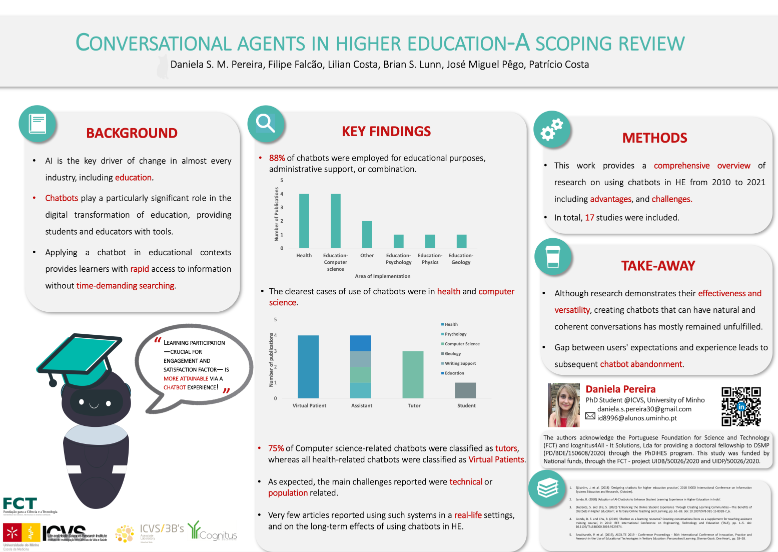
\includegraphics{Content/DEA2.png}

\newpage

\hypertarget{what-the-research-says-about-online-assessment-in-education}{%
\subsection{What the research says about online assessment in education}\label{what-the-research-says-about-online-assessment-in-education}}

\textbf{Authors:} Judicaël Alladatin, Insaf Al-Chikh, \& Eric Assogba

\textbf{Institution:} Université Mohammed VI Polytechnique

\textbf{Recommended Citation:}

\begin{quote}
Alladatin, J., Al-Chikh, I., \& Assogba, A. (2022, January 27). \emph{What the research says about online assessment in education} {[}Poster presentation{]}. Advancing Assessment and Evaluation Virtual Conference: Queen's University Assessment and Evaluation Group (AEG) and Educational Testing Services (ETS), Kingston, Ontario, Canada.
\end{quote}

\textbf{Abstract}

Assessment is considered a major concern in education due to the obvious function it plays with assessing individual student development as well as in measuring teaching effectiveness. Today, with the rapid growth of online and blended learning in education and its implementation in many education systems after COVID 19, online assessment has created new issues specific to the assessment of distance student performance. This article proposes a Strengths, Weaknesses, Opportunities, Threats (SWOT) analysis of the assessment practices and models from students, teachers, and institutions perceptions. The results indicate that the use of online learning assessments has many strengths, and opportunities, such as the capacity to perform tests on-demand and at any time, direct feedback to users, students' quick access to test results, and more precise evaluation of students' learning. Therefore, online assessment systems also have several weaknesses and threats, the technology is also not faultless and that internet connectivity issues may arise. There's also the price of the online evaluation software to be considered. In addition to teachers' and students' limited knowledge of technology.

\textbf{Poster}

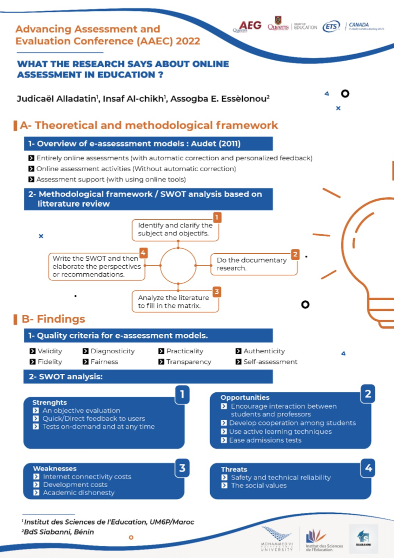
\includegraphics{Content/JA.png}

\newpage

\hypertarget{a-conversational-agent-to-measure-student-learning-conversation-based-assessment}{%
\subsection{A conversational agent to measure student learning: Conversation-based assessment}\label{a-conversational-agent-to-measure-student-learning-conversation-based-assessment}}

\textbf{Authors:} Seyma N. Yildirim-Erbasli \& Okan Bulut

\textbf{Institution:} University of Alberta

\textbf{Recommended Citation:}

\begin{quote}
Yildirim-Erbasli, S. N., \& Bulut, O. (2022, January 27). \emph{A conversational agent to measure student learning: Conversation-based assessment} {[}Poster presentation{]}. Advancing Assessment and Evaluation Virtual Conference: Queen's University Assessment and Evaluation Group (AEG) and Educational Testing Services (ETS), Kingston, Ontario, Canada.
\end{quote}

\textbf{Abstract}

One of the main goals of educational assessments is to obtain valid scores that reflect students' true ability levels. A major threat against the validity of educational assessments is the presence of non-effortful responses from unmotivated students. Due to insufficient interaction between learners and the non-interactive assessment environment, some students may get disengaged and fail to show effortful response behavior during the test. Unlike non-interactive assessments, interactive assessments (e.g., assessments involving one-on-one tutoring) allow students to work on a particular task and then review their responses to gain a better understanding of what they know. Therefore, interactive assessments can keep the students engaged in the assessment process while enabling them to communicate their knowledge more effectively. However, implementing interactive assessments in practice can be very challenging. Although such assessments are easy to use with a small number of students, they become more expensive and harder to implement with a large group of students. A promising solution to this problem is to create a conversation-based assessment (CBA) harnessing artificial intelligence (AI). The purposes of this study are twofold. First, we will create and implement an AI-based CBA that measures student learning and provides feedback interactively. Second, after students experience the CBA, we will examine students' attitudes towards CBA using an online survey. The CBA will be designed for an undergraduate course using Rasa----an AI-based system and deployed to a user-friendly environment (e.g., Google Chat). The CBA will ask questions, provide feedback on the quality of student responses, and hold social interactions through the natural flow of conversation. The findings of this study will help us understand the potential of CBAs in advancing conventional assessments (e.g., computer-based assessments) and increasing student motivation through interactivity that is missing in conventional assessments.

\textbf{Poster}

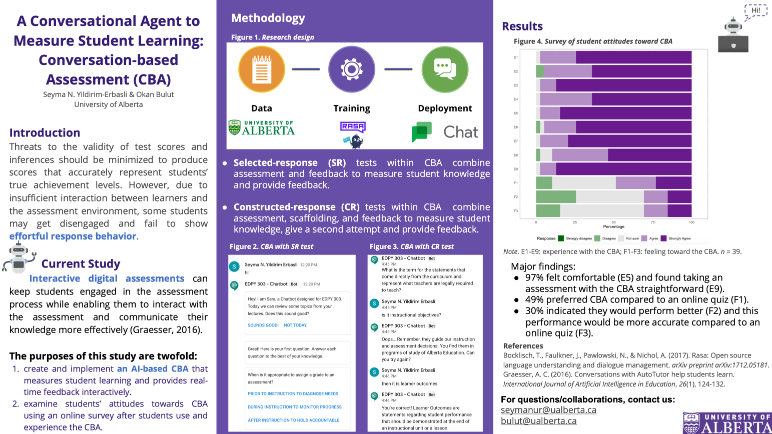
\includegraphics{Content/SO2.png}

\newpage

\hypertarget{impact-of-toefl-primary-tests-remote-proctored-tests-on-young-test-takers}{%
\subsection{Impact of TOEFL Primary Tests (Remote-Proctored Tests) on Young Test-Takers}\label{impact-of-toefl-primary-tests-remote-proctored-tests-on-young-test-takers}}

\textbf{Authors:} Jia Guo

\textbf{Institution:} Queen's University

\textbf{Recommended Citation:}

\begin{quote}
Guo, J. (2022, January 27). \emph{Impact of TOEFL Primary Tests (Remote-Proctored Tests) on Young Test-Takers} {[}Poster presentation{]}. Advancing Assessment and Evaluation Virtual Conference: Queen's University Assessment and Evaluation Group (AEG) and Educational Testing Services (ETS), Kingston, Ontario, Canada.
\end{quote}

\textbf{Abstract}

This study investigates the influence of online remote proctored young learners' test from test-takers and parents' perspective. This novel test delivery mode offers solution to the current situation of unexpected global COVID-19 pandemic where conventional on-site proctored tests are suspended amid the closure of test centers responding to the social distance requirement. In the long run, it also offers an alternative option to replace the conventional logistically complex and administratively challenging test delivery mode. In the context of young learners' English tests, ETS started offering remote-proctored delivered TOEFL Primary tests as an option for test-takers(ETS, 2021). There have been 825 young learners taking part in the trial version of the exam by the end of January 2021 in China(Chinanews, 2021). However, there is an absence of published research examining the influence of such a novel test delivery mode, and this study intends to bridge the gap. To achieve the research goal, Chapelle(2008)`s interpretive framework will be adopted to collect evidence. The multifaceted mixed-method approach will be used to investigate the influence of test delivery mode on young learners' test performance (explanation inference), test-takers' and their parents' perception and behavior (evaluation inference), and their interpretations and uses of test scores (utilization inference). The overall score and sub-scores of remote-proctored and on-site TOEFL Primary obtained from the official database will be compared and analyzed through descriptive statistics. Online questionnaires and interviews will be conducted among test-takers and parents participating in remote-proctored and on-site TOEFL Primary to obtain information about their perception, behavior, and interpretation and use of the test score. Quantitative and qualitative methods will be used to analyze the data. Demographic and geographic information will be taken into consideration in the analysis to help elicit the influence on test accessibility among different groups of population.

\textbf{Poster}

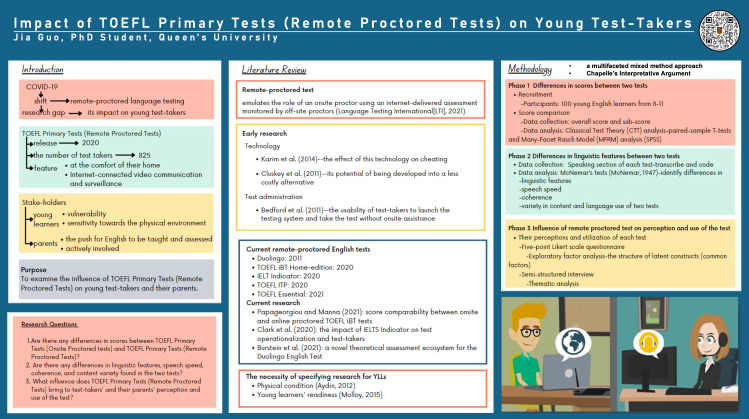
\includegraphics{Content/JG.png}

\newpage

\hypertarget{development-of-an-accessible-and-sensitive-measure-of-sustained-attention-the-3d-multiple-object-tracking-task}{%
\subsection{Development of an accessible and sensitive measure of sustained attention; The 3D Multiple Object Tracking task}\label{development-of-an-accessible-and-sensitive-measure-of-sustained-attention-the-3d-multiple-object-tracking-task}}

\textbf{Authors:} Taryn Perelmiter \& Dr.~Armando Bertone

\textbf{Institution:} McGill University

\textbf{Recommended Citation:}

\begin{quote}
Perelmiter, T., \& Bertone, A. (2022, January 27). \emph{Development of an accessible and sensitive measure of sustained attention; The 3D Multiple Object Tracking task} {[}Poster presentation{]}. Advancing Assessment and Evaluation Virtual Conference: Queen's University Assessment and Evaluation Group (AEG) and Educational Testing Services (ETS), Kingston, Ontario, Canada.
\end{quote}

\textbf{Abstract}

Current standardized measures of sustained attention are often limited due to their lack of generalizability, impurity of construct assessment, and inaccessibility for individuals with limited cognitive and/or language abilities. The 3D Multiple Object Tracking (3D-MOT) task is an intuitive, non-verbal paradigm previously demonstrated to isolate and assess sustained attention by manipulating the amount of time participants are asked to visually track target items from physically indistinguishable distractor items. We aimed to assess whether sustained attention measured using the 3D-MOT task would correlate to that of the Conners Continuous Performance Task (CPT-3), a current and clinically validated test of attention. Typically developing participants (n = 48, aged 13 to 30 years old) were recruited and were tested on both tasks. Exclusion criteria included obtaining a CPT-3 d' T-score greater than or equal to 60, indicating problems with general attention. A correlation was conducted comparing the percent change in average top speed score (\% change MOT score) between the longest (15 seconds) and shortest (5 seconds) trials in the MOT and the CPT-3 Hit Reaction Time (HRT) Block Change T-score, a sustained attention metric of the CPT-3. Results indicated that a small yet significant positive correlation (r = .299, p = .019) between the \% change MOT score and the HRT Block Change T-score on the CPT-3. This result supports the potential use of the 3D-MOT task as non-verbal measure of sustained attention in typically-developing participants. Future directions include replicating this study with a larger sample size, comparisons by age group (e.g., children, adolescents, adults), and comparisons of clinical (i.e., attention difficulty) versus non-clinical participants. This study represents a preliminary step towards validating the 3D-MOT task as an accessible and sensitive approach for assessing sustained attention for typically and atypically-developing populations.

\textbf{Poster}

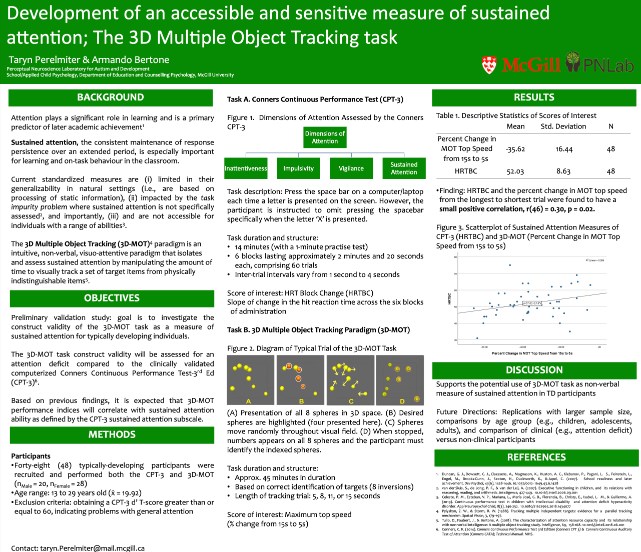
\includegraphics{Content/TA.png}

\newpage

\hypertarget{once-upon-an-algorithm-a-suggestive-approach-for-assessing-item-quality-usability-and-validity-of-automatic-item-generation}{%
\subsection{Once upon an Algorithm: A suggestive approach for assessing item quality, usability and validity of Automatic Item Generation}\label{once-upon-an-algorithm-a-suggestive-approach-for-assessing-item-quality-usability-and-validity-of-automatic-item-generation}}

\textbf{Authors:} Filipe Falcão, Daniela S. M. Pereira, Nuno Gonçalves, Patrício Costa, \& José M. Pêgo

\textbf{Institution:} School of Medicine, University of Minho

\textbf{Recommended Citation:}

\begin{quote}
Falcão, F., Pereira, D. S. M., Gonçalves, N., Costa, P., \& Pêgo, J. M. (2022, January 27). \emph{Once upon an Algorithm: A suggestive approach for assessing item quality, usability and validity of Automatic Item Generation} {[}Poster presentation{]}. Advancing Assessment and Evaluation Virtual Conference: Queen's University Assessment and Evaluation Group (AEG) and Educational Testing Services (ETS), Kingston, Ontario, Canada.
\end{quote}

\textbf{Abstract}

Background and objective: Automatic Item Generation (AIG) generates testing items through computer algorithms. The quality, usability and validity of AIG remains unexplored. This paper aims to assess AIG in medical assessment. Methods: Study I -- Participants with different levels of clinical knowledge and item writing experience developed items manually and using AIG. Items were compared regarding quality and usability; Study II -- Items generated by AIG were inserted in a summative exam in the area of surgery. Psychometric analysis were employed to inspect AIG's validity and item quality. Results: Study I -- Items generated by AIG presented quality. Time spent developing cognitive models and number of items generated did not vary between participants. Study II -- Items generated by AIG presented quality, were adequate for testing student's knowledge and presented evidence of validity. Conclusions: AIG is a valid method to produce numerous quality items in an easy and cost-effective process.

\textbf{Poster}

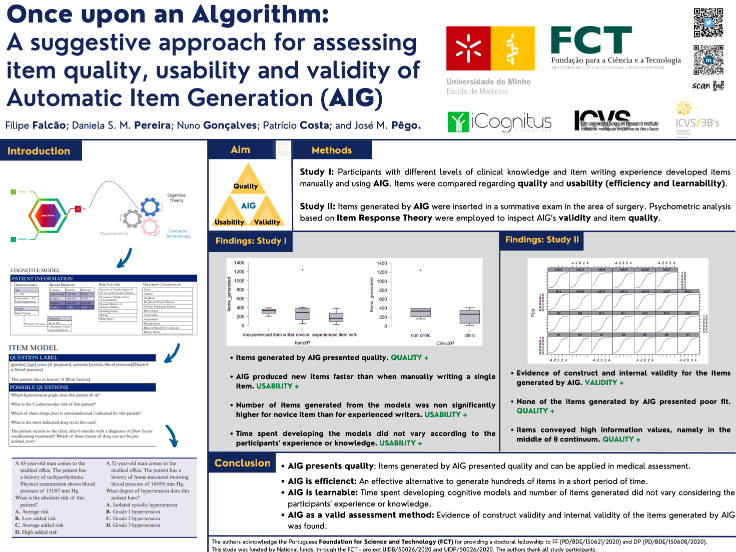
\includegraphics{Content/FF.png}

\newpage

\hypertarget{engineering-a-lasting-future-investigating-influences-on-the-self-efficacy-of-female-engineering-students}{%
\subsection{Engineering a Lasting Future: Investigating Influences on the Self-Efficacy of Female Engineering Students}\label{engineering-a-lasting-future-investigating-influences-on-the-self-efficacy-of-female-engineering-students}}

\textbf{Authors:} Nerissa Mulligan

\textbf{Institution:} Queen's University

\textbf{Recommended Citation:}

\begin{quote}
Mulligan, N. (2022, January 27). \emph{Engineering a Lasting Future: Investigating Influences on the Self-Efficacy of Female Engineering Students} {[}Poster presentation{]}. Advancing Assessment and Evaluation Virtual Conference: Queen's University Assessment and Evaluation Group (AEG) and Educational Testing Services (ETS), Kingston, Ontario, Canada.
\end{quote}

\textbf{Abstract}

Females and males have equal capabilities in math and science and are able to master mathematical and scientific concepts equally well, however, females continue to be underrepresented in Science, Technology, Engineering and Mathematics (STEM) education and professions. Numerous studies have shown that many female students leave engineering because of low self-efficacy and confidence, and many who persist have lower self-efficacy and confidence than their male counterparts. Self-efficacy is defined as an individual's belief in their own ability to achieve an outcome and is strongly influenced by academic accomplishments. Exploring the potential relationship between engineering programs and the self-efficacy of engineering students is critical to understanding student satisfaction, achievement, and retention in engineering programs. This study aims to fill the gap in knowledge regarding the differences in the sources of self-efficacy of male and female engineering students and the effects of the engineering curriculum on students' self-efficacy in the Canadian context. The research will focus on 1) measuring and identifying the sources of self-efficacy of male and female first-year engineering students; 2) investigating whether the sources of self-efficacy are different for male and female first-year engineering students and whether those sources change over time; and 3) measuring the effects of the first-year engineering curriculum on students' self-efficacy. Data will be gathered using an instrument developed for the study, based on several existing self-efficacy instruments, which will involve first-year engineering students at a mid-sized Canadian university completing a survey at the beginning and end of their first academic year. The results of this study will help guide university engineering programs toward closing the gender gap in STEM.

\textbf{Poster}

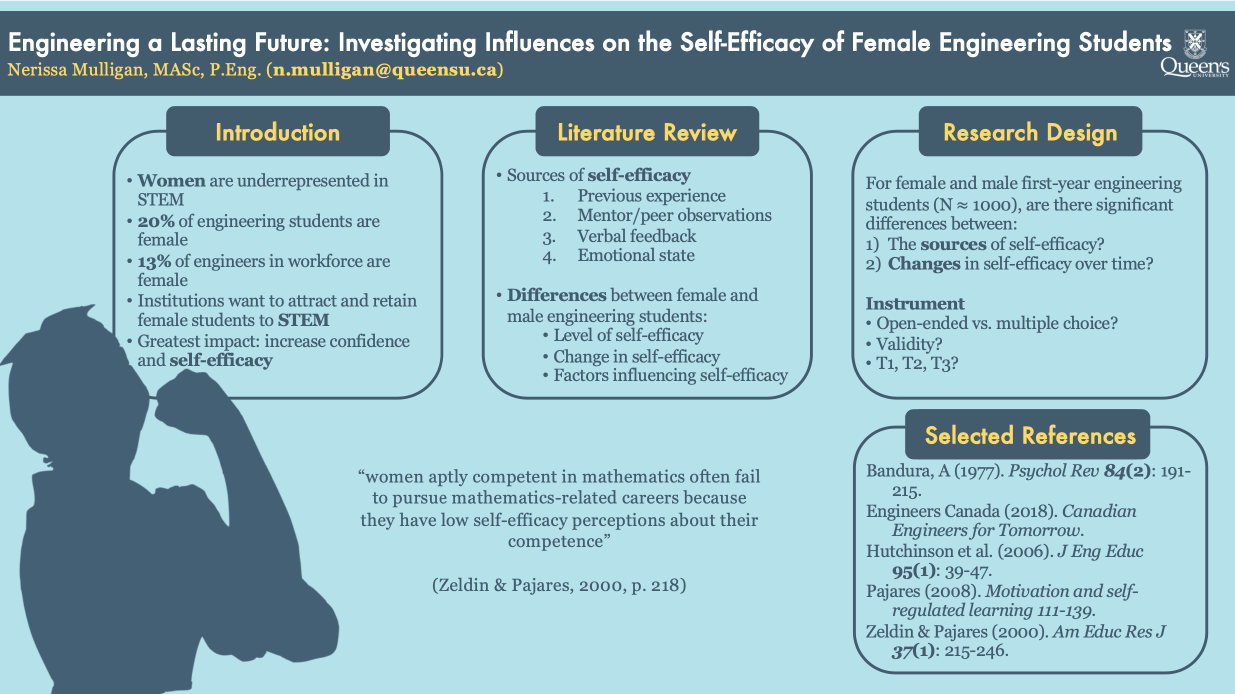
\includegraphics{Content/NM.png}

\newpage

\hypertarget{customizing-item-selection-with-engagement-in-computerized-adaptive-tests}{%
\subsection{Customizing Item Selection with Engagement in Computerized-Adaptive Tests}\label{customizing-item-selection-with-engagement-in-computerized-adaptive-tests}}

\textbf{Authors:} Guher Gorgun \& Okan Bulut

\textbf{Institution:} University of Alberta

\textbf{Recommended Citation:}

\begin{quote}
Gorgun, G., \& Bulut, O. (2022, January 27). \emph{Customizing Item Selection with Engagement in Computerized-Adaptive Tests} {[}Poster presentation{]}. Advancing Assessment and Evaluation Virtual Conference: Queen's University Assessment and Evaluation Group (AEG) and Educational Testing Services (ETS), Kingston, Ontario, Canada.
\end{quote}

\textbf{Abstract}

Purpose and Introduction: Test-taking disengagement is a significant validity threat for both computer-based and computerized adaptive tests (CATs), especially for those characterized as ``low-stakes''. It introduces construct-irrelevant variance (Finn, 2015; Haladyna \& Downing, 2004; Kong et al., 2007) and typically leads to the underestimation of examinees' true ability. In CATs, disengaged responses also jeopardize item selection as the selection of optimal items highly depends on the quality of responses. To minimize the negative influence of test-taking disengagement, the item selection algorithm in CATs can be modified to select the items that are not only suitable for the examinee's ability level but also engaging. Proposed Method: In this study, we propose to modify the maximum Fisher information (MFI) method to tailor the CAT item selection algorithm based on both each examinee's ability and engagement levels. With the proposed method, two sets of item information functions (IIFs) are estimated: one based on the examinee's interim ability, and another based on the examinee's test-taking engagement. Then, the product of these IIFs can be used to select the most optimal item. Results: We conducted a post-hoc simulation study using real data from 21,811 test-takers. We estimated two sets of item parameters based on dichotomous item responses (used for estimating ability) and dichotomized response times such that 1=optimal time use, 0=rapid guessing/slow responding (used for estimating engagement) and incorporated them into item selection in the CAT simulation. We found that the modified MFI method outperformed the conventional MFI method based on the correlations between true and estimated ability values, bias, and mean conditional standard error of measurement. The positive impact of incorporating test-taking engagement into item selection was the most evident for shorter tests (e.g., 20 items). Discussion: Our proposed method offers a proactive remedy to minimize disengagement in an operational low-stakes CAT setting.

\textbf{Poster}

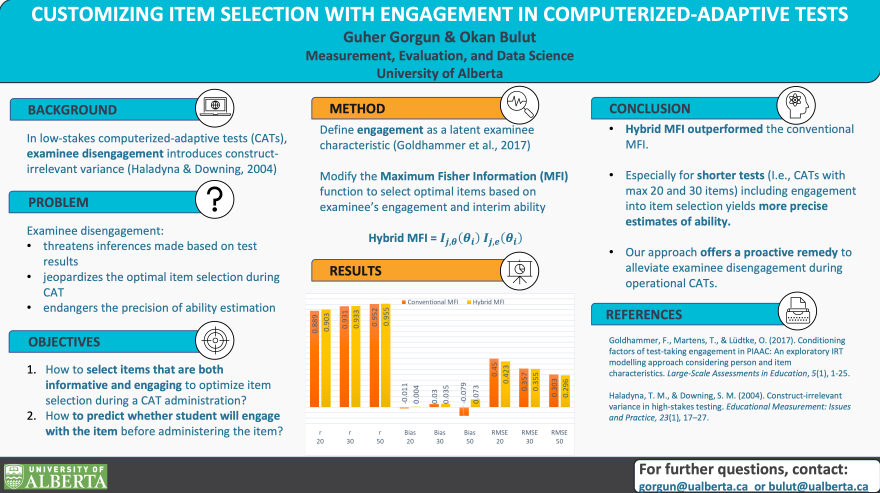
\includegraphics{Content/GO.png}

\newpage

\hypertarget{assessing-listening-difficulties-of-hard-of-hearing-students-in-general-education}{%
\subsection{Assessing Listening Difficulties of Hard of Hearing Students in General Education}\label{assessing-listening-difficulties-of-hard-of-hearing-students-in-general-education}}

\textbf{Authors:} Uvini Colonne

\textbf{Institution:} Queen's University

\textbf{Recommended Citation:}

\begin{quote}
Colonne, U. (2022, January 27). \emph{Assessing Listening Difficulties of Hard of Hearing Students in General Education} {[}Poster presentation{]}. Advancing Assessment and Evaluation Virtual Conference: Queen's University Assessment and Evaluation Group (AEG) and Educational Testing Services (ETS), Kingston, Ontario, Canada.
\end{quote}

\textbf{Abstract}

Classroom Introduction: With the widespread practice of early identification of hearing loss, advancement in hearing technology, and improvement of legislation have permitted hard of hearing students (HHSs) to experience education in each of the ten provinces and three territories in Canada. However, it is doubtful whether general education classrooms (GECs) are always adequately meet listening needs of this group of students with a compromised auditory system. Optimum classroom listening enables accessibility to language and communication, which are critical in students' academic success and positive social development. Aim: The purpose of this study is to determine listening difficulties faced by hard of hearing students in general education classrooms from both teachers' and students' perspective. Methods and analysis: A descriptive cross-sectional study will be conducted as an online survey through Qualtrics platform. Participants will be hard of hearing students attend in Eastern Ontario secondary GECs and their general education teachers. The teacher and student versions of a standardized questionnaire named Listening Inventory for Education-Revised (LIFE-R) LIFE-R will be used to evaluate teacher and student appraisals of the listening challenges in GECs. LIFE-R is composed of 15 questions which need to rate listening challenges in different situations following a scale between 1 to 5, representing no challenges to almost always challenged respectively. Quantitative data will be analysed using descriptive and inferential statistics. Ethics and dissemination: Ethical clearance for this study will be obtained from General Research Ethics Board at Queen's University, ON, and Eastern Ontario School Boards. Institutional clearance will be taken from the administration of individual public schools. Written informed consent will be obtained from all participants. Results will be disseminated, to local stakeholders and participants, via local and international conferences and publications in peer-reviewed journals.

\textbf{Poster}

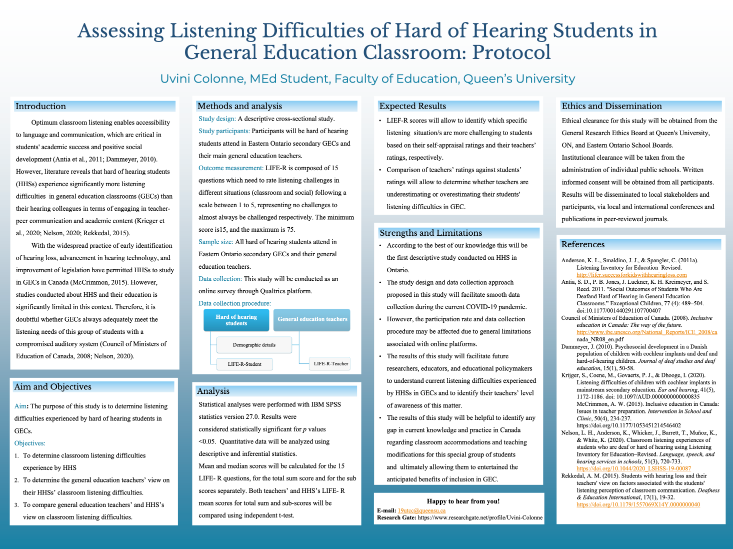
\includegraphics{Content/UC.png}

\newpage

\hypertarget{day-2-january-28-2022}{%
\section{Day 2: January 28, 2022}\label{day-2-january-28-2022}}

\hypertarget{automated-essay-scoring-in-multiple-languages-an-application-of-bert-to-persian-essay-scoring}{%
\subsection{Automated Essay Scoring in Multiple Languages: An Application of BERT to Persian Essay Scoring}\label{automated-essay-scoring-in-multiple-languages-an-application-of-bert-to-persian-essay-scoring}}

\textbf{Authors:} Tahereh Firoozi \& Mark Gierl

\textbf{Institution:} University of Alberta

\textbf{Recommended Citation:}

\begin{quote}
Firoozi, T., \& Gierl, M. (2022, January 28). \emph{Automated Essay Scoring in Multiple Languages: An Application of BERT to Persian Essay Scoring} {[}Poster presentation{]}. Advancing Assessment and Evaluation Virtual Conference: Queen's University Assessment and Evaluation Group (AEG) and Educational Testing Services (ETS), Kingston, Ontario, Canada.
\end{quote}

\textbf{Abstract}

One of the challenges in educational assessment is to reliably and efficiently evaluate students' written tasks. Human raters usually perform this task, but we need methods that scale more easily to large online courses or high stakes test-taking settings where there may be thousands or even millions of submissions that must be graded. Automatic essay scoring (AES) solves this problem by using computational models to automatically evaluate students' written tasks. Recently, with the advent of deep learning models, the accuracy of AES systems has significantly improved in a way that AES systems can now perform comparably to human raters in terms of their reliability and accuracy (Dong, Zhang, \& Yang, 2017). Studies have shown that deep learning models, including bidirectional transformers, can achieve state-of-the-art accuracy in AES (e.g., Lan et al., 2019). However, AES studies to-date have focused on exclusively on the English language with little focus on low resource languages such as Persian. The purpose of this study is to investigate the performance of BERT, a deep bidirectional transformer, for language understanding (Devlin, Chang, Lee, \& Toutanova, 2018) in the context of Persian essay scoring. BERT is a deep learning model in which every output element is connected to every input element, and the weightings between these elements are dynamically calculated based upon their connection. We used the BERT model to score 1,432 essays written by Persian speakers. The model was trained using 60\% of the essays (n=860) which contained labels assigned by the human raters based on the mastery level of each essay (i.e., elementary, intermediate, and advanced). Then, the accuracy of the trained model was tested on the remaining 40\% of the essays (n=572) which were unseen by the model. The model was very reliable (Cohen Kappa= 0.86) in predicting the essay scores producing a classification outcome that can be described as ``almost perfect agreement'' (Landis \& Koch, 1977). Results of this study bring evidence to the efficacy and dependability for using AES models to score written tasks in multiple languages.

\textbf{Poster}

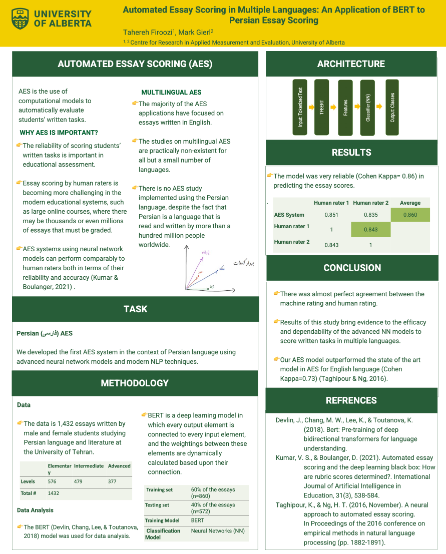
\includegraphics{Content/TM.png}

\newpage

\hypertarget{feedback-literacy-framework-in-the-e-assessment-context}{%
\subsection{Feedback Literacy Framework in the E-Assessment Context}\label{feedback-literacy-framework-in-the-e-assessment-context}}

\textbf{Authors:} Tarid Wongvorachan, Ka-Wing Lai, Okan Bukut, \& Yi-Shan Tsai

\textbf{Institution:} University of Alberta

\textbf{Recommended Citation:}

\begin{quote}
Wongvorachan, T., Lai, K., Bukut, O., \& Tsai, Y. (2022, January 28). \emph{Feedback Literacy Framework in the E-Assessment Context} {[}Poster presentation{]}. Advancing Assessment and Evaluation Virtual Conference: Queen's University Assessment and Evaluation Group (AEG) and Educational Testing Services (ETS), Kingston, Ontario, Canada.
\end{quote}

\textbf{Abstract}

For students, feedback received from their instructors can make a big difference in their learning by translating their assessment performance into future learning opportunities (Watling \& Ginsburg, 2019). To date, researchers have proposed various feedback literacy frameworks, which concern one's ability to interpret and use feedback for their learning, to promote students' feedback engagement by repositioning them as active participants in the learning process (Carless \& Boud, 2018). However, the current feedback literacy frameworks have not been adapted to digital or e-assessment settings despite the increasing use of e-assessments (e.g., computer-based tests, intelligent tutoring system) in practice. To address this gap, this conceptual paper introduces a feedback literacy model in the context of e-assessments to present an intersection between e-assessment features and the ecological model of feedback literacy for more effective feedback practices in digital learning environments. The general feedback literacy models posit that students' action on feedback can be influenced by the three dimensions of engagement (e.g., feedback appreciation aka cognitive engagement), contextual (e.g., curriculum), and individual (e.g., students' expertise on subject matter) (Chong, 2021). When applying this framework to e-assessments, personalized feedback and students' digital literacy can be attributed to the engagement dimension, while the use of computer-mediated communication (e.g., forum) and digital score reporting software can be attributed to the contextual dimension, and students' acceptance to e-assessments, including their perceived usefulness and credibility of the platform, could be attributed to the individual dimension of the model (Adenuga et al., 2019; Bulut et al., 2019, 2020; Liu et al., 2015). Aside from advocating for effective feedback practices, this paper will also demonstrate how to support the validity of score interpretations from e-assessments (AERA et al., 2014).

\textbf{Poster}

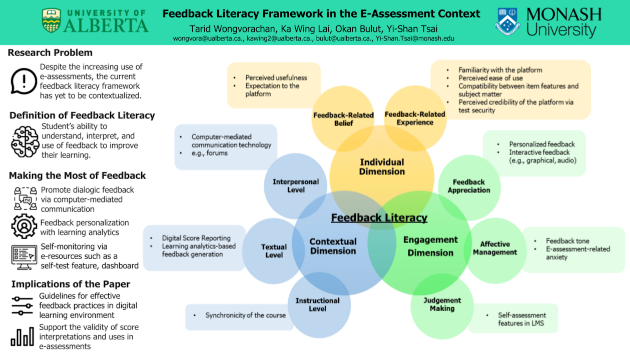
\includegraphics{Content/TW.png}

\newpage

\hypertarget{canoes-not-canals-assessing-emergent-learning-in-contemporary-classrooms}{%
\subsection{Canoes, not canals: Assessing emergent learning in contemporary classrooms}\label{canoes-not-canals-assessing-emergent-learning-in-contemporary-classrooms}}

\textbf{Authors:} Michael Holden

\textbf{Institution:} Queen's University

\textbf{Recommended Citation:}

\begin{quote}
Holden, M. (2022, January 28). \emph{Canoes, not canals: Assessing emergent learning in contemporary classrooms} {[}Poster presentation{]}. Advancing Assessment and Evaluation Virtual Conference: Queen's University Assessment and Evaluation Group (AEG) and Educational Testing Services (ETS), Kingston, Ontario, Canada.
\end{quote}

\textbf{Abstract}

Current research in classroom assessment is troubled by inconsistencies between a prevailing formative assessment framework and the kinds of learning that framework advances. On the one hand, scholars across the field emphasize formative assessment as an adaptive process, promoting inference and iteration as central concepts (Andrade, 2013; Earl, 2007; Kane, 2006). Since we cannot peek inside students' heads to measure whether they have learned something, or how well they have learned it, classroom assessment relies upon a teacher's ability to make adaptive inferences about what students are learning and how that learning might proceed (Bennett, 2011; Earl, 2007; Popham, 2009). At the same time, this adaptability is directly contradicted by widespread descriptions of learning as a fixed, predictable outcome (Stobart, 2008). Learning outcomes and progressions -- two hallmarks of contemporary formative assessment -- are often presented as ``blueprints for instruction'' that move learning from the teacher and curriculum to individual students in predictable patterns (Brookhart, 2003; Newton, 2017; Stobart, 2008). The purpose of this paper is to examine these contradictions and to call attention to emergent learning (novel and unpredictable learning that unfolds alongside instruction and assessment; Bolden \& DeLuca, 2016) as a central feature of classroom assessment. To do so, I employ a critical analysis of contemporary formative assessment research. In particular, I argue that without a framework that accounts for formative assessment's iterative and inferential core, teachers and researchers will struggle to achieve the kinds of classroom assessment we claim to hold dear. Emergent learning offers just such a framework, positioning assessment as ``a horizon rather than a fixed spot'' (Stobart, 2008, p.~156) such that teaching and learning are being formed. Such conceptions more closely reflect the spirit of formative assessment (Crossouard, 2011; Swaffield, 2011) and articulated goals of engaging students as meaningful actors in the classroom (Friesen, 2009).

\textbf{Poster}

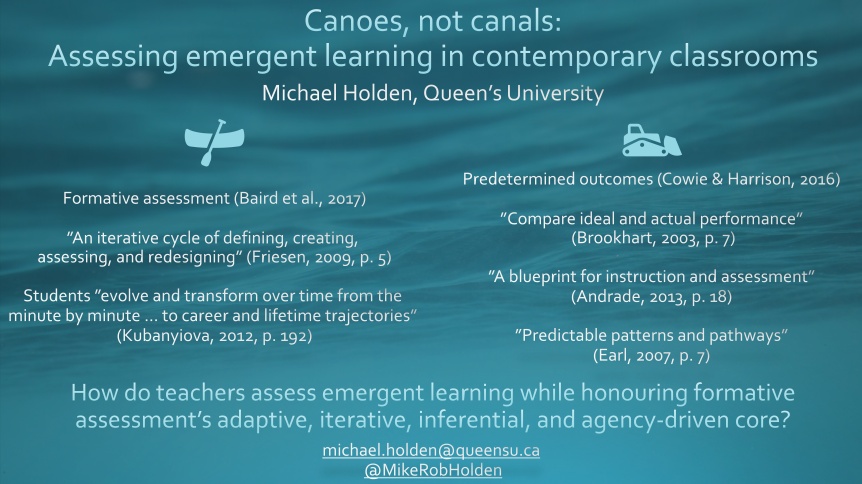
\includegraphics{Content/MH.png}

\newpage

\hypertarget{binary-and-nonbinary-gender-groups-impression-of-and-preference-for-computer-science-and-health-fields-as-college-majors-a-structural-equation-modeling}{%
\subsection{Binary and Nonbinary Gender Groups' Impression of and Preference for Computer Science and Health Fields as College Majors: A Structural Equation Modeling}\label{binary-and-nonbinary-gender-groups-impression-of-and-preference-for-computer-science-and-health-fields-as-college-majors-a-structural-equation-modeling}}

\textbf{Authors:} Yue Mao, Sirui Wu, Jake E. Stone, \& Amery D. Wu

\textbf{Institution:} University Of British Columbia

\textbf{Recommended Citation:}

\begin{quote}
Mao, Y., Wu, S., Stone, J. E., \& Wu, A. D. (2022, January 28). \emph{Binary and Nonbinary Gender Groups' Impression of and Preference for Computer Science and Health Fields as College Majors: A Structural Equation Modeling} {[}Poster presentation{]}. Advancing Assessment and Evaluation Virtual Conference: Queen's University Assessment and Evaluation Group (AEG) and Educational Testing Services (ETS), Kingston, Ontario, Canada.
\end{quote}

\textbf{Abstract}

The purpose of this study was to compare male, female, and non-binary gender groups' impression of and preference for computer science (CS) and health fields (HL), two fields that are high in demand and short in labor supply. Gender gaps persist in CS and HL college majors. It is essential to investigate these gaps at an early stage. Thus, the current study investigated the ``prospective'' students' impression of and preference for CS and HL based on 13,569 participants' responses to the College Major Preference Assessment. Compared to males, a smaller proportion of females chose CS (2\% vs 6\%), and more females chose HL as their favorite (23\% vs 14\%). Significant gender differences were found in both latent impression and preference using structural equation modelling. Compared to male youth, female youth held a statistically significant lower impression of and preference for CS, and the opposite was found for HL. As for the binary gender group, their choice was more akin to that of the male group for both CS and HL; The only difference is that their impression of HL was noticeably more positive. Although our study was purely about individuals' impression and preference, the findings on gender difference were consistent with the reports of ``actual major.'' This consistency supports the belief that gender difference in the actual major was reflective of the difference in impression and preference (e.g., Gemici \& Wiswall, 2014; Turner \& Bowen, 1999). Thus, understanding how early impression and preference are formed is worth a future study and is crucial to promoting gender equity. To our best knowledge, this study is the first to reveal the nonbinary group's inclination towards college majors. Future investigation can investigate why their impression and preference are more akin to males.

\textbf{Poster}

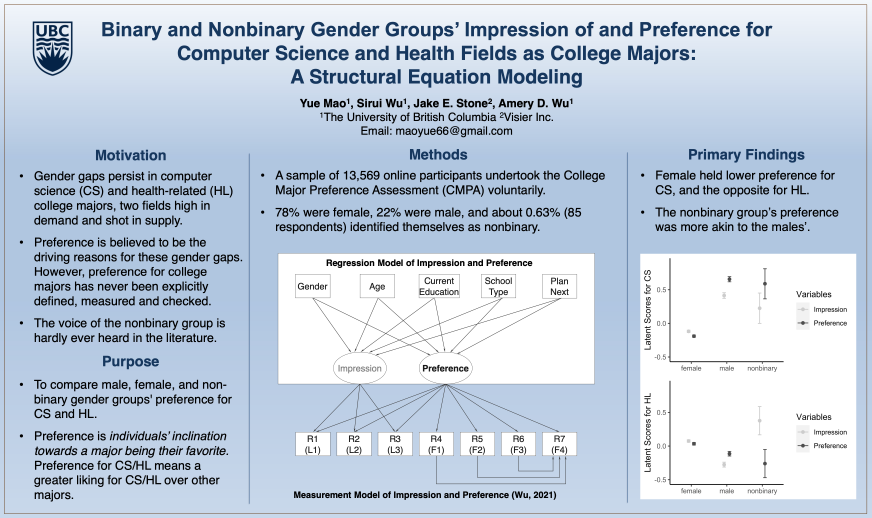
\includegraphics{Content/YU.png}

\newpage

\hypertarget{how-do-you-feel-about-hearing-practicing-teachers-thoughts-examining-pre-service-teachers-perceptions-of-assessment-with-a-control-value-theory-lens}{%
\subsection{How do you feel about hearing practicing teachers' thoughts?: Examining pre-service teachers' perceptions of assessment with a control-value theory lens}\label{how-do-you-feel-about-hearing-practicing-teachers-thoughts-examining-pre-service-teachers-perceptions-of-assessment-with-a-control-value-theory-lens}}

\textbf{Authors:} Kendra Wells, Bryce S. Dueck, \& Lia M. Daniels

\textbf{Institution:} University of Alberta

\textbf{Recommended Citation:}

\begin{quote}
Wells, K., Dueck, B. S., \& Daniels, L. M. (2022, January 28). \emph{How do you feel about hearing practicing teachers' thoughts?: Examining pre-service teachers' perceptions of assessment with a control-value theory lens} {[}Poster presentation{]}. Advancing Assessment and Evaluation Virtual Conference: Queen's University Assessment and Evaluation Group (AEG) and Educational Testing Services (ETS), Kingston, Ontario, Canada.
\end{quote}

\textbf{Abstract}

Purpose: The purpose of this poster is to describe pre-service teachers' emotions in response to learning about classroom assessment through ``Teacher Talks'' -- video interviews with practicing teachers designed to link theory to practice. Context: Assessment is an emotional experience for teachers and students (Brackett et. al, 2013; Kiuru et. al, 2020). University Education programs offer opportunities for pre-service teachers to learn about assessment theory and practice. During this time, students begin to experience assessment from an in-service teacher perspective which may introduce emotions. Control-value theory proposes that certain emotions are elicited by varying levels of value and control appraisals about a learning situation. Pekrun (2006) theorizes that frustration and enjoyment are oppositely valenced activity emotions elicited from perceptions of low control or from high control and value respectively. Methodology: As part of the assessment course, students (n=184) watched ``Teacher Talks'' and rated the extent to which the videos supported their sense of control and value. We measured several emotional responses including frustration and enjoyment. Results: We used two regression analyses to test the relationship between control and value appraisals and emotions. A value appraisal was more significantly tied to frustration and enjoyment than a control appraisal. Control (b=-.029, p=0.664) and value (b=-.573, p\textless.001) were negative predictors of frustration and explained 33.7\% of the variance. Control (b=.134, p=.019) and value (b=.673, p\textless.001) were positive predictors of enjoyment and explained 54.6\% of the variance. Discussion: These results indicate that pre-service teachers who valued and perceived greater control related to assessment through the Teacher Talks felt more enjoyment. In contrast, when the students did not value the Teacher Talks, they became frustrated. As instructors design opportunities to learn about classroom assessment it is important to maximize perceptions of control and value.

\textbf{Poster}

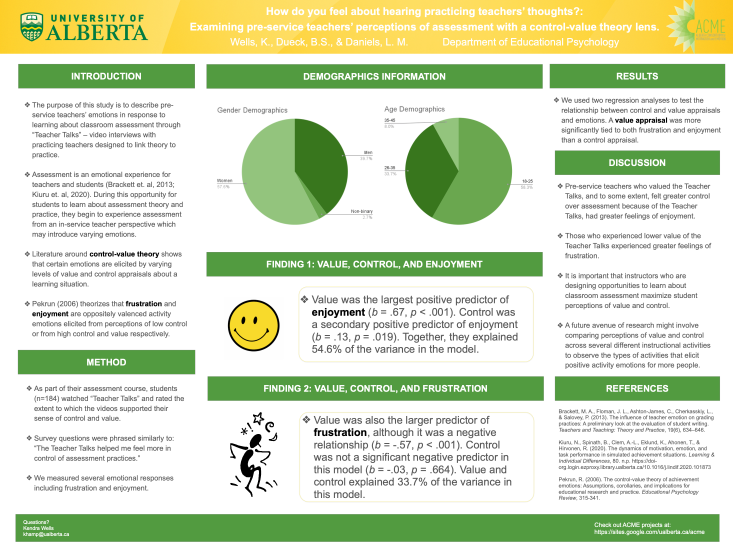
\includegraphics{Content/KW.png}

\newpage

\hypertarget{assessing-identity-awareness-and-cultural-responsiveness-for-pre-service-teachers-in-quebec-development-of-a-province-wide-tool}{%
\subsection{Assessing Identity Awareness and Cultural Responsiveness for Pre-service Teachers in Quebec: Development of a Province Wide Tool}\label{assessing-identity-awareness-and-cultural-responsiveness-for-pre-service-teachers-in-quebec-development-of-a-province-wide-tool}}

\textbf{Authors:} Welly Minyangadou Ngokobi

\textbf{Institution:} McGill University

\textbf{Recommended Citation:}

\begin{quote}
Minyangadou Ngokobi, W. (2022, January 28). \emph{Assessing Identity Awareness and Cultural Responsiveness for Pre-service Teachers in Quebec: Development of a Province Wide Tool} {[}Poster presentation{]}. Advancing Assessment and Evaluation Virtual Conference: Queen's University Assessment and Evaluation Group (AEG) and Educational Testing Services (ETS), Kingston, Ontario, Canada.
\end{quote}

\textbf{Abstract}

Assessment and Evaluation are means of measuring learners' understanding of the knowledge transferred to them. When it comes to teacher training, pre-service teachers are assessed and evaluated throughout their certifications in various ways depending on the institution through which they undergo said training. As learners themselves and regardless of the training program they subscribe to, pre-service teachers must all successfully demonstrate mastery of all professional competencies as required by the Ministry of Education. ``Competency 1: To act as a cultural facilitator when carrying out duties'' and ``Competency 8: Support student's love for learning'' being two of them. Pedagogy that engages in deep consideration of the intersectionalities that come with student diversity is taught in many teacher training programs. However, how thorough and consistent are its assessments and evaluations across universities? In other words, how do academic institutions ensure that their pre-service teachers have the required knowledge and tools to successfully lead a multicultural classroom and navigate complicated situations that stem from the students' racial, social, and gendered differences? I contribute to the ongoing conversations around the importance of student identity awareness and cultural responsiveness in learning environments through developing a preliminary framework and tool for assessing these professional competencies. The research is fueled by theoretical considerations rooted in Dewey's concept of Reformed Education. I review current assessments on teacher's cultural responsiveness and identity awareness, and analyze them through a critical race theory lens to create a novel assessment contextualized to the QEP. I will present a preliminary comprehensive assessment and evaluation grid that measures, in a fair and equitable manner across university programs, pre-service teachers' student identity awareness and cultural responsiveness. This assessment and evaluation grid must be seamlessly implementable and adaptable to all university teacher training programs and must enable pre-service teachers to practice, reflect on, and most importantly, receive timely, specific, and pertinent feedback on their demonstration of knowledge and mastery of Competency 1 and 8 of the QEP in learning situations. Keywords: pedagogy, curriculum, assessment and evaluation, teacher training, identity awareness, cultural responsiveness.

\textbf{Poster}

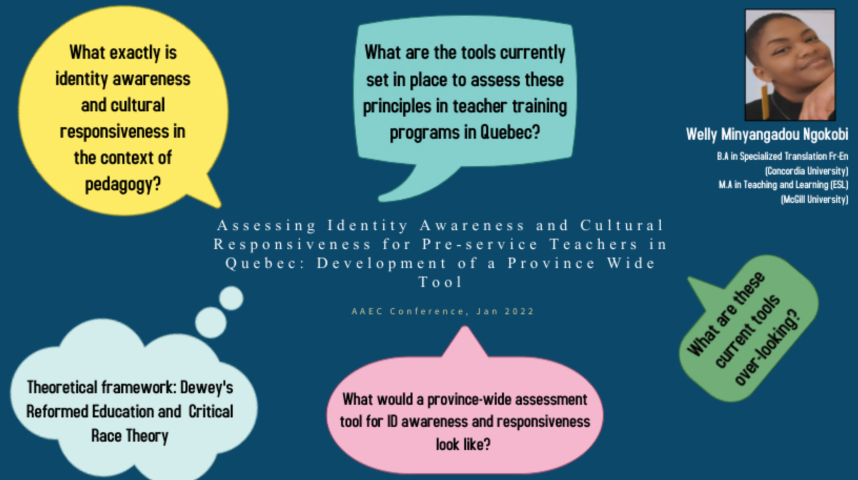
\includegraphics{Content/WM.png}

\newpage

\hypertarget{teaching-asynchronously-during-the-covid-19-pandemic-experiences-and-reflections-of-four-teaching-assistants}{%
\subsection{Teaching Asynchronously during the COVID-19 Pandemic: Experiences and Reflections of four Teaching Assistants}\label{teaching-asynchronously-during-the-covid-19-pandemic-experiences-and-reflections-of-four-teaching-assistants}}

\textbf{Authors:} Bryce Dueck \& Lia Daniels

\textbf{Institution:} University of Alberta

\textbf{Recommended Citation:}

\begin{quote}
Dueck, B., \& Daniels, L. (2022, January 28). \emph{Teaching Asynchronously during the COVID-19 Pandemic: Experiences and Reflections of four Teaching Assistants} {[}Poster presentation{]}. Advancing Assessment and Evaluation Virtual Conference: Queen's University Assessment and Evaluation Group (AEG) and Educational Testing Services (ETS), Kingston, Ontario, Canada.
\end{quote}

\textbf{Abstract}

The purpose of this poster is to reflect on the experiences of four Teaching Assistants (TAs) of the mandatory undergraduate classroom assessment course at the University of Alberta in Fall 2021. At the University of Alberta all undergraduate pre-service teachers take a required classroom assessment course (EDPY 303) during their ``Introductory Professional Term'' (IPT). The IPT is a condensed semester in which students take a full credit course in 9 weeks before their first practicum placement. EDPY 303 is a large course and is taught separately to pre-service teachers in the elementary and secondary programs. In Fall 2020, the course was taught online as required by the public health restrictions associated with the COVID-19 pandemic. The course was so well received by students that in Fall 2021 the instructor elected to offer the course in the same delivery format. The four TAs used a reflective case study approach (Becker \& Renger, 2016) to explore the unique experience of TAing EDPY 303 during the ongoing COVID-19 pandemic. Each TA identified their main opportunities and challenges and then discussed them as a team. The TAs identified the following opportunities including helping students to navigate online learning, finding novel ways to facilitate learning and learning how to support students with accommodations taking an online course. Challenges included connecting with students, managing student dissatisfaction and workload. Learning about classroom assessment is an important part of teacher education. In Alberta, an entire Teaching Quality Standard (TQS 3C; 2020) is dedicated to application of assessment and evaluation practices that support student learning, equity, and fairness. The role of TA in such learning experiences is important but also stressful, particularly during the COVID-19 pandemic as students have many questions about assessment as it pertains to not only their coursework, but also their future as teachers.

\textbf{Poster}

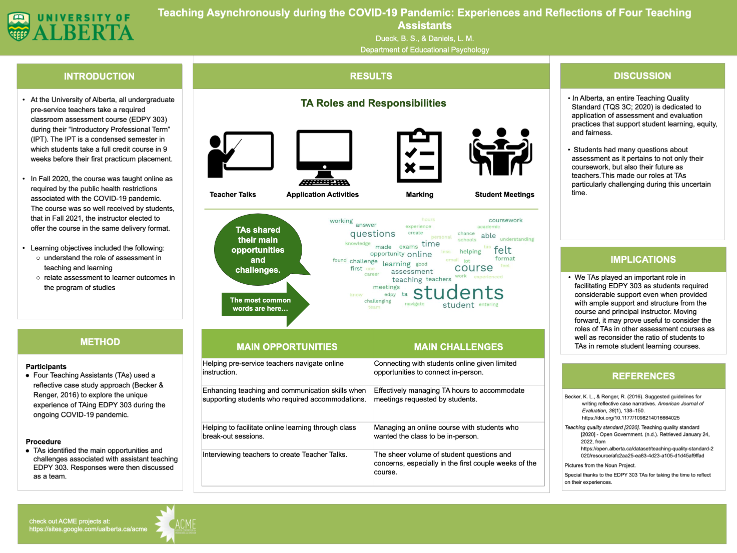
\includegraphics{Content/DD.png}

\newpage

\hypertarget{chinese-students-conceptions-of-feedback-and-their-relationships-with-self-regulated-learning-self-efficacy-and-english-language-achievement-in-the-college-english-class}{%
\subsection{Chinese Students' Conceptions of Feedback and their Relationships with Self-Regulated Learning, Self-Efficacy and English Language Achievement in the College English Class}\label{chinese-students-conceptions-of-feedback-and-their-relationships-with-self-regulated-learning-self-efficacy-and-english-language-achievement-in-the-college-english-class}}

\textbf{Authors:} Shasha Lu

\textbf{Institution:} Queen's University

\textbf{Recommended Citation:}

\begin{quote}
Lu, S. (2022, January 28). \emph{Chinese Students' Conceptions of Feedback and their Relationships with Self-Regulated Learning, Self-Efficacy and English Language Achievement in the College English Class} {[}Poster presentation{]}. Advancing Assessment and Evaluation Virtual Conference: Queen's University Assessment and Evaluation Group (AEG) and Educational Testing Services (ETS), Kingston, Ontario, Canada.
\end{quote}

\textbf{Abstract}

Under the influence of examination-driven culture and teacher-centered way of learning, Chinese students' self-regulated learning (SRL) capabilities, their self-efficacy as a motivational factor, and their actual English proficiency are underdeveloped. Given this situation, the Chinese Ministry of Education has promulgated the use of formative assessment in the College English curriculum at the tertiary level since 2004. Feedback, as an integrated part of formative assessment, is to facilitate learning and SRL, especially in higher education. However, whether feedback could facilitate students' SRL has not been fully investigated at the tertiary context in China. Therefore, this study aims to explore the relationships among students' conceptions of feedback, their SRL, self-efficacy, and English language achievement in the College English class in China. This study will use a quantitative method research design. A questionnaire will be used to collect data. Students' conceptions of feedback will be measured by Student Conceptions of Feedback Questionnaire. SRL strategies and self-efficacy can be measured by the Metacognitive Self-Regulation subscale and the Self-efficacy for Learning and Performance subscale of the Motivated Strategies for Learning Questionnaire (MSLQ). A 5-point Likert scale will be adopted. There are altogether 58 items. Their English test score as an indicator of English language achievement will also be collected. Participants will include approximately 500 students from a university in Northern China. Data will be analyzed using descriptive statistics, exploratory factor analyses, Pearson correlation analyses and multiple regression analyses. From the theoretical perspective, this study could address the research gap in the literature by examining the four constructs, i.e., student conceptions of feedback, SRL, self-efficacy and English language achievement in a different context in China. From the pedagogical angle, it is crucial to support teachers on their feedback practices to facilitate students' SRL, self-efficacy and learning.

\textbf{Poster}

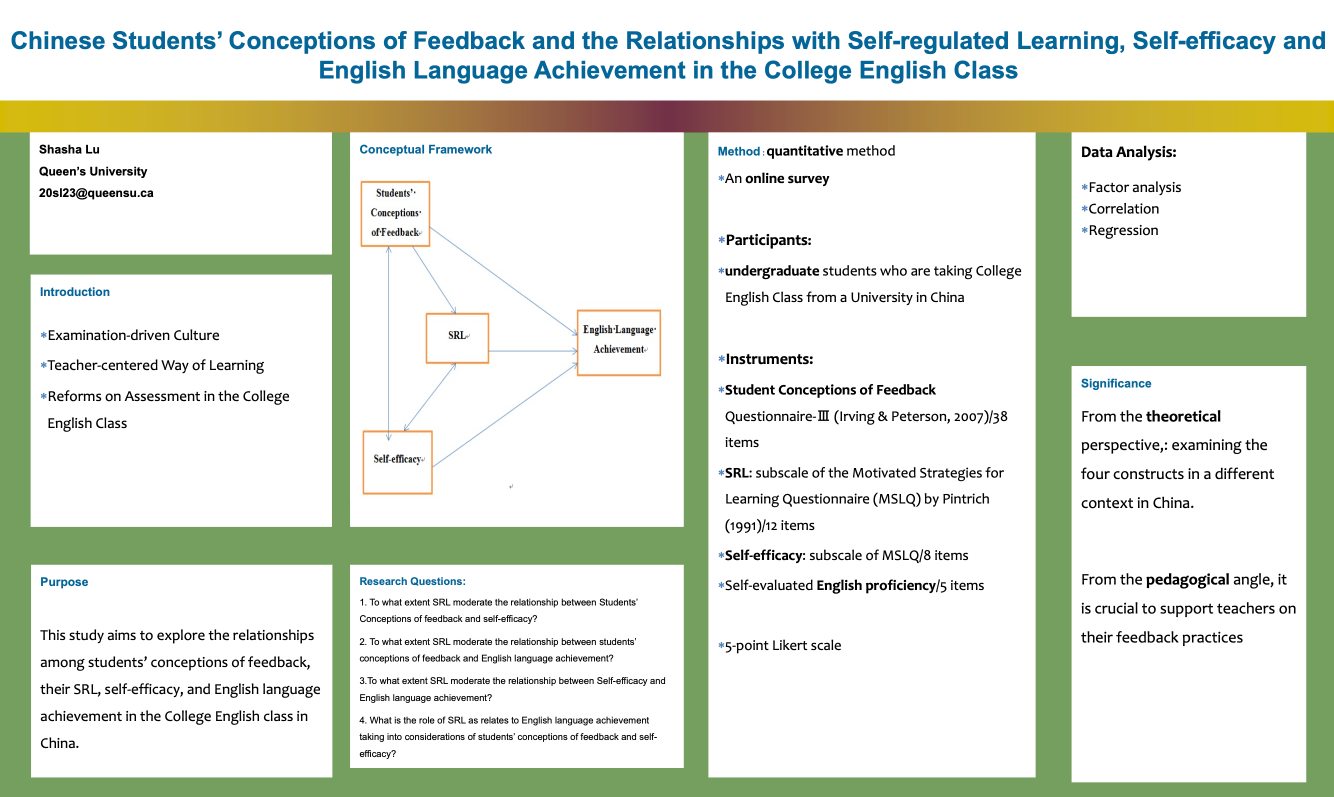
\includegraphics{Content/SL.png}

\newpage

\hypertarget{falling-between-the-cracks---compounding-identity-discrimination-within-healthcare}{%
\subsection{Falling between the cracks - Compounding identity discrimination within healthcare}\label{falling-between-the-cracks---compounding-identity-discrimination-within-healthcare}}

\textbf{Authors:} Jane Mao

\textbf{Institution:} Queen's University

\textbf{Recommended Citation:}

\begin{quote}
Mao, J. (2022, January 28). \emph{Falling between the cracks - Compounding identity discrimination within healthcare} {[}Poster presentation{]}. Advancing Assessment and Evaluation Virtual Conference: Queen's University Assessment and Evaluation Group (AEG) and Educational Testing Services (ETS), Kingston, Ontario, Canada.
\end{quote}

\textbf{Abstract}

Transgender and/or gender non-conforming (TGNC) individuals are one of the most underserviced populations in the Canadian healthcare system, as they face higher rates of unmet healthcare needs, lower quality of health services, and express greater mistrust of clinicians compared to their cisgender counterparts. A major barrier to patients accessing high-quality care is limited and inaccurate clinical education about the TGNC community; this means that a primary care physician's (PCP) lack of adequate training and knowledge can hinder a TGNC patient's access to treatment and long-term follow-up care. In parallel to TGNC experiences, racialized (i.e., non-white) patients also often face higher rates of unmet health needs that stem from a healthcare provider's cultural incompetency and racial bias, resulting in a variety of health disparities compared to their white counterparts. Some forms of discrimination against racialized patients are stereotyping and biases of racialized patients during clinical encounters. This proposed project seeks to examine gaps in Canadian PCP care for racialized TGNC individuals by analyzing the impacts of gender, gender identity, and race discrimination in PCP practices in order to improve the quality of life of gender-diverse people of colour. Using the findings of this study, medical educators and medical professional associations can begin closing this equity gap in healthcare access. A shift to inclusive healthcare is necessary for Canadian healthcare in order to align with the World Professional Association for Transgender Health's (2012) and National Collaborating Centre for Indigenous Health's (2020) standard of care. Furthermore, I will work to incorporate active learning measures to counter adverse experiences by applying my findings to medical education, via hosting training and information sessions on incorporating and expanding inclusive care with stakeholders such as Queen's Faculty of Medicine, and creating assessments to analyze the efficacy, knowledge retention, of our medical education programming.

\textbf{Poster}

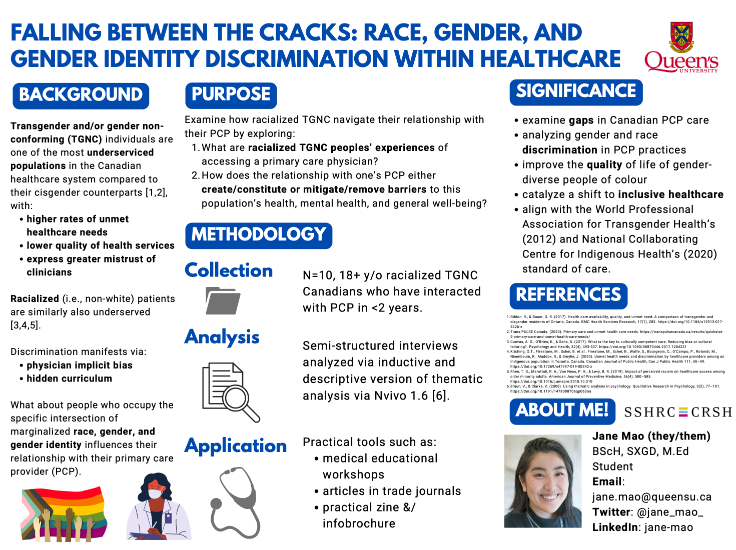
\includegraphics{Content/JM.png}

\newpage

\hypertarget{french-immersion-teachers-perspectives-of-translanguaging-as-a-theory-and-pedagogy}{%
\subsection{French Immersion Teachers' Perspectives of Translanguaging as a Theory and Pedagogy}\label{french-immersion-teachers-perspectives-of-translanguaging-as-a-theory-and-pedagogy}}

\textbf{Authors:} Francois-Daniel Levasseur-Portelance

\textbf{Institution:} Queen's University

\textbf{Recommended Citation:}

\begin{quote}
Levasseur-Portelance, F. D. (2022, January 28). \emph{French Immersion Teachers' Perspectives of Translanguaging as a Theory and Pedagogy} {[}Poster presentation{]}. Advancing Assessment and Evaluation Virtual Conference: Queen's University Assessment and Evaluation Group (AEG) and Educational Testing Services (ETS), Kingston, Ontario, Canada.
\end{quote}

\textbf{Abstract}

The emerging theory of Translanguaging challenges the notion that language systems are cognitively independent rather than interactive and social structures (Garcia \& Wei, 2014). The continuum of an individuals' language repertoire evolves by interacting with the knowledge of other languages and cultures in which the individual lives (Garcia, 2009). This practice may have positive implications for French Immersion (FI) programs in Ontario as an extension of the additive bilingual model currently in place. Good bi/multilingual education empowers those being educated, effectively placing the speaker at the heart of the interaction (Tupas \& Martin, 2017). Longitudinal studies have found that the strongest predictors of student success in their second language (L2) relates to the amount of formal instruction received in their first language (L1) (Ramirez et al., 1991; Thomas \& Collier, 2002). Furthermore, innovative pedagogies such as translanguaging may offer powerful spaces for educators to engage with their own multilingualism in a more complex manner (Weinmann, \& Charbonneau, 2020). However, little research has been conducted on understanding language teachers' perspectives and beliefs about bi/multilingualism, and their teaching practices (e.g.,Van Der Wildt et al., 2017).

\textbf{Poster}

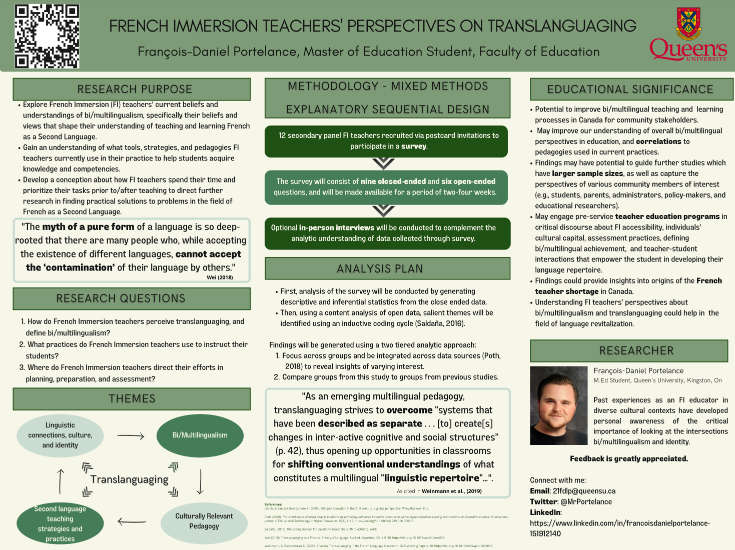
\includegraphics{Content/FDP.png}

\newpage

\hypertarget{empower-computational-thinking-skills-of-pre-service-teachers-at-university-level}{%
\subsection{Empower Computational Thinking skills of pre-service teachers at University Level}\label{empower-computational-thinking-skills-of-pre-service-teachers-at-university-level}}

\textbf{Authors:} Yimei Zhang

\textbf{Institution:} McGill University

\textbf{Recommended Citation:}

\begin{quote}
Zhang, Y. (2022, January 28). \emph{Empower Computational Thinking skills of pre-service teachers at University Level} {[}Poster presentation{]}. Advancing Assessment and Evaluation Virtual Conference: Queen's University Assessment and Evaluation Group (AEG) and Educational Testing Services (ETS), Kingston, Ontario, Canada.
\end{quote}

\textbf{Abstract}

Empower Computational Thinking skills of pre-service teachers at University Level Context \& Purpose Computational Thinking as a cognitive skill is applicable in problem solving process and can have a positive impact over time on inquiry skills in Mathematical / science classrooms to improve intellectual growth and analytical abilities for students (Weintrop, Beheshti, Horn, Orton, Jona, Trouille \& Wilensky, 2016). How to define and evaluate the development of CT skills while making it more accessible and inclusive by embedding it in existing curriculum deserves researching, especially on pre-service teachers (Brennan \& Resnick, 2012). Two purposes: 1) How the assessment we design for assessing CT skills can foster pre-service teachers' teaching / learning abilities in the classrooms 2) Evaluate the impact of projects that pre-service teachers are exposed to on their ability to transfer their computational thinking skills to pedagogical activities. Methodology \& Hypotheses: Participants in this mixed-method research design (Creswell, 1999) will be recruited from Department of Education at McGill. Quantitative and qualitative data will be collected over 2022 winter semester. Experimental research, (Ros \& Morrison, 2013) including Control and Experimental groups, will be tested by taking into account several potentially confounding variables (i.e., gender, major, year of study), while the primary variable is the project for designing CT pedagogical frameworks pre-service teachers will be assigned. Three--stage individual semi-structed interviews / questionnaires from the beginning, mid-term and ending will take place between researchers and participants for assessing their development of CT skills in their teaching practices/understanding. The assessment I apply will include ``Computational Theories, Practices, Perspectives''. Two hypotheses will be tested: 1. the assessment we design are conductive to pre-service teachers' CT skills in teaching and learning. 2. Promote pre-service teachers' ability to apply the evaluation abilities for demystifying / developing CT skills is critical in professional education.

\textbf{Poster}

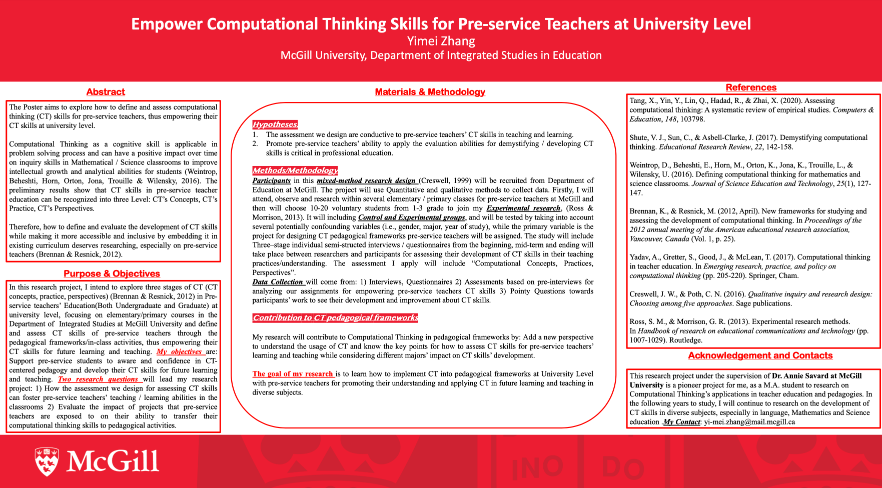
\includegraphics{Content/YZ.png}

\newpage

\hypertarget{conclusion}{%
\chapter*{Conclusion}\label{conclusion}}
\addcontentsline{toc}{chapter}{Conclusion}

The conference organizers thank all who participated in the inaugural Advancing Assessment and Evaluation Conference, with a special thank you to our poster presenters, panelists, and discussants. Presenting in a virtual format can be challenging, but all presentations were engaging, thought-provoking, and enabled rich discussion. We appreciate the attendees remaining engaged as well. As conference organizers, our hope is that the presentations and follow-up questions and rich discussion contributes to the assessment and evaluation community in Canada to propel our field and research. Taking what we learned from this conference, the Assessment and Evaluation Group (AEG) at Queen's University and ETS Canada very much look forward to planning our next event.

Sincerely,

AAEC Planning Committee


\includegraphics{Content/PC.png}

\newpage

  \bibliography{book.bib,packages.bib}

\end{document}
